\chapter{Measurement System Design}
\label{chap3}

\section{Introduction}

The goal of this project is to determine the pose estimation accuracy of a quadcopter flying in the outdoors. In this context, the pose is a six-dimensional position and orientation vector.

In order to determine a quadcopter's pose estimation accuracy, two sets of data are required: the first is the quadcopter's own pose estimate and the second its true pose, as measured by an accurate external measurement tool. There are accurate measurement tools available for the outdoor environment, which include laser and sonar systems. However, they are fairly expensive systems. It was therefore decided to investigate an alternative method of measuring a quadcopter's true pose in the outdoors.

A computer vision-based system was investigated and later implemented. Using a computer vision system (CVS) for measurement is an attractive option due to it being simple, cheap, compact and easy to operate. However, the measurement accuracy of these systems differ between platforms. Therefore, a method of reliably determining a CVS's pose measurement accuracy must also be developed before it can be used to make pose measurements of a quadcopter. 

This chapter sets out to provide detail on the design process of the CVS.\@ First, the design and layout of the CVS is discussed. Then, the method employed to determine the pose measurement accuracy is provided. Finally the results of the entire process, from testing to data processing, are discussed.

\section{Computer Vision System Layout}
\label{sec:chap3-cvs-layout}

The CVS has both hardware and software components, both of which are important to making accurate pose measurements. In this section, the layout and design of the CVS, including its hardware and software components, are discussed, providing a broad overview of the system's make-up and how it functions. 

\subsection{System Overview and Requirements}

The CVS is meant to measure the pose of a quadcopter in flight. It does this by using a calibrated camera to track a calibration board stuck to the object whose pose is to be measured (the quadcopter in this case). It then follows the next steps to determine the object's pose. These steps are explained in more detail in this section. 

\begin{enumerate}
  \item Detect and track the feature data of the calibration board, e.g.\ corners or dots on a flat board. 
  \item Extract two-dimensional coordinates of the features.
  \item Use a Principle n-Points solver with two-dimensional coordinates to determine the six-dimensional pose of the object relative to the camera. 
\end{enumerate}

The CVS's pose measurements must be accurate enough that it can be used as reference pose data when comparing it to a quadcopter's on-board pose data, thereby determining the pose accuracy of a quadcopter. The CVS has to meet the following requirements:

\begin{itemize}
  \item The CVS must be able to make six-dimensional pose measurements.
  \item The CVS should make measurements with an accuracy comparable to the quadcopter's on-board estimate.
  \item The CVS should make reliable, consistent pose measurements.
\end{itemize}

A CVS was designed and implemented to meet these requirements. The proposed computer vision measurement system makes use of the following processes and procedures: 

\begin{itemize}
  \item Camera parameter estimation and calibration.
  \item Automated two-dimensional image feature detection.
  \item Pose data extraction and derivation.
  \item Data outlier elimination and reduction. 
\end{itemize}

\subsection{Software}
\label{sec:cv-sys-software}

The CVS is a system which extracts pose information from an arbitrary image. There is a strong software aspect to the CVS since it relies on well-researched and understood computer vision techniques and algorithms. To this end, the popular OpenCV library was used to perform the computer vision tasks. This library was used since it is free, readily available, has a wide online support network and comes pre-packaged with a large variety of up-to-date and powerful computer vision functions. To perform the numerical matrix operations, the open source NumPy\footnote{NumPy numerical mathematics library v1.8.2} library for Python\footnote{Python computer programming language v2.7} was used. 

OpenCV was used to calibrate the CVS's camera, extract object feature data from video data and determine the pose of a calibration pattern by solving the principle n-points (PnP) problem. The entire process is described next. 

First, the camera is calibrated by following the procedure discussed in Chapter~\ref{chap2}. Here, an ISO A1\footnote{Standard paper size $\SI{841}{\mm}\times\SI{594}{\mm}$} $5\times6$ square chessboard pattern was used for calibration. This size and number of blocks were selected to allow the squares to be as large as possible to make it easier for the CVS to detect the corners when the board is held approximately $\SI{1.5}{\m}$ away and allow for a wide white border to be drawn around the squares, as per OpenCV's recommendations. 

Next, the feature data is extracted from the images containing the calibration board. To summarise the procedure, the OpenCV functions \emph{findChessboardCorners()} and \emph{findCornersSubPix()} are used to detect and extract two-dimensional coordinate data of the corners on the chessboard pattern from a still image. These coordinates, along with their three-dimensional world coordinates, are fed to the \emph{calibrateCamera()} function to produce the camera matrix. The world coordinates are predefined by the programmer and contain the real world location of the corner coordinates (see Figure~\ref{fig:chap2-calib-pattern} for a more detailed explanation). The calibration procedure produces the camera matrix, $C$, as presented in Equation~\ref{eq:chap2-cam-matrix} and repeated in Equation~\ref{eq:chap3-cam-matrix} for convenience. 

\begin{equation}
  \label{eq:chap3-cam-matrix}
  C = 
  NP
\end{equation}
In Equation~\ref{eq:chap3-cam-matrix}, the matrix $N$ is given by Equation~\ref{eq:chap3-cam-intrinsic} and matrix $P$ by Equation~\ref{eq:chap3-cam-extrinsic}.

\begin{equation}
  \label{eq:chap3-cam-intrinsic}
  N = 
  \begin{bmatrix}
    f_x & 0   & u_0 \\
    0   & f_y & v_0 \\
    0   & 0   & 1   \\
  \end{bmatrix}
\end{equation}

\begin{equation}
  \label{eq:chap3-cam-extrinsic}
  P = 
  \begin{bmatrix}
    R | \bm{T}
  \end{bmatrix}
  =
  \begin{bmatrix}
    r_{11} & r_{21} & r_{31} & t_1 \\
    r_{21} & r_{22} & r_{32} & t_2 \\
    r_{31} & r_{23} & r_{33} & t_3 \\
  \end{bmatrix}
\end{equation}
After the camera has calibrated, the matrix C is known and can be used by OpenCV's PnP problem solver to extract the camera's pose data relative to the calibration board. This procedure is based on the relation given in Equation~\ref{eq:chap3-2d-to-3d}, which relates the three-dimensional world coordinate vector, $\bm{X}_w$, to its two-dimensional image projection, $\bm{x}_c$.  

\begin{equation}
   \label{eq:chap3-2d-to-3d}
   \bm{x}_c
   = C
   \bm{X}_w
\end{equation}
Using the relation in Equation~\ref{eq:chap3-2d-to-3d} and the camera matrix $C$'s intrinsic parameters, OpenCV's \emph{solvePnPRansac()} function can be employed to extract the pose matrix $P$ of the camera relative to the calibration board, as well as reject any outlier points with the RANSAC algorithm. The PnP solver used is the robust PnP solver, employing Leverberg-Marquart optimsisation as described by~\cite{schweighofer2006robust}. It was found that a $5\times6$ chessboard does not have enough corner features to guarantee accurate results from the ePnP method of~\cite{lepetit2009epnp}.

\subsection{Hardware}

The hardware requirements for the CVS are minimal and its setup equally simple. To allow the software to make six-dimensional pose estimations, the hardware needs to capture image data at an appropriate resolution for OpenCV to be able to detect and extract two-dimensional feature coordinate data. The camera should preferably not have a lens zoom function in order to keep the focal length constant throughout a measurement session. A computer running the OpenCV and data-processing scripts, as well as a calibration board, are also required. 

The camera that was used is a single Microsoft LifeCamHD webcam capable of capturing 720p high definition video data at a rate of 30 frames per second. This camera has a variable zoom feature, however, which was controlled and set to a constant value by using the \emph{uvcdynctrl} webcam control library\footnote{Webcam control library for the Video4Linux driver uvcdynctrl v0.2.4}. A stereo camera setup can also be used, however, the accuracy between the single and stereo camera in most respects is rather negligible. However, stereo cameras outperform a single camera in the depth dimension if only local image feature data is available, as is the case here~\citep{saxena20083}.  For this implementation, the single camera variant was used even though relatively bad depth estimates were expected. The motivation behind this choice is that a single camera system is simpler than a stereo system and the limitations of the system are also clear. In the future, the project can be expanded to a stereo camera system if it is found that the inaccurate depth estimate significantly affects the CVS's measurement accuracy.

The calibration board used was a flat, ISO A1-sized, $5\times6$-square chessboard pattern calibration board. A large board was selected to allow the squares on it to be large, affording the camera a good view of the corners and improving the data extraction performance. The large board size also allowed for a fairly wide white border around the squares, as per OpenCV's recommendation. 

A laptop running Linux Mint 17.1 `Rebecca' was used as a ground control station for the quadcopter in subsequent measurement tests. In addition, it was used as a recording device along with the webcam and performed some of the data processing tasks, although a more powerful desktop PC was used to perform the image processing tasks. 

\section{Measurement Test Design}

Before the CVS could be used to measure the pose of a quadcopter in flight, the accuracy of its measurements was first determined. The PnP solving algorithm is, at its core, an optimisation problem and only produces pose estimates. In light of this, determining the accuracy of the CVS's pose measurements, or estimates, is an important step in the system's design phase. 

To determine the measurement accuracy of the CVS, a measurement test was performed in an indoor environment where another external measurement device, whose accuracy is high enough that its pose measurements can be taken as ground-truth values, could record pose data. The CVS's measurement error could then be determined by comparing the CVS's measurements with that of the external measurement system's. Both systems were set to record the pose of a flat chessboard pattern that was moved and orientated by hand.

This section describes the test layout, including the external measurement device and its details, as well as the CVS's details for the test. Next, the measurement procedure is presented, followed by the steps taken to process the data during the post-processing phase. 

\subsection{Test Layout}
\label{sec:vicon-test-setup}

This section describes the test layout, including the layout for the CVS and Vicon systems. 

\subsubsection{External Measurement Device Layout}

The external measurement system used to record the ground-truth pose data is a Vicon indoor motion capture system. It is a widely-used commercial system with applications in the film, medical and sporting industries and its measurements can reach sub-millimetre accuracy, as found by~\cite{windolf2008systematic}. It works by tracking a set of infrared markers stuck to a surface with at least two infrared cameras and sophisticated proprietary motion tracking software. It does this at a rate of 300 Hz. The Vicon only measures the position vector. Therefore, to get a pose vector including orientation data, trigonometric relationships between the translation vectors were used to determine the angular orientation. Given its well-documented measurement accuracy, the measurement results from this system were taken as ground-truth.

The Vicon system used for the test is located in the 3D Human Motion Laboratory on Stellenbosch University's Tygerberg medical campus. It consists of eight infrared cameras arranged around a square on the floor in a configuration that maximises the number of infrared markers visible to each camera at any given point in time. Figure~\ref{fig:chap3-vicon-layout} shows a diagram of the Vicon system layout. 
 
\begin{figure}
  \centering
  \def\svgwidth{0.5\textwidth}
  \input{figures/chapter3/vicon_layout.pdf_tex}
  \caption[Top view of the Vicon motion capture system.]{Top view of the Vicon motion capture system (not drawn to scale).}
\label{fig:chap3-vicon-layout}
\end{figure}

Before the measurement test commenced, the Vicon system was calibrated using a procedure similar to the CVS's, but the calibration object used is a special `wand' whose dimensions are pre-programmed into the Vicon system. Then, infrared markers were placed on both the calibration board and the CVS's camera to provide pose data on both. Since the Vicon and CVS camera each have their own coordinate systems, having the position and orientation of the CVS's camera available will allow the Vicon's measurements to be related back to the CVS's camera coordinate system during the data processing phase. The markers were placed in such a way that they produce axes that more or less coincide with the Vicon's axis system, thereby simplifying the data processing phase slightly. Figure~\ref{fig:chap3-cam-vicon-axes} shows the axes for both the CVS and Vicon systems.

\begin{figure}
  \centering
  \def\svgwidth{0.5\textwidth}
  \input{figures/chapter3/cam_vicon_axis.pdf_tex}
  \caption{The axis orientations of the Vicon and CV systems.}
\label{fig:chap3-cam-vicon-axes}
\end{figure}

Only three markers need to be visible to the Vicon system's cameras for it to record an object's position vector. However, a fourth asymmetrical auxiliary marker was also placed to provide fail-safe orientation data during the data processing phase. Figure~\ref{fig:chap3-vicon-marker-placement} shows the Vicon marker placements for the camera and the calibration board. These markers were carefully placed by hand in line with one another, but some placement error is inevitable. This placement error offset is taken into account during the data processing phase. 

\begin{figure*}
  \centering 
  \begin{subfigure}[t]{0.48\textwidth}
    \centering
    \includegraphics[clip, trim = 0 400 0 400, width=\textwidth]{figures/chapter3/cam_1.pdf}
    \caption[Infrared marker placement on the camera frame.]{Infrared marker placement on the camera frame. Note that only one of the cameras are used in the CVS.}
  \label{fig:chap3-cam-marker-placement}
  \end{subfigure}
  ~
  \begin{subfigure}[t]{0.48\textwidth}
    \centering
    \includegraphics[clip, trim = 600 0 400 0, width=\textwidth]{figures/chapter3/bord_2.pdf}
    \caption{Infrared marker placement on the chessboard.}
  \label{fig:chap3-board-marker-placement}
  \end{subfigure}
\caption{Diagram of the Vicon marker placement on the calibration board and camera frame.}
\label{fig:chap3-vicon-marker-placement}
\end{figure*}

One aspect of the Vicon system to note is that the infrared markers have some high-frequency noise associated with them, which is apparent when inspecting the raw data. This noise is inherent to the marker and can be safely filtered out with a zero-lag, second order Butterworth filter. However, to avoid any unknown filtering factors from affecting the data, the raw, unfiltered data is used throughout this project. 

\subsubsection{Computer Vision System Setup}

The CVS configuration used during the Vicon test is the exact same as the one described in Section~\ref{sec:chap3-cvs-layout}.

Before the test, the CVS's camera was calibrated to determine its intrinsic parameters, including its focal lengths in the $x$ and $y$ directions. Calibration was done with the same board and camera that was used during the Vicon test, against a white, well-lit background. The board was moved to different positions and orientations within view of the camera and roughly 15 still images at a resolution of $640\times480$ pixels were taken. All of the test video data was captured at this resolution. The camera was then calibrated with this set of images and OpenCV's camera calibration module to produce a camera matrix that gives a reprojection error of approximately 0.21 pixel units. 

This project is an initial study into using low-cost cameras to make pose measurements and involved much video processing. It was found that HD video data ($720\times1280$ for the CVS's webcam) produced marginally more accurate pose measurements. However, it was opted to capture video data at a lower resolution of $640\times480$ to increase the speed at which pose data is extracted from the video data. For example, a single run of the optimisation procedure (discussed in more detail later) using HD video data takes approximately 6.5 hours, while the SD run takes less than 2 hours to complete. Since these data extraction scripts were run multiple times during the CVS's design and testing, using SD video data led to large time savings. HD video data can be used for measurements at the conclusion of this project after the CVS has been finalised.  

During the test, the CVS camera was placed in a stable aluminium frame and left untouched throughout the test. The laptop was set to capture video at $640\times480$ pixels, while zoom and autofocus was disabled to keep the camera's focal length constant. Data extraction and pose estimation took place off-line. 

\subsection{Test Procedure}

Figure~\ref{fig:chap3-pic-sys-layout} shows a picture of the complete test setup. The camera was placed on a chair and the calibration board was held facing the camera. Both were covered with four infrared markers, with the Vicon's eight infrared cameras surrounding both the board and camera.  

\begin{figure}
  \centering
  \includegraphics[clip, trim = 600 300 0 0, width=0.7\textwidth]{figures/chapter3/sys_1.pdf}
  \caption{Picture of the Vicon test layout.}
\label{fig:chap3-pic-sys-layout}
\end{figure}

Data capture for both systems was initialised when the Vicon system started recording data. At the same time, the calibration board was tilted forward, which allowed the data sets from both systems to be synchronised to a common timeframe during the data processing phase. 

During the test it was desirable to record a variety of pose vector combinations to ensure a diverse cloud of data in both measurement sets. This was done by moving the calibration board around the CVS camera's full field of vision and depth of view by hand, while varying the board's rotation angles.  

Each video is approximately 90 seconds long, equating to approximately 2700 measurement samples per test, though it was decided that only 2400 of these points will be used since approximately 300 samples gave invalid readings. An invalid reading is given when the CVS could not detect all of the corner features on the calibration board and as a result could not estimate the board's pose for that image sample.  

The measurement test produced two sets of data: one measurement set from the Vicon system, which can be used as ground-truth reference measurements, and another set recorded by the CVS\@. These data sets allows the CVS's measurement error to be determined by comparing the two sets of measurement data. These sets were also used to provide training and validation data sets for the error prediction model discussed in Chapter~\ref{chap4}. 

\subsection{Data Processing}

During the measurement test, the CVS only recorded video data, leaving the feature data extraction and pose estimation to be performed off-line during the data processing phase. 

The Vicon system's data requires little processing, since most of the data is generated in real-time and is optimised by the Vicon software. However, some work was done to fix invalid measurements that were introduced when not enough Vicon cameras had a clear view of the infrared markers for a few consecutive frames. These measurements would normally be discarded, but since the measurements are time dependant, they were corrected by means of interpolation instead.

Processing the CVS data involved several steps, the first of which was to make the data sets directly relatable by centering both data sets around a common axis system. Furthermore, the marker placement, measurement bias and other error offsets, e.g.\ the placement and orientation offset error between the Vicon markers and chessboard and camera frame surfaces, were determined while simultaneously optimising the camera matrix's focal lengths to produce the most accurate CVS pose measurement results. Each of these aspects are discussed here in more detail.

\subsubsection{Reducing Vicon Sample Speed}

The Vicon system captures data at 300 Hz and the CVS at 30 Hz. Therefore, the Vicon's framerate had to be downsampled to match the CVS's framerate so that the two data sets could directly be related. 

Downsampling by a factor of 10 could have been accomplished by taking 1 out of every 10 samples and discarding the rest. However, to avoid discarding data that may have contained valuable information and trends, an interpolation approach was opted for instead. The process involved averaging the Vicon data set in intervals of 10 samples, thereby downsampling the Vicon by a factor of 10 and matching the CVS's framerate. 

During the test, the calibration board was tilted forward to signal the start of a measurement. The two data sets were synchronised with respect to time by matching these initial peaks in the measurement data. 

\subsubsection{Rotating and Centering the Camera and Chessboard Data}
\label{sec:rotate-axes}

During the measurement test, four infrared markers were placed on the CVS camera's frame to provide data on its placement within the Vicon's axis system. The markers were roughly placed along the frame's $x$ and $y$ axes and coincided with the chessboard's axis system. Since the CVS's camera remained still during the test, it is most convenient to centre the CVS's camera and pose measurement data around the Vicon's axis system. 

With the CVS's camera placement and orientation in the Vicon coordinate system known, relocating and reorientating the CVS's camera pose data became a relatively simple task. Since the CVS's position and orientation remained constant throughout the measurement test, its data could be centred around the Vicon axis system by simply subtracting the CVS's placement coordinates from each of the measurement vectors produced by the CVS.

With the CVS's camera axis system now centred around the Vicon system's origin, the pose data for the chessboard acquired by the CVS and the Vicon system are now directly relatable to one another.  

\subsubsection{Camera Matrix Parameter Optimisation}
\label{sec:focal-optimisation}

Before the measurement test took place, the CVS camera was calibrated using OpenCV's camera calibration toolbox. The calibration procedure provides a good estimate of the intrinsic parameters of the camera, which includes the focal length, lens distortion and principle points. However, given the lack of reference three-dimensional data, it is only an estimate of the intrinsic parameters. Using the ground-truth pose data from the Vicon system allowed the intrinsic parameters to be determined more accurately. 

Since the Vicon's infrared markers were not placed exactly on the calibration board's $x$ and $y$ axes, the infrared marker placement offset error were also taken into account and determined. This offset error accounts for the marker placement error, as well as any other constant measurement bias that may have been introduced into the CVS's measurements. 

This presents a circular optimisation problem: the focal length will affect the perceived error offset, while the error offset will affect the CVS pose estimates, which in turn affects the ideal focal length. To find the offset and optimum focal length, a dual optimisation strategy was implemented.  

First, the optimisation algorithm is formulated. Suppose $\bm{P}^*$ denotes the six-dimensional pose vector of the calibration board as produced by the Vicon system, while $\bar{\bm{P}}$ is the constant error offset vector. The subscripts c and b represent the data sets of the camera and calibration board respectively. $\bm{\epsilon}$ refers to the error vector between the Vicon and CVS's measurements that needs to be determined and $\bm{P}(f_x, f_y)$ is the pose vector measured by the CVS's camera as a function of its focal lengths, $f_x$ and $f_y$. The Vicon pose and offset vectors are given by Equations~\ref{eq:chap3-calibration-pose} and~\ref{eq:chap3-offset}. Figure~\ref{fig:chap3-p-star} shows the relation for the $\bm{P}^*$ vector and Figure~\ref{fig:chap3-p-bar} shows the marker placement error offset for the $\bar{\bm{P}}$ vector for a corner on the calibration board. 

\begin{equation}
 \label{eq:chap3-calibration-pose}
 \bm{P}^* = \bm{P}^*_\mathrm{b} - \bm{P}^*_\mathrm{c}
\end{equation}

\begin{equation}
  \label{eq:chap3-offset}
  \bar{\bm{P}} = \bar{\bm{P}}_\mathrm{b} - \bar{\bm{P}}_\mathrm{c}
\end{equation}

\begin{figure*}
  \centering
    \begin{subfigure}[t]{0.48\textwidth}
    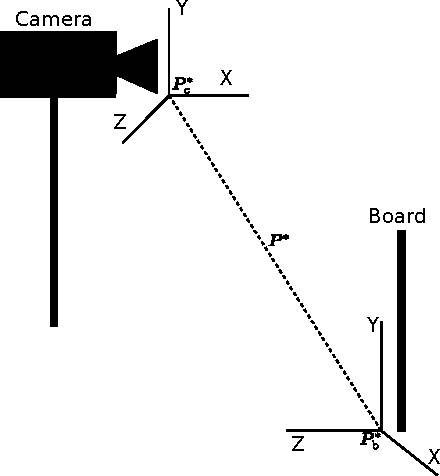
\includegraphics[width=0.8\textwidth]{figures/chapter3/P_star}
    \caption{Diagram showing the relation between the pose vector between the camera and board within the Vicon axis system.}
    \label{fig:chap3-p-star}
  \end{subfigure}
  ~
  \begin{subfigure}[t]{0.48\textwidth}
    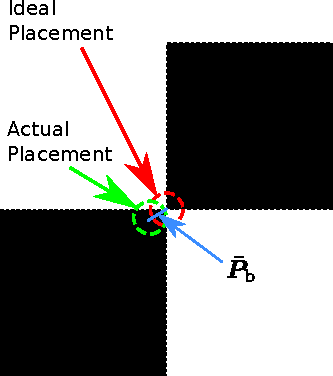
\includegraphics[width=0.7\textwidth]{figures/chapter3/P_bar}
    \caption{Diagram showing the marker placement error offset in the calibration board. }
    \label{fig:chap3-p-bar}
  \end{subfigure}
\caption{Diagrams showing the relationships between the pose vectors given by the Vicon and CVS.}
\end{figure*}

The equation for the pose estimate from the CVS is given by

\begin{equation}
  \label{eq:chap3-cvs}
  \bm{P}(f_x, f_y) = \bm{P}^* - \bar{\bm{P}} + \bm{\epsilon}.
\end{equation}
Equation~\ref{eq:chap3-cvs} indicates that the CVS's pose measurements, $\bm{P}(f_x, f_y)$, are given by the Vicon's measurement ($\bm{P}^* - \bar{\bm{P}}$) plus some error vector, $\bm{\epsilon}$, which represents the CVS's measurement error. Equation~\ref{eq:chap3-cvs} can be simplified to the form given in Equation~\ref{eq:chap3-pose}, which forms the basis of the optimisation algorithm moving forward.  

\begin{equation}
  \label{eq:chap3-pose}
  \bm{P}(f_x, f_y) = (\bm{P}^*_\mathrm{b} - \bar{\bm{P}}_\mathrm{b}) - (\bm{P}^*_\mathrm{c} - \bar{\bm{P}}_\mathrm{c}) + \bm{\epsilon}
\end{equation}
The next step is then to determine the constant perceived offset for a given focal length combination. The focal length is initialised with the focal lengths found during calibration (approximately 700 pixel units). By summing the samples, the offset, $\bm{\bar{P}}$, can be determined with  

\begin{equation}
  \label{eq:chap3-eq1-offset}
  M\bar{\bm{P}} = \sum\limits_{i=1}^M \bm{P}_i(f_x, f_y) - \sum\limits_{i=1}^M(\bm{P}^*_{\mathrm{b},i} - \bm{P}^*_{\mathrm{c}, i}) + \sum\limits_{i=1}^M\bm{\epsilon}_i.
\end{equation}
In Equation~\ref{eq:chap3-eq1-offset}, $i$ is the pose vector sample number and $M$ represents the number of samples in the data set. At this point, it is assumed that the error vector, $\bm{\epsilon}$, has a mean of zero, eliminating its sum and leading to Equation~\ref{eq:chap3-eq2-offset}. This assumption was made in the hope that the CVS will on average produce a small error and it is verified in Section~\ref{sec:err-norm-test}. 

\begin{equation}
  \label{eq:chap3-eq2-offset}
  \bar{\bm{P}} = \frac{1}{M} \left (\sum\limits_{i=1}^M \bm{P}_i(f_x, f_y) - \sum\limits_{i=1}^M(\bm{P}^*_{\mathrm{b},i} - \bm{P}^*_{\mathrm{c}, i})\right)
\end{equation}
Using the constant $\bar{\bm{P}}$ produced by Equation~\ref{eq:chap3-eq2-offset}, it is now possible to minimise the error vector, $\bm{\epsilon}$, of Equation~\ref{eq:chap3-pose} by varying the focal lengths, $f_x$ and $f_y$. The minimum focal lengths were found by setting up a $3\times n$ cell error matrix, consisting of the three translation dimensions, ${[x\;y\;z]}^T$, where $n$ is the number of samples in the data set, and find the optimal focal length combination by minimising the matrix's two-norm. The optimisation is based only on the three position dimensions since it was found that the orientation dimensions contain a large amount of noise and including them in the optimisation added too much variability to the procedure, leading to instability. Figure~\ref{fig:chap3-bad-optimisation} demonstrates this by comparing two images taken during the Vicon test: one using the optimum focal length calculated using only the position dimensions and the other using all six dimensions. 

\begin{figure*}
  \begin{subfigure}[t]{0.48\textwidth}
    \centering
    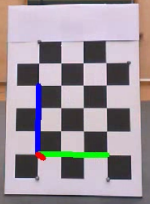
\includegraphics[width=0.7\textwidth]{figures/chapter3/3_dim_optimisation}
    \caption{Axis system drawn with focal length calculated from using the position dimensions.}
  \end{subfigure}
  ~
  \begin{subfigure}[t]{0.48\textwidth}
    \centering
    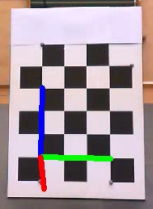
\includegraphics[width=0.7\textwidth]{figures/chapter3/6_dim_optimisation}
    \caption{Axis system drawn with focal length calculated from using all six dimensions.}
  \end{subfigure}
  \caption{Images demonstrating the optimisation procedure's sensitivity to the orientation dimensions.}
  \label{fig:chap3-bad-optimisation}
\end{figure*}

In Figure~\ref{fig:chap3-bad-optimisation}, the CVS drew axes onto the calibration board by using the pose it calculated. It can be seen that the axes differ from one another, indicating that the optimisation is sensitive when using the orientation dimensions in the optimisation procedure. 

The error matrix is produced by

\begin{equation}
  \label{eq:chap3-error-base}
  \bm{\epsilon} = \bm{P}(f_x, f_y) - \bm{P}^* - \bar{\bm{P}}.
\end{equation}
Using the $3\times n$ error matrix from Equation~\ref{eq:chap3-error-base}, an error vector is generated by summing the error matrix along its columns. The optimum focal lengths were then found by taking the focal length combination that produces the smallest two-norm of the sample error vector $\bm{\epsilon}$. The minimisation equation is given by 

\begin{equation}
  \label{eq:chap3-err-min}
  \min_{\hat{f}_x, \hat{f}_y}\left \Vert \sum_i  \bm{\epsilon}_i \right \Vert,
\end{equation}
where $\hat{f}_x$ and $\hat{f}_y$ refer to the optimum focal lengths. With the optimal focal length now determined, the procedure is repeated again from Equation~\ref{eq:chap3-pose}, finding a new offset for the new focal length combination. The optimisation procedure is iterated a number of times, minimising the total error norm. After the optimum focal length combination was found, that combination was used in the camera matrix that extracted the pose data from the video data.

The optimisation procedure is summarised in Algorithm~\ref{alg:optimal}. 

\begin{algorithm}
  \centering
  \caption{Optimise Camera Focal Length Parameter}
  \label{alg:optimal}
  \begin{algorithmic}
    \State Initialise variables: 
      \State $\hat{f}_x \gets 700.0$
      \State $\hat{f}_y \gets 700.0$
      \State $i \gets 0$
      \While{$\left \Vert \bm{\epsilon} \right \Vert > \left \Vert \bm{\epsilon}_{min} \right \Vert$}
      \State Find $\bm{\bar{P}}$ for $f_x^i$ and $f_y^i$ (Equation~\ref{eq:chap3-eq2-offset})
      \State Determine $\left \Vert \hat{\bm{\epsilon}} \right \Vert$ for the new $\bm{\bar{P}}$ (Equation~\ref{eq:chap3-error-base})
      \If{$\left \Vert \hat{\bm{\epsilon}} \right \Vert < \left \Vert \bm{\epsilon} \right \Vert$}
        \State $\bm{\epsilon} \gets \hat{\bm{\epsilon}}$
	\State $\hat{f}_x \gets f_x^i$
	\State $\hat{f}_y \gets f_y^i$
      \EndIf
      \State $i \gets i + 1$
    \EndWhile
    \State $\hat{\bm{P}} \gets \bm{P}(\hat{f}_x, \hat{f}_y)$
  \end{algorithmic}
\end{algorithm}

\section{Results}

Several sets of data were produced during the data processing phase. The results are presented and discussed in this section. They include evidence of error convergence for the optimisation procedure, as well as proofs that the error $\bm{\epsilon}$ is indeed distributed around zero and also roughly normally distributed. Lastly, the new focal length combination is given and discussed, followed by the pose measurement accuracy results of the CVS. 

\subsection{Evidence of Convergence}

To show that the optimisation procedure worked as expected, minimising the error in each dimension, the error after each iteration of the process is plotted. These plots are given in Figure~\ref{fig:err-convergence} and shows the error over 15 iterations of the optimisation procedure.  

\begin{figure*}
  \centering
  \begin{subfigure}{0.48\textwidth}
    \begin{subfigure}{\textwidth}
      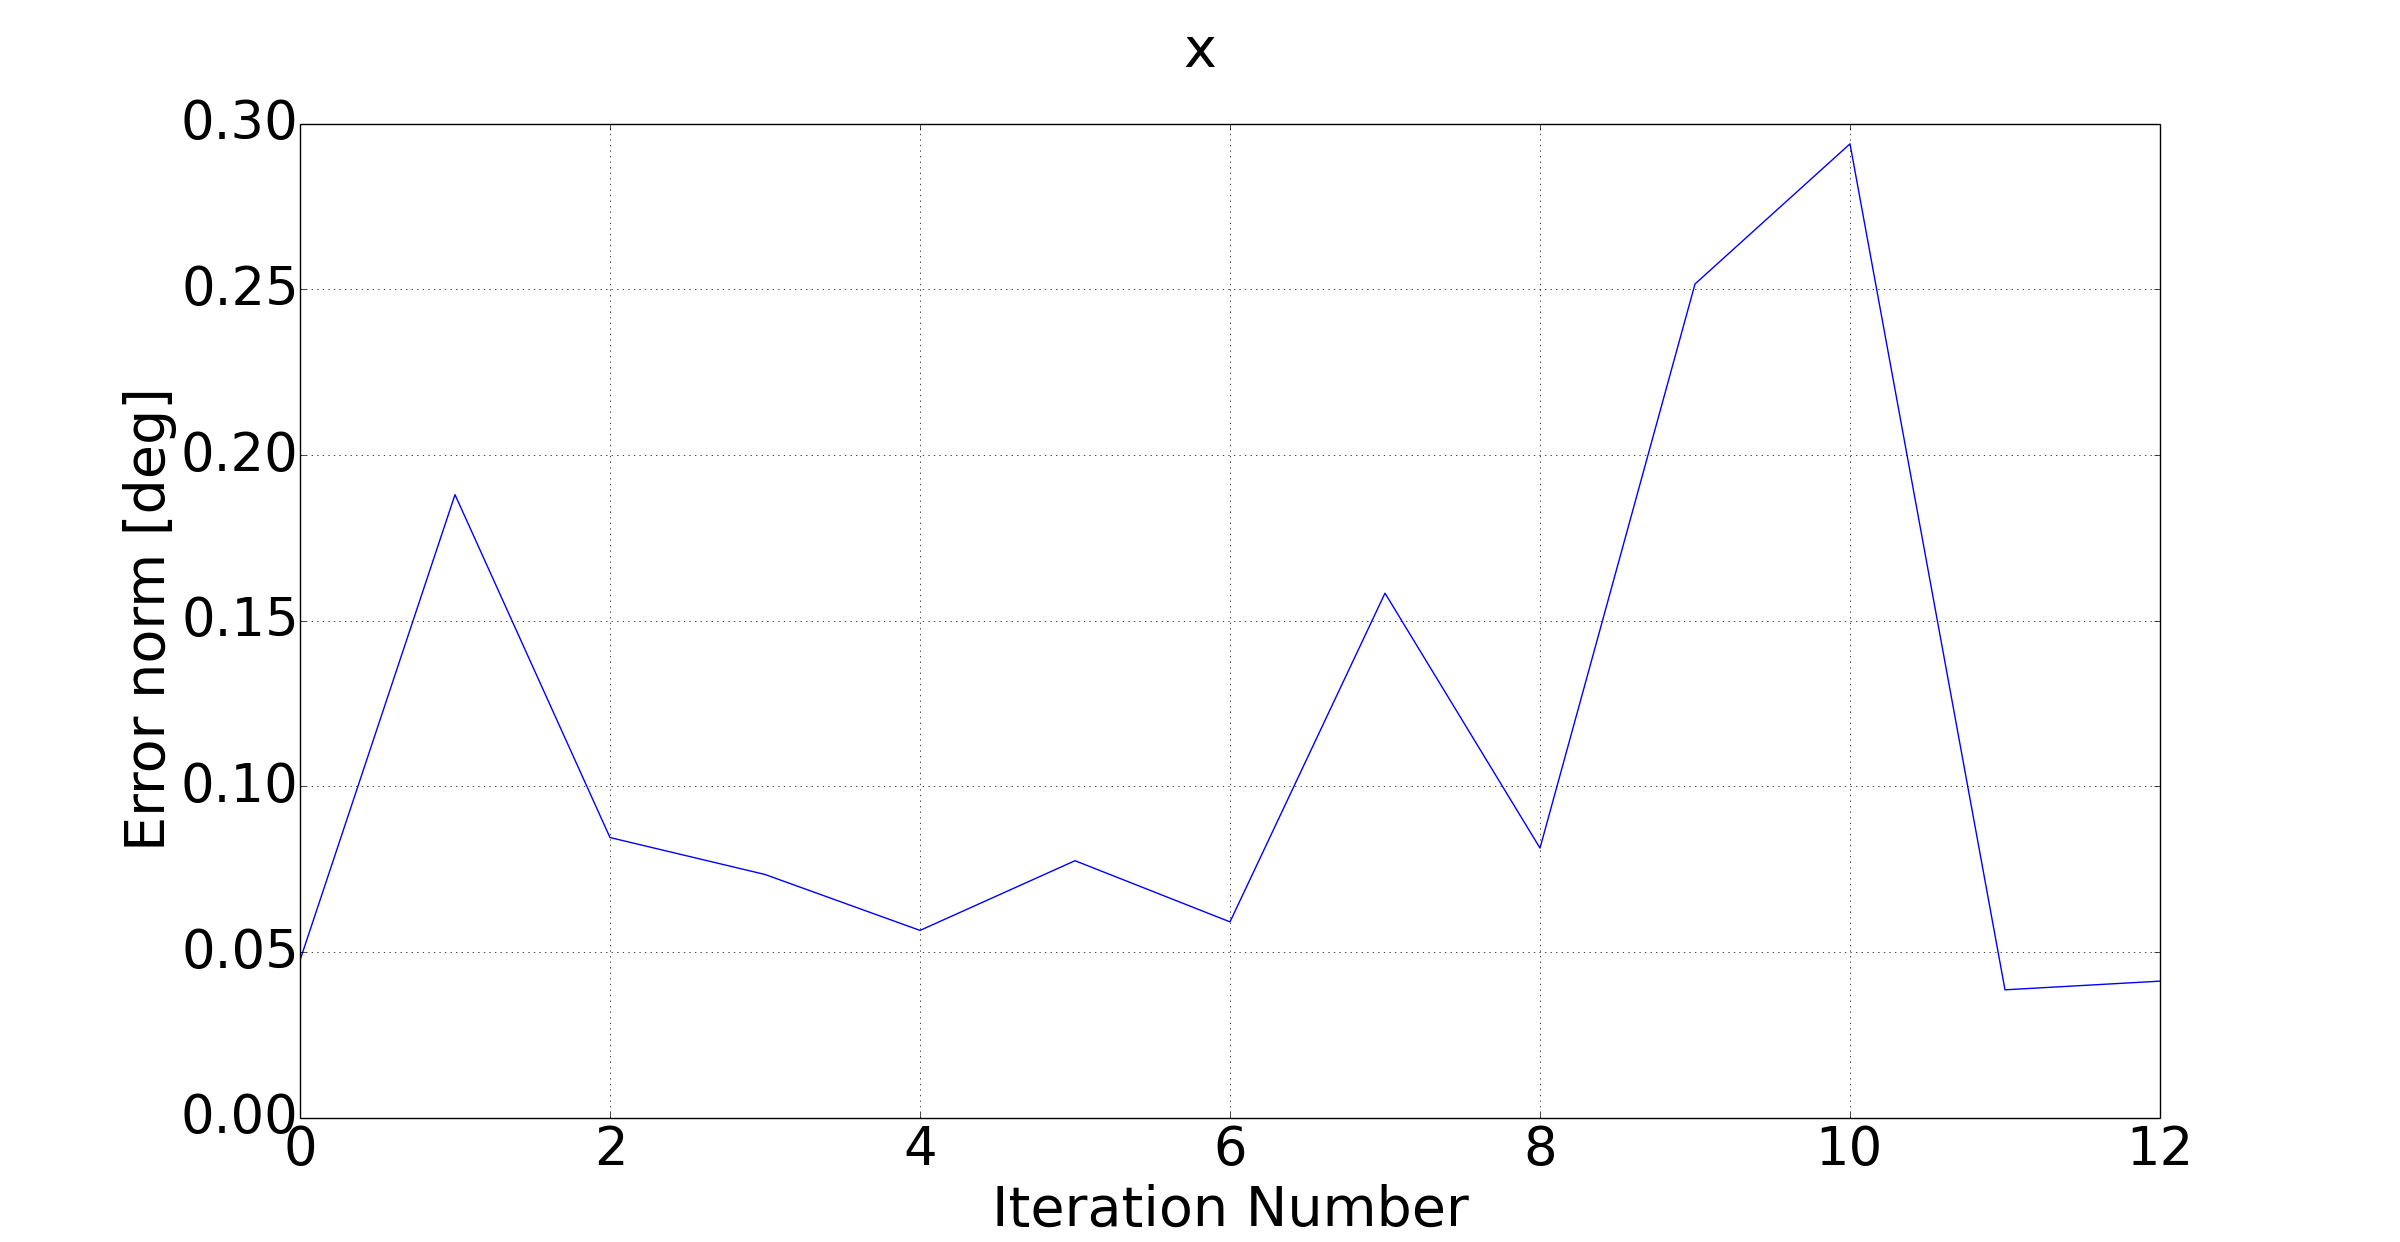
\includegraphics[clip, trim = 60 0 140 20, width=\textwidth]{figures/chapter3/err_x}
    \end{subfigure}
    \begin{subfigure}{\textwidth}
      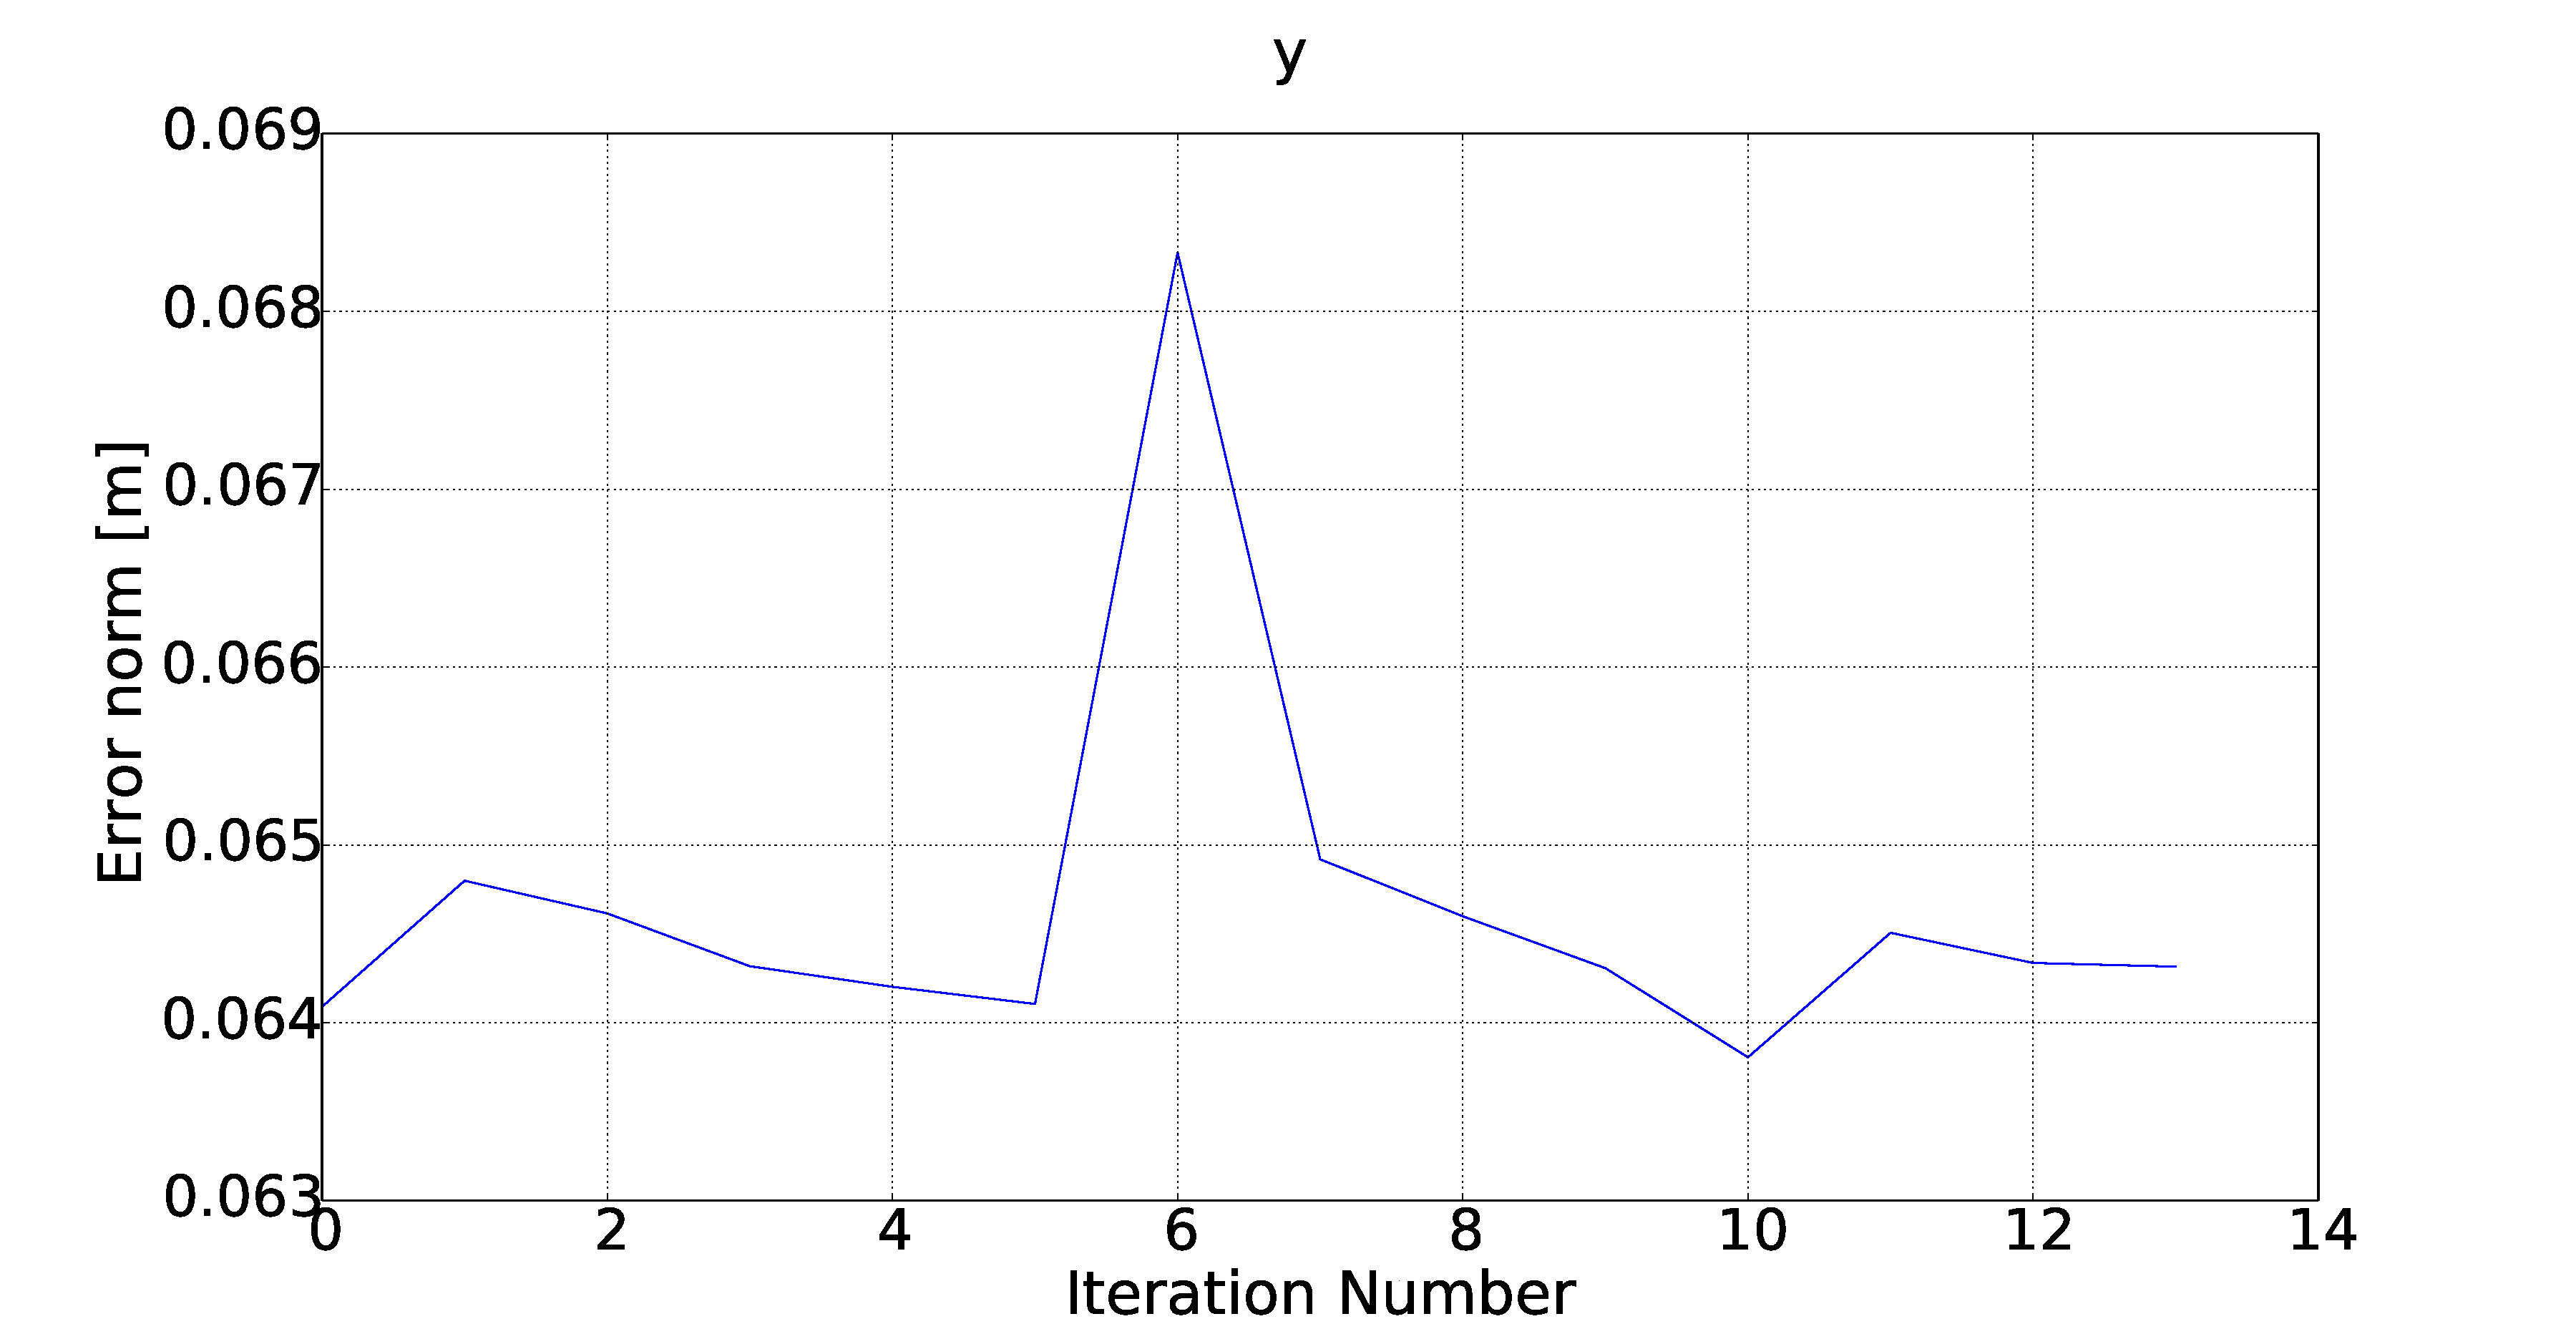
\includegraphics[clip, trim = 60 0 140 0, width=\textwidth]{figures/chapter3/err_y}
    \end{subfigure}
    \begin{subfigure}{\textwidth}
      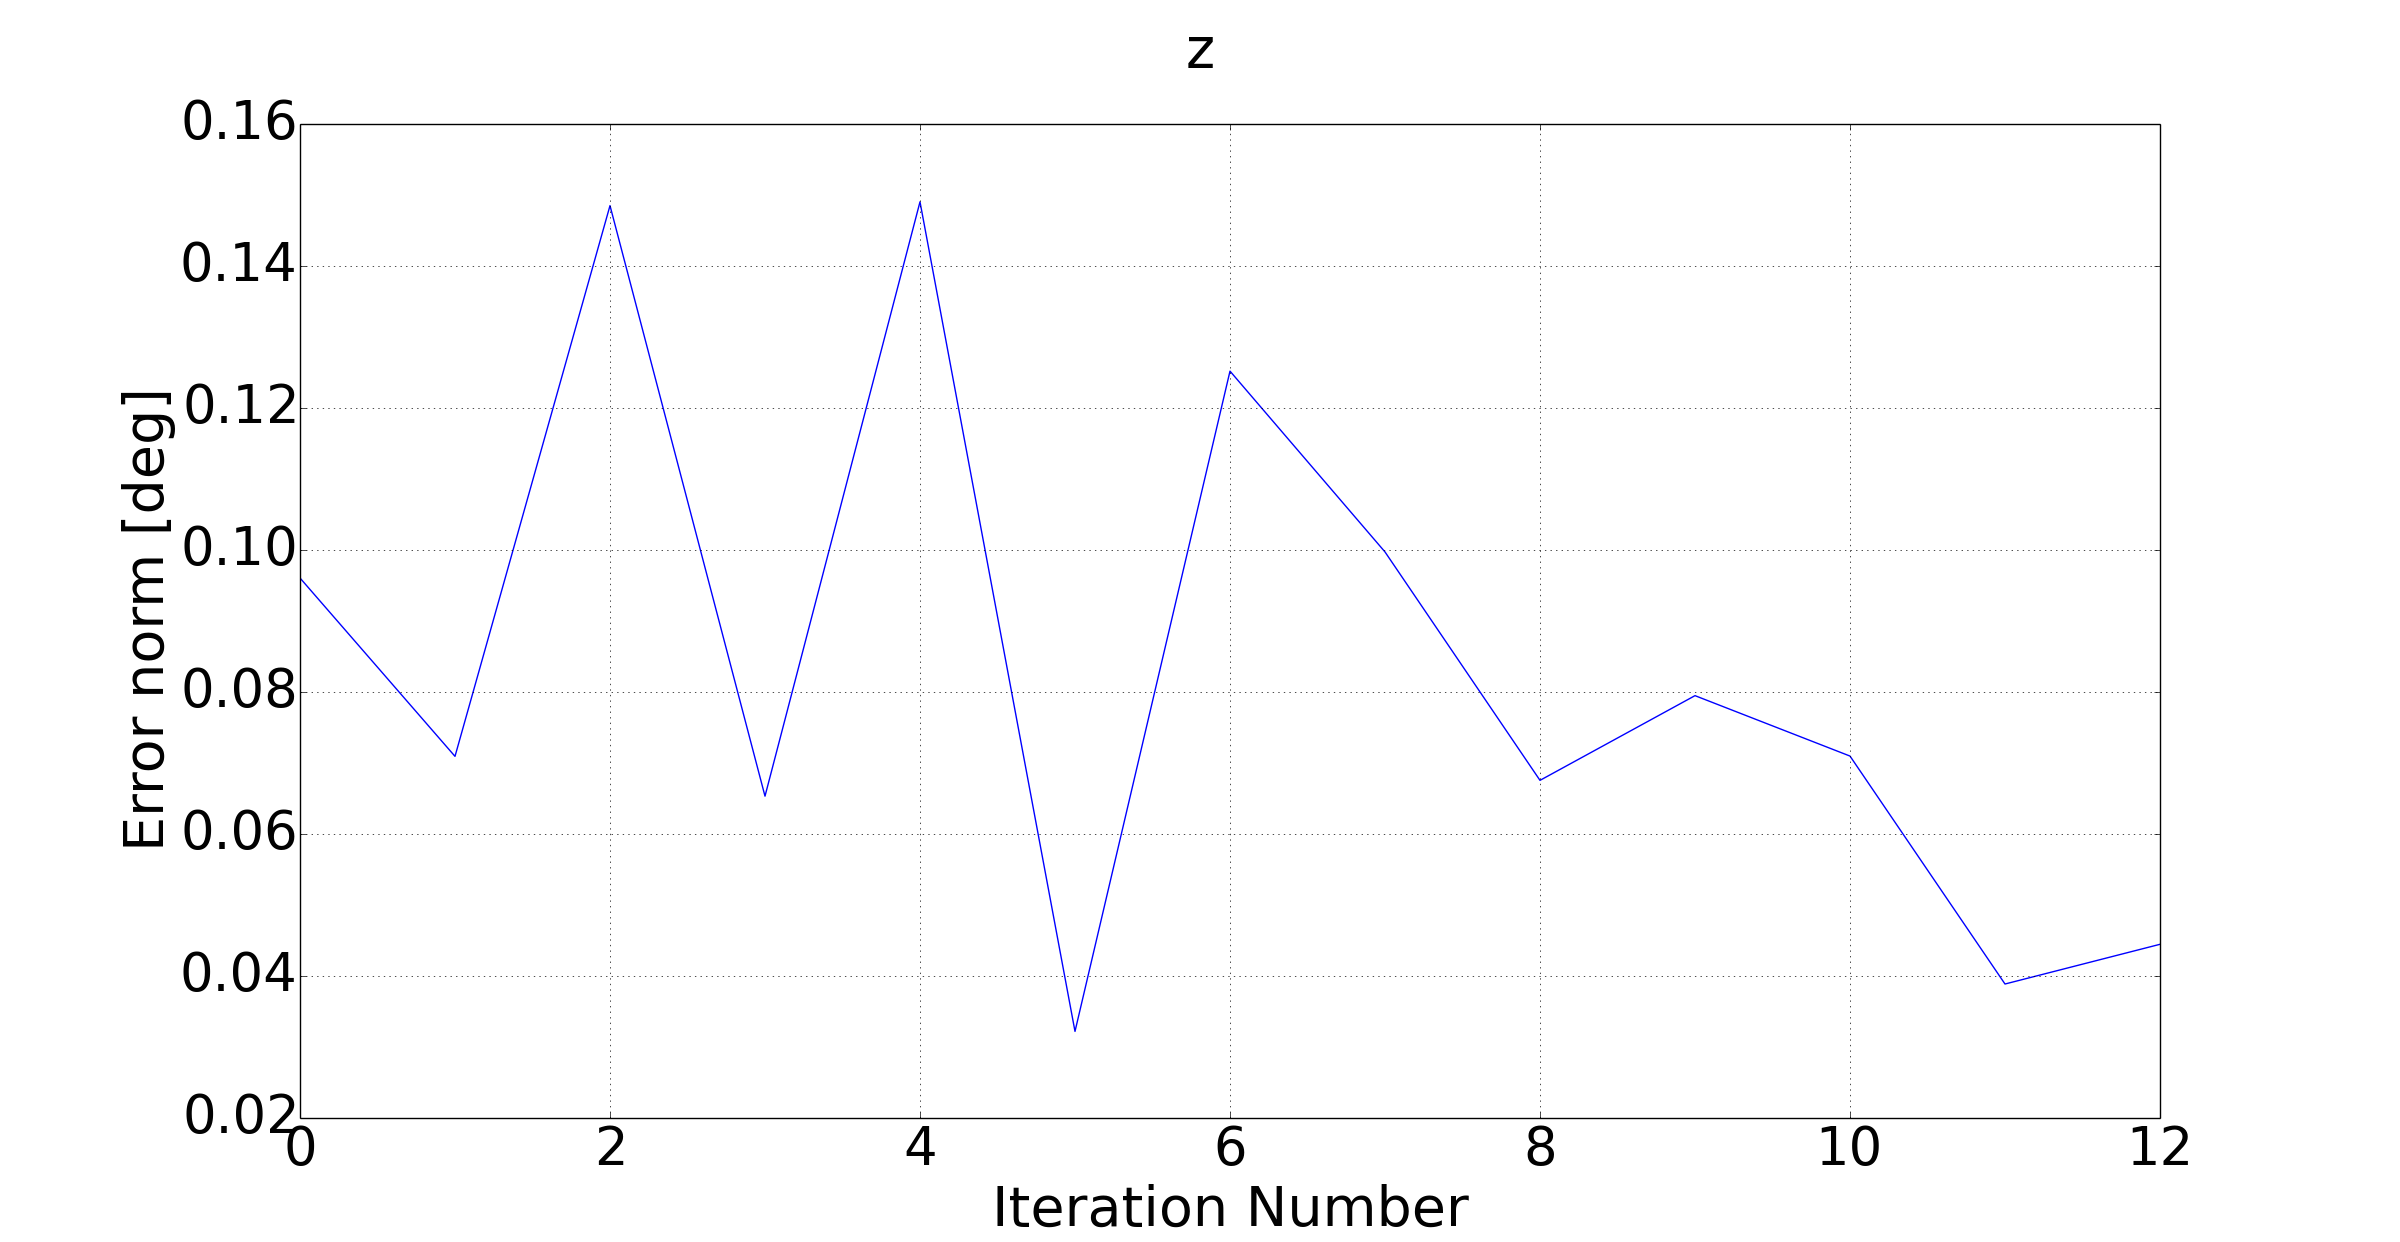
\includegraphics[clip, trim = 60 0 140 0, width=\textwidth]{figures/chapter3/err_z}
    \end{subfigure}
    \caption{Error convergence plots for the position dimensions.}
  \end{subfigure}
  ~
  \begin{subfigure}{0.48\textwidth}
    \begin{subfigure}{\textwidth}
      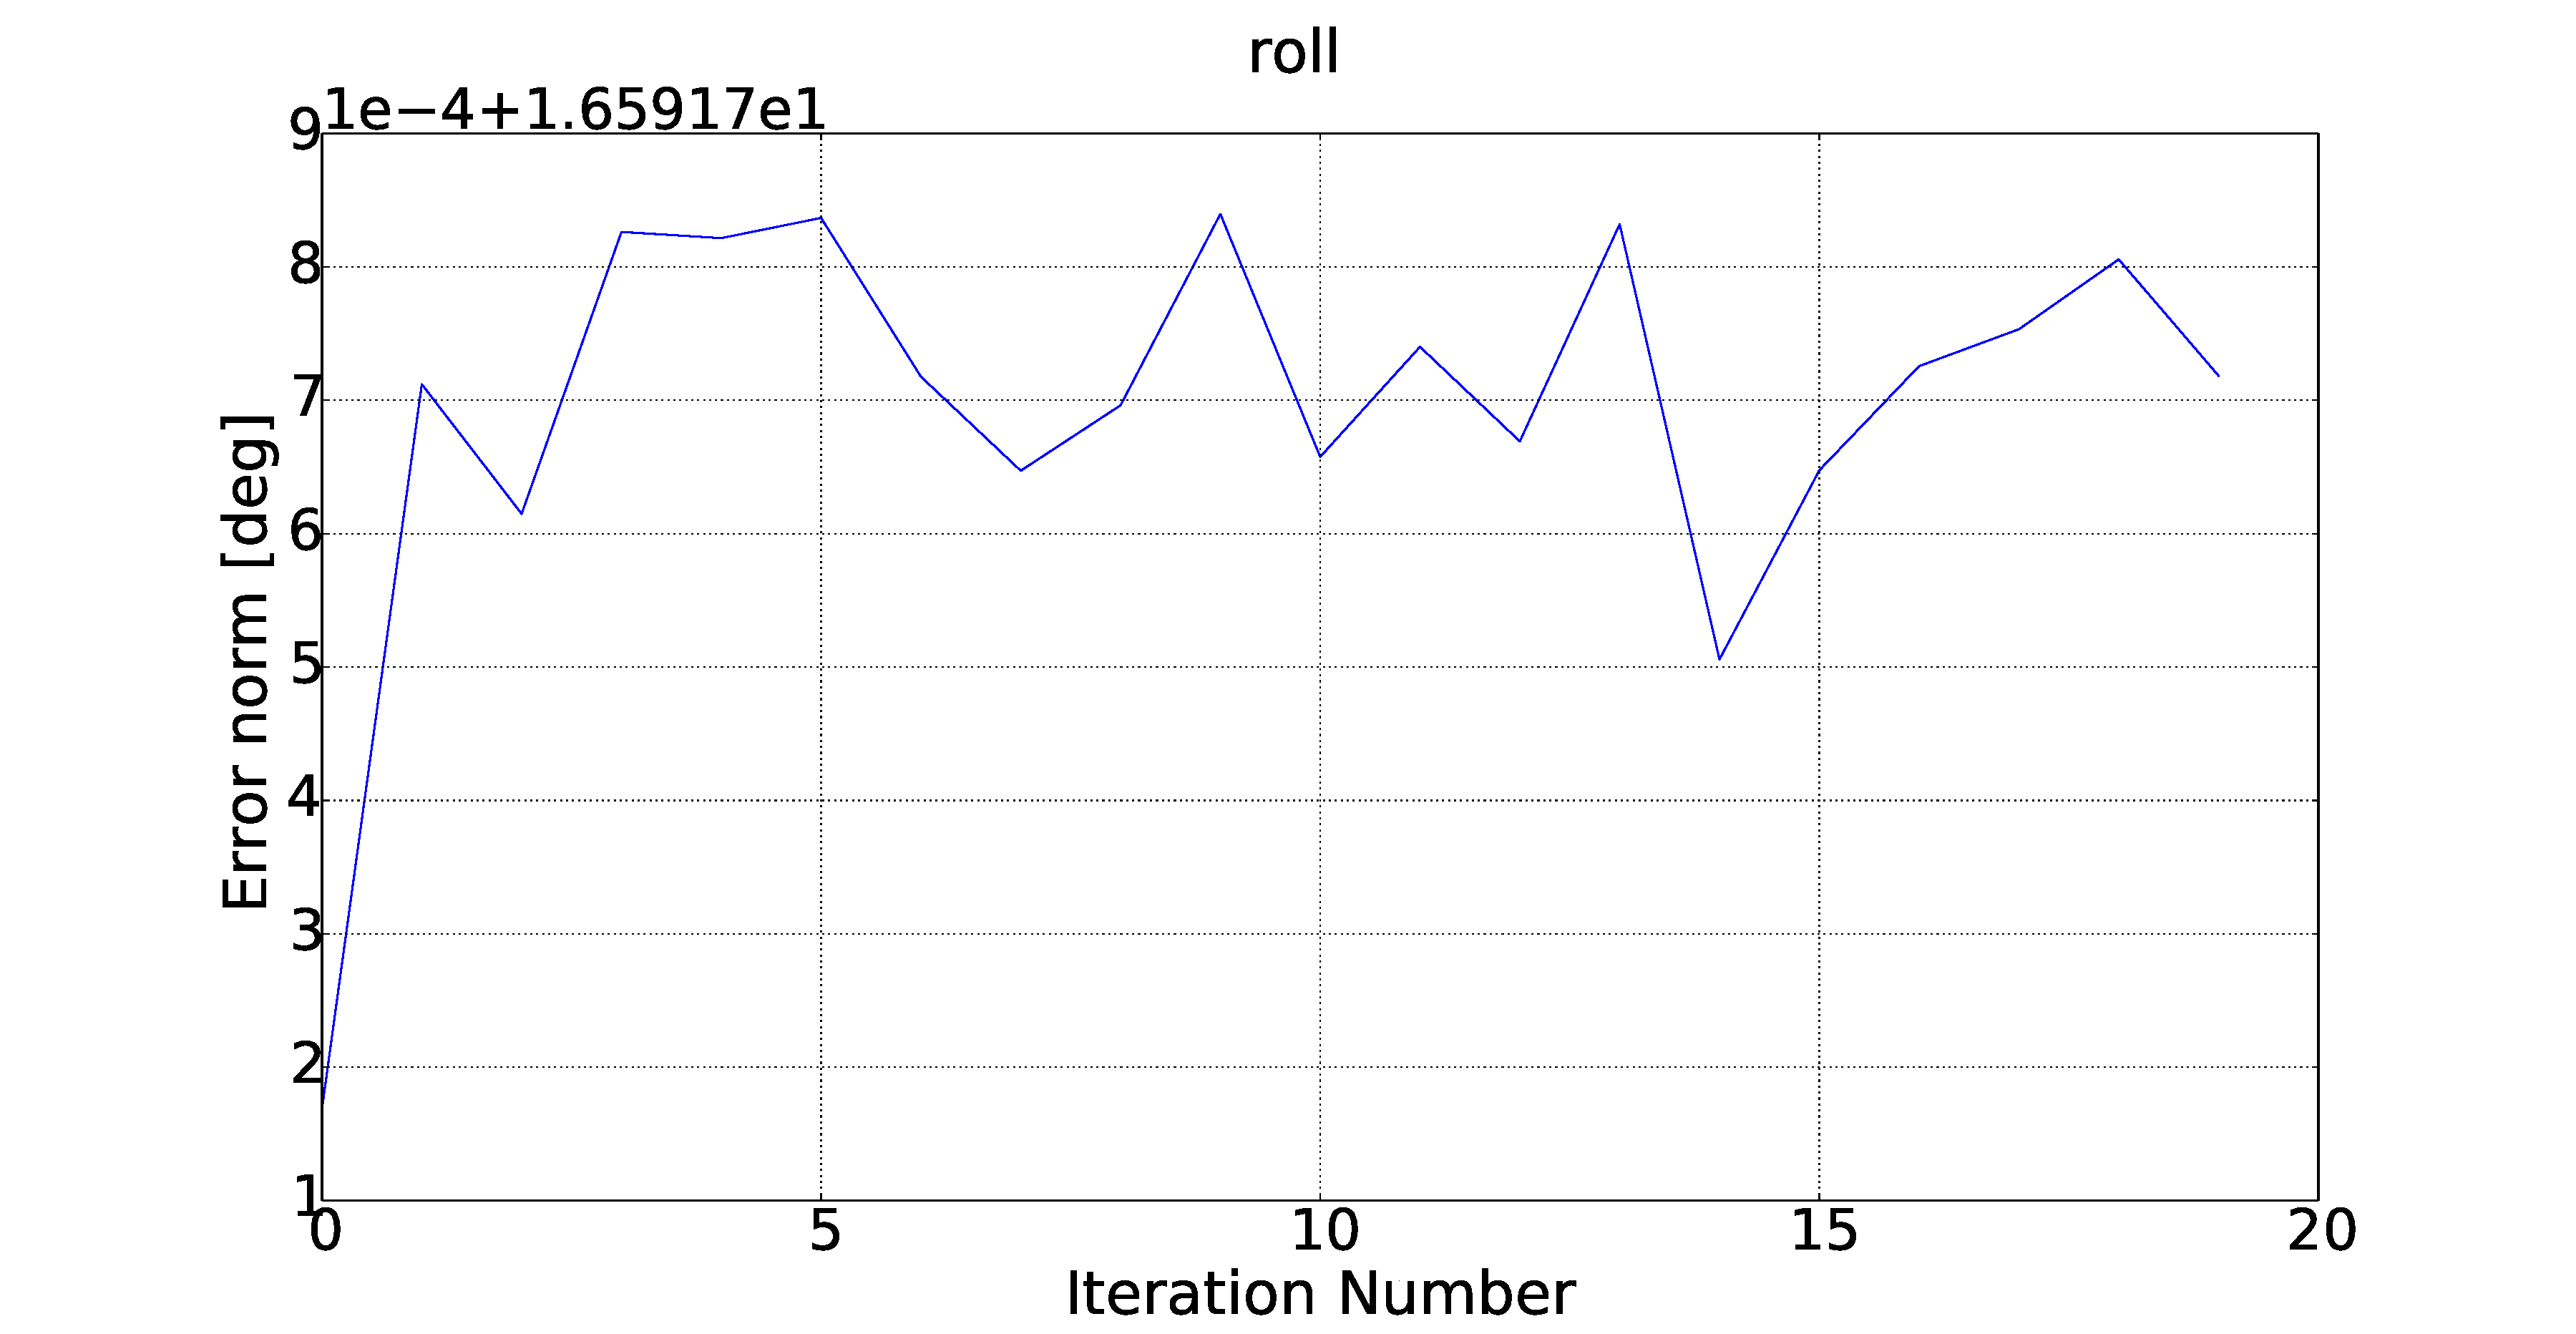
\includegraphics[clip, trim = 100 0 120 0, width=\textwidth]{figures/chapter3/err_roll}
    \end{subfigure}
    \begin{subfigure}{\textwidth}
      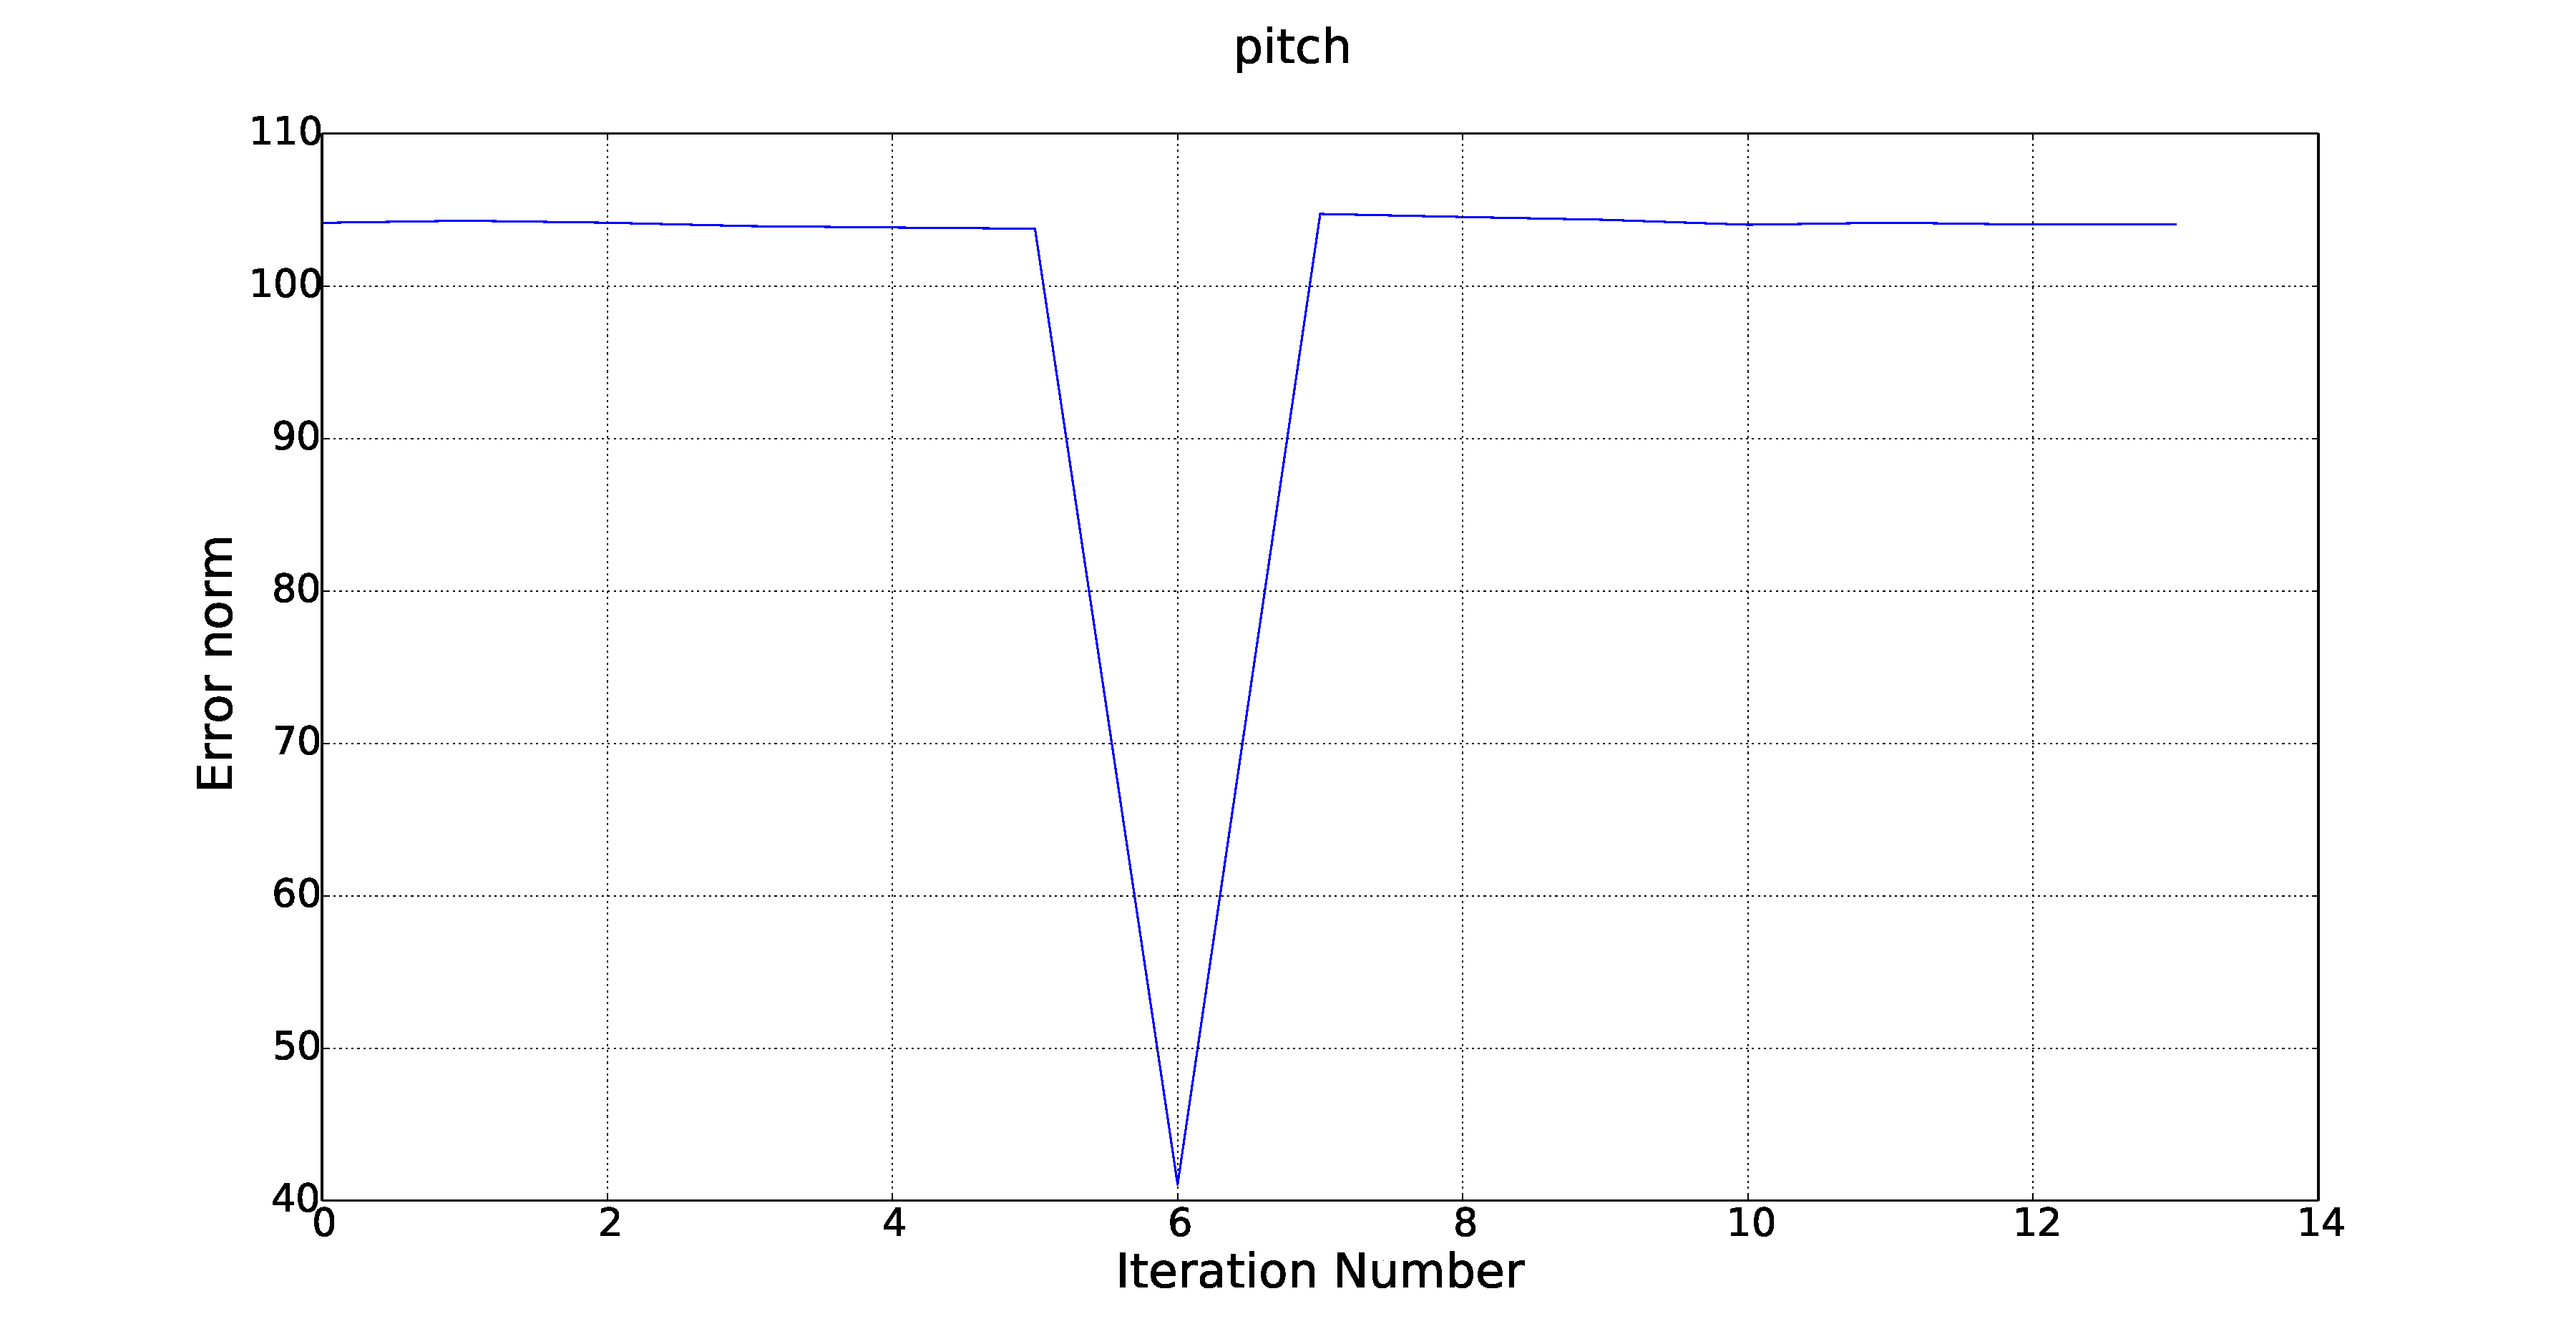
\includegraphics[clip, trim = 100 0 120 0, width=\textwidth]{figures/chapter3/err_pitch}
    \end{subfigure}
    \begin{subfigure}{\textwidth}
      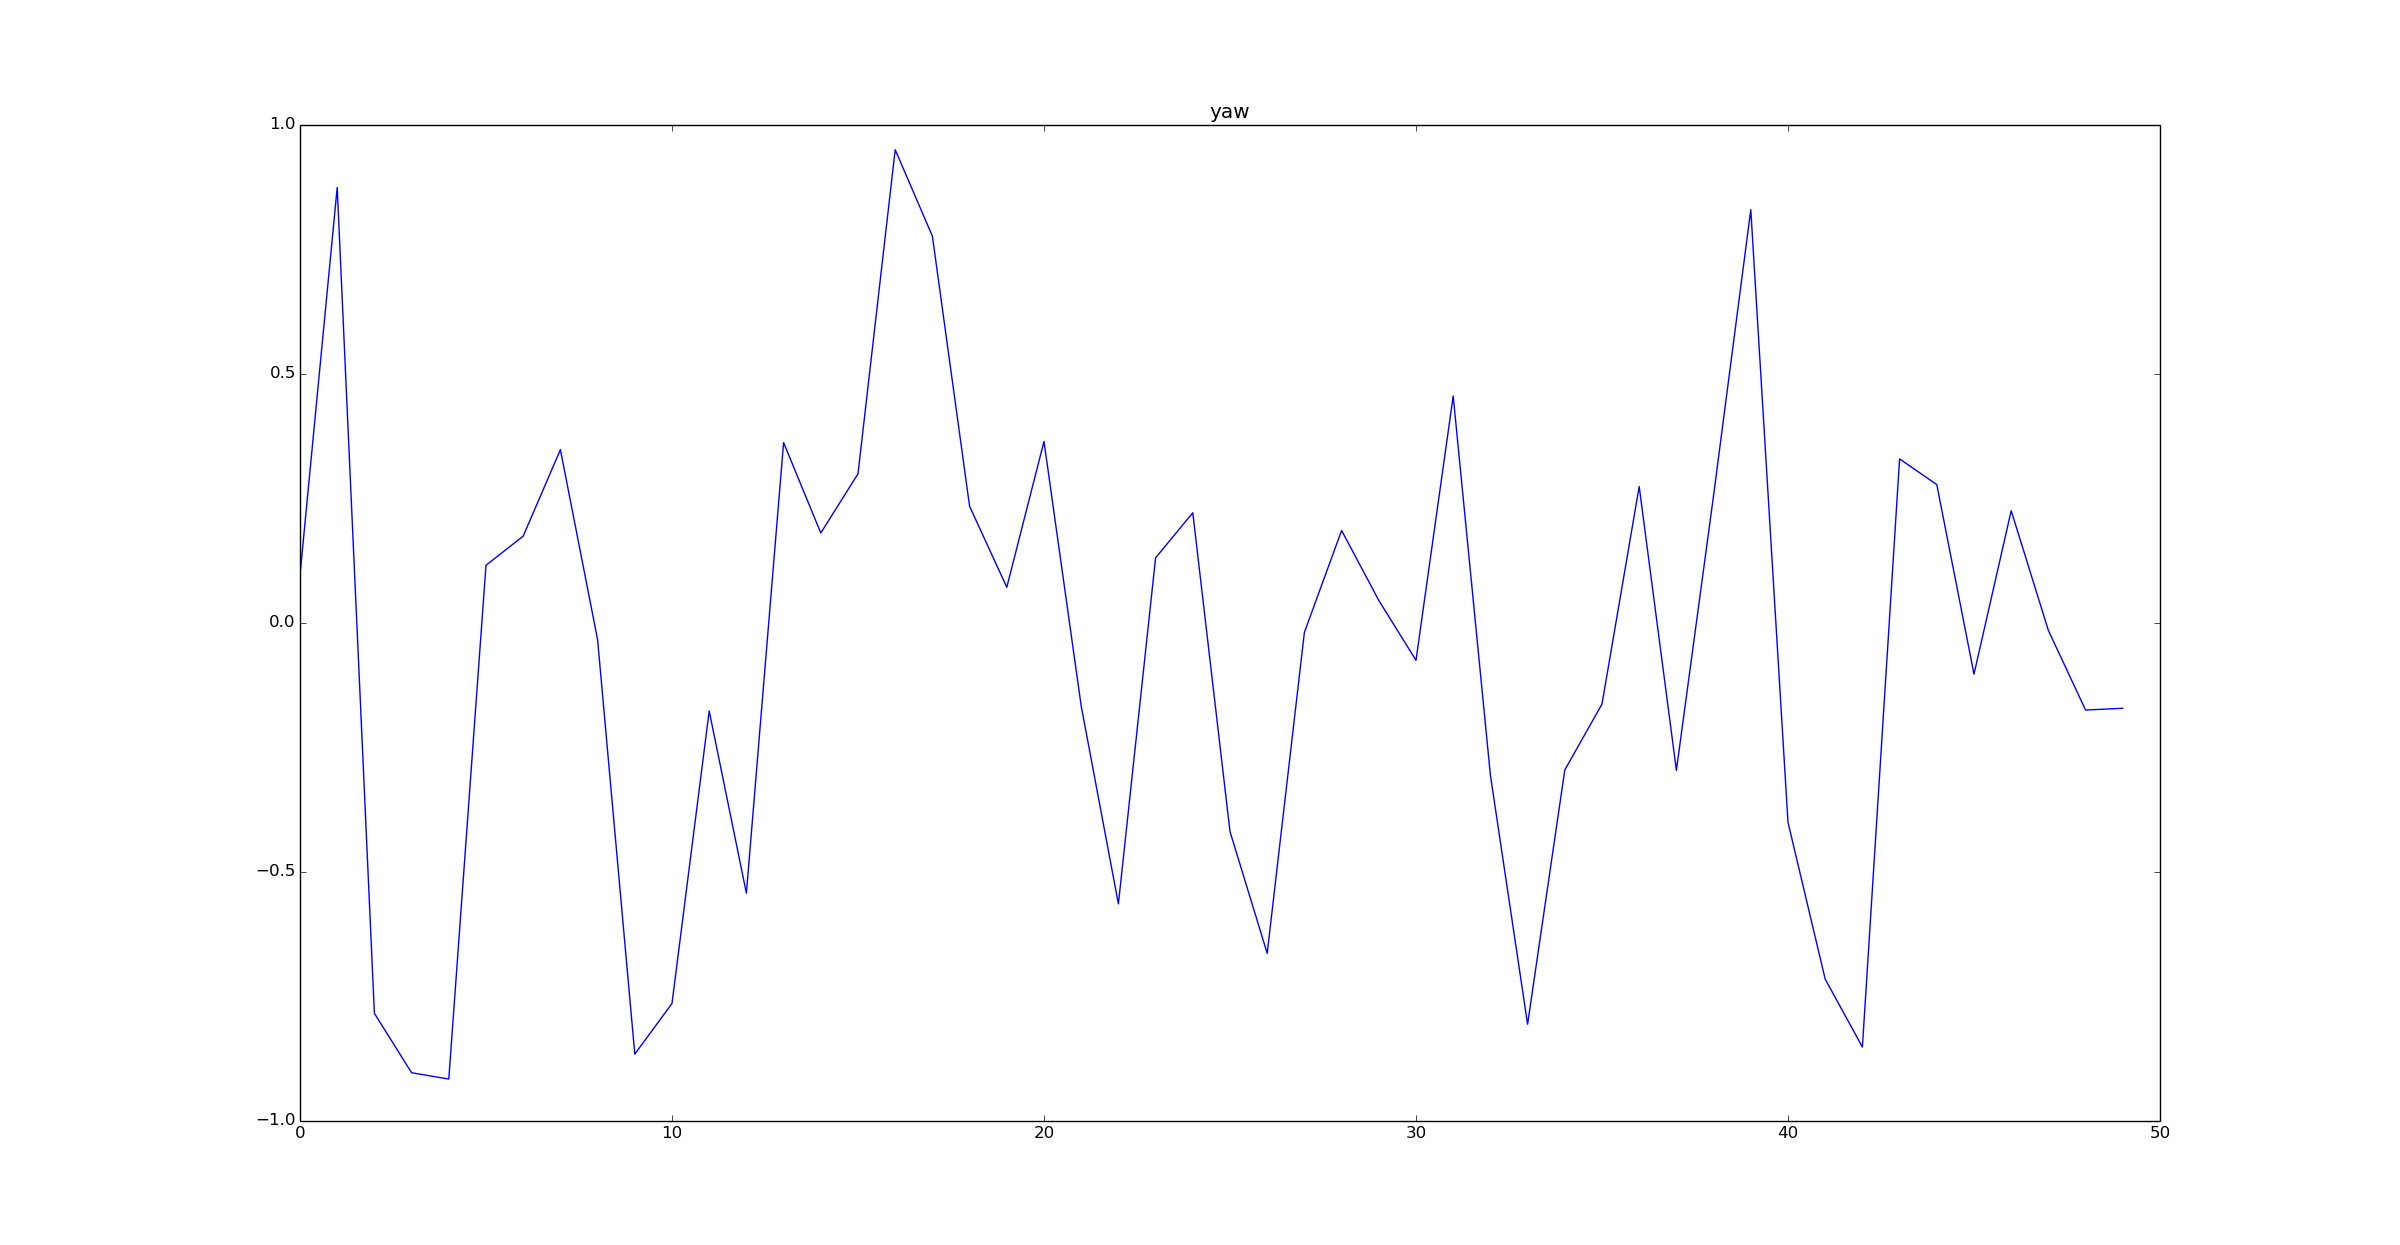
\includegraphics[clip, trim = 100 0 120 0, width=\textwidth]{figures/chapter3/err_yaw}
    \end{subfigure}
    \caption{Error convergence plots for the orientation dimensions.}
  \end{subfigure}
  \caption[Plots showing error convergence for the optimsation procedure.]{Plots showing the error in each dimension during for each iteration of the error minimisation procedure.}
  \label{fig:err-convergence}
\end{figure*}

The graphs of Figure~\ref{fig:err-convergence} show that the error is reduced in the $x$ and $z$ dimensions, while it increases slightly in the $y$ dimension and remains largely unchanged in all of the orientation dimensions. 

The errors in the orientation dimensions remain unchanged since it was opted not to give them any weight in the optimisation process. However, it can be seen that in iteration number 6, the $roll$, $pitch$ and $z$ dimensions experience a dramatic reduction in their error norm, while the other dimensions experience a spike. Since it happens only for a single iteration, it can be considered an anomaly within the optimisation procedure which is corrected  with the next iteration. It is most likely that the error got stuck in a local minimum for that single iteration.  

From Figure~\ref{fig:err-convergence} it can be concluded that the optimisation procedure does indeed converge, albeit very slowly. 

\subsection{Test for Zero Average Error}
\label{sec:err-norm-test}

To verify whether the error in $\bm{\epsilon}$ is indeed distributed around a zero mean value as assumed in Equation~\ref{eq:chap3-eq2-offset}, a $\chi^2$ (chi-squared) test could have been used. However, it was found that the sample size of the data set was too large, where the large number of samples can mislead the $\chi^2$ test to believe the data contains skewness and it is known that skewness in the data can have a large impact on the $\chi^2$ probability estimate~\citep{wackerly2007mathematical}. Therefore, a graphical approach was taken. This was done by drawing frequency histograms of the error, $\bm{\epsilon}$, in all six dimensions, along with a normal distributions drawn using each dimension's mean and standard deviation. This is done to check if the error data is normally distributed, since this will allow additional tools to be used and justify future assumptions. The plots are given in Figure~\ref{fig:err-norm}.

\begin{figure*}
  \begin{subfigure}{0.48\textwidth}
    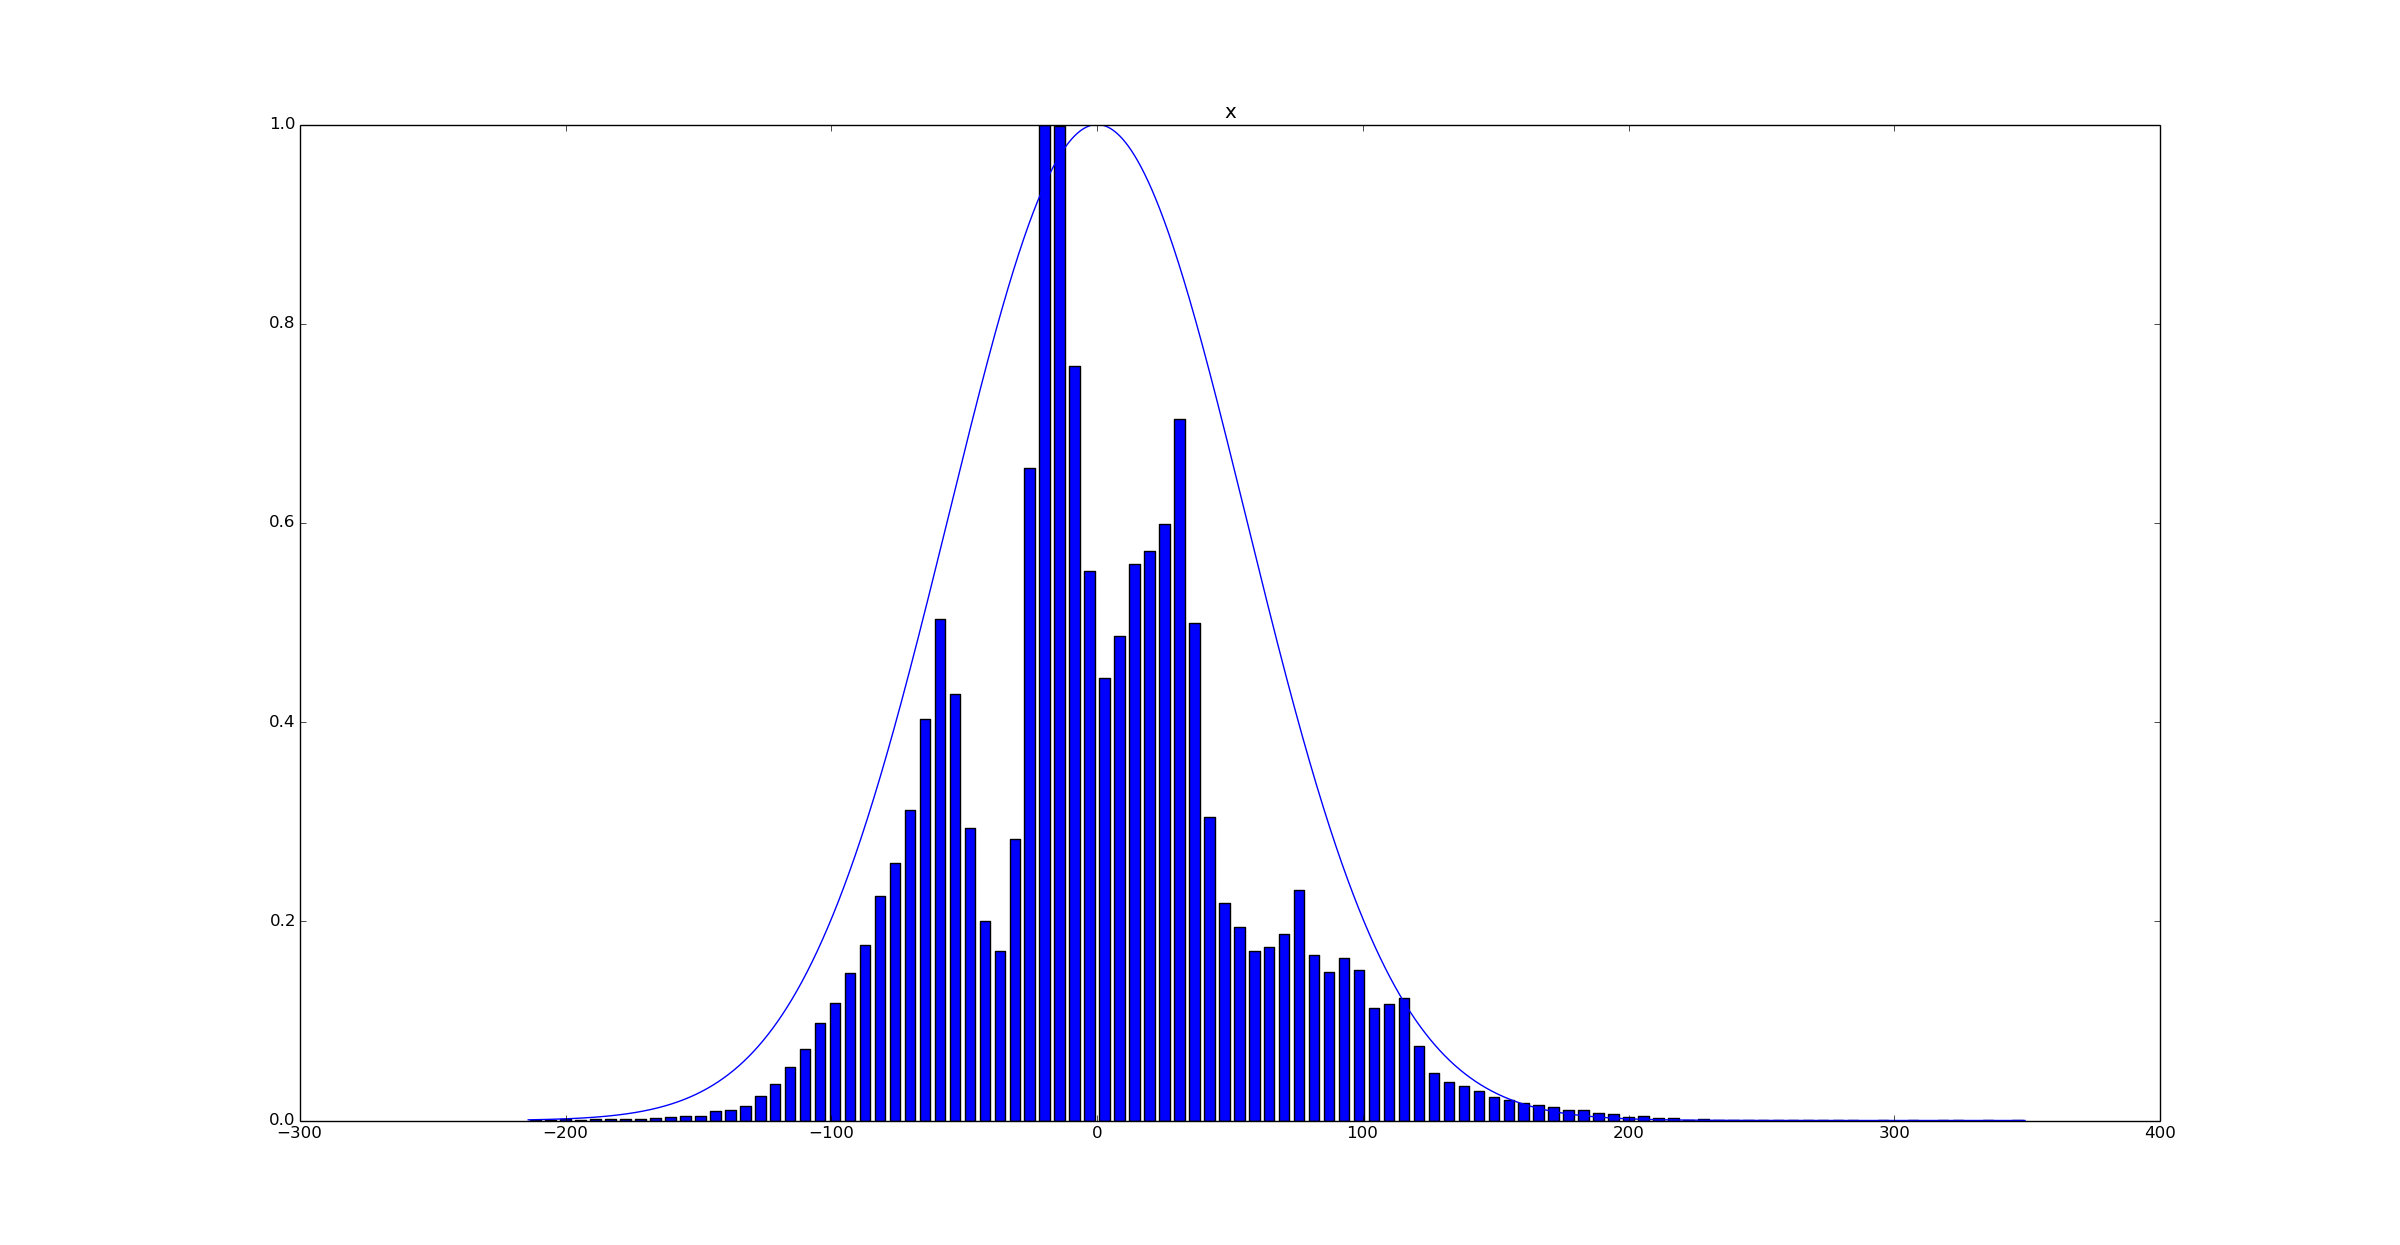
\includegraphics[clip, trim = 120 0 120 0, width=\textwidth]{figures/chapter3/norm_x}
    \caption{$\mu = \SI{-0.556}{\mm}$, $\sigma = \SI{32.5}{\mm}$.}
    \label{fig:chap3-err-norm-x}
  \end{subfigure}
~
  \begin{subfigure}{0.48\textwidth}
     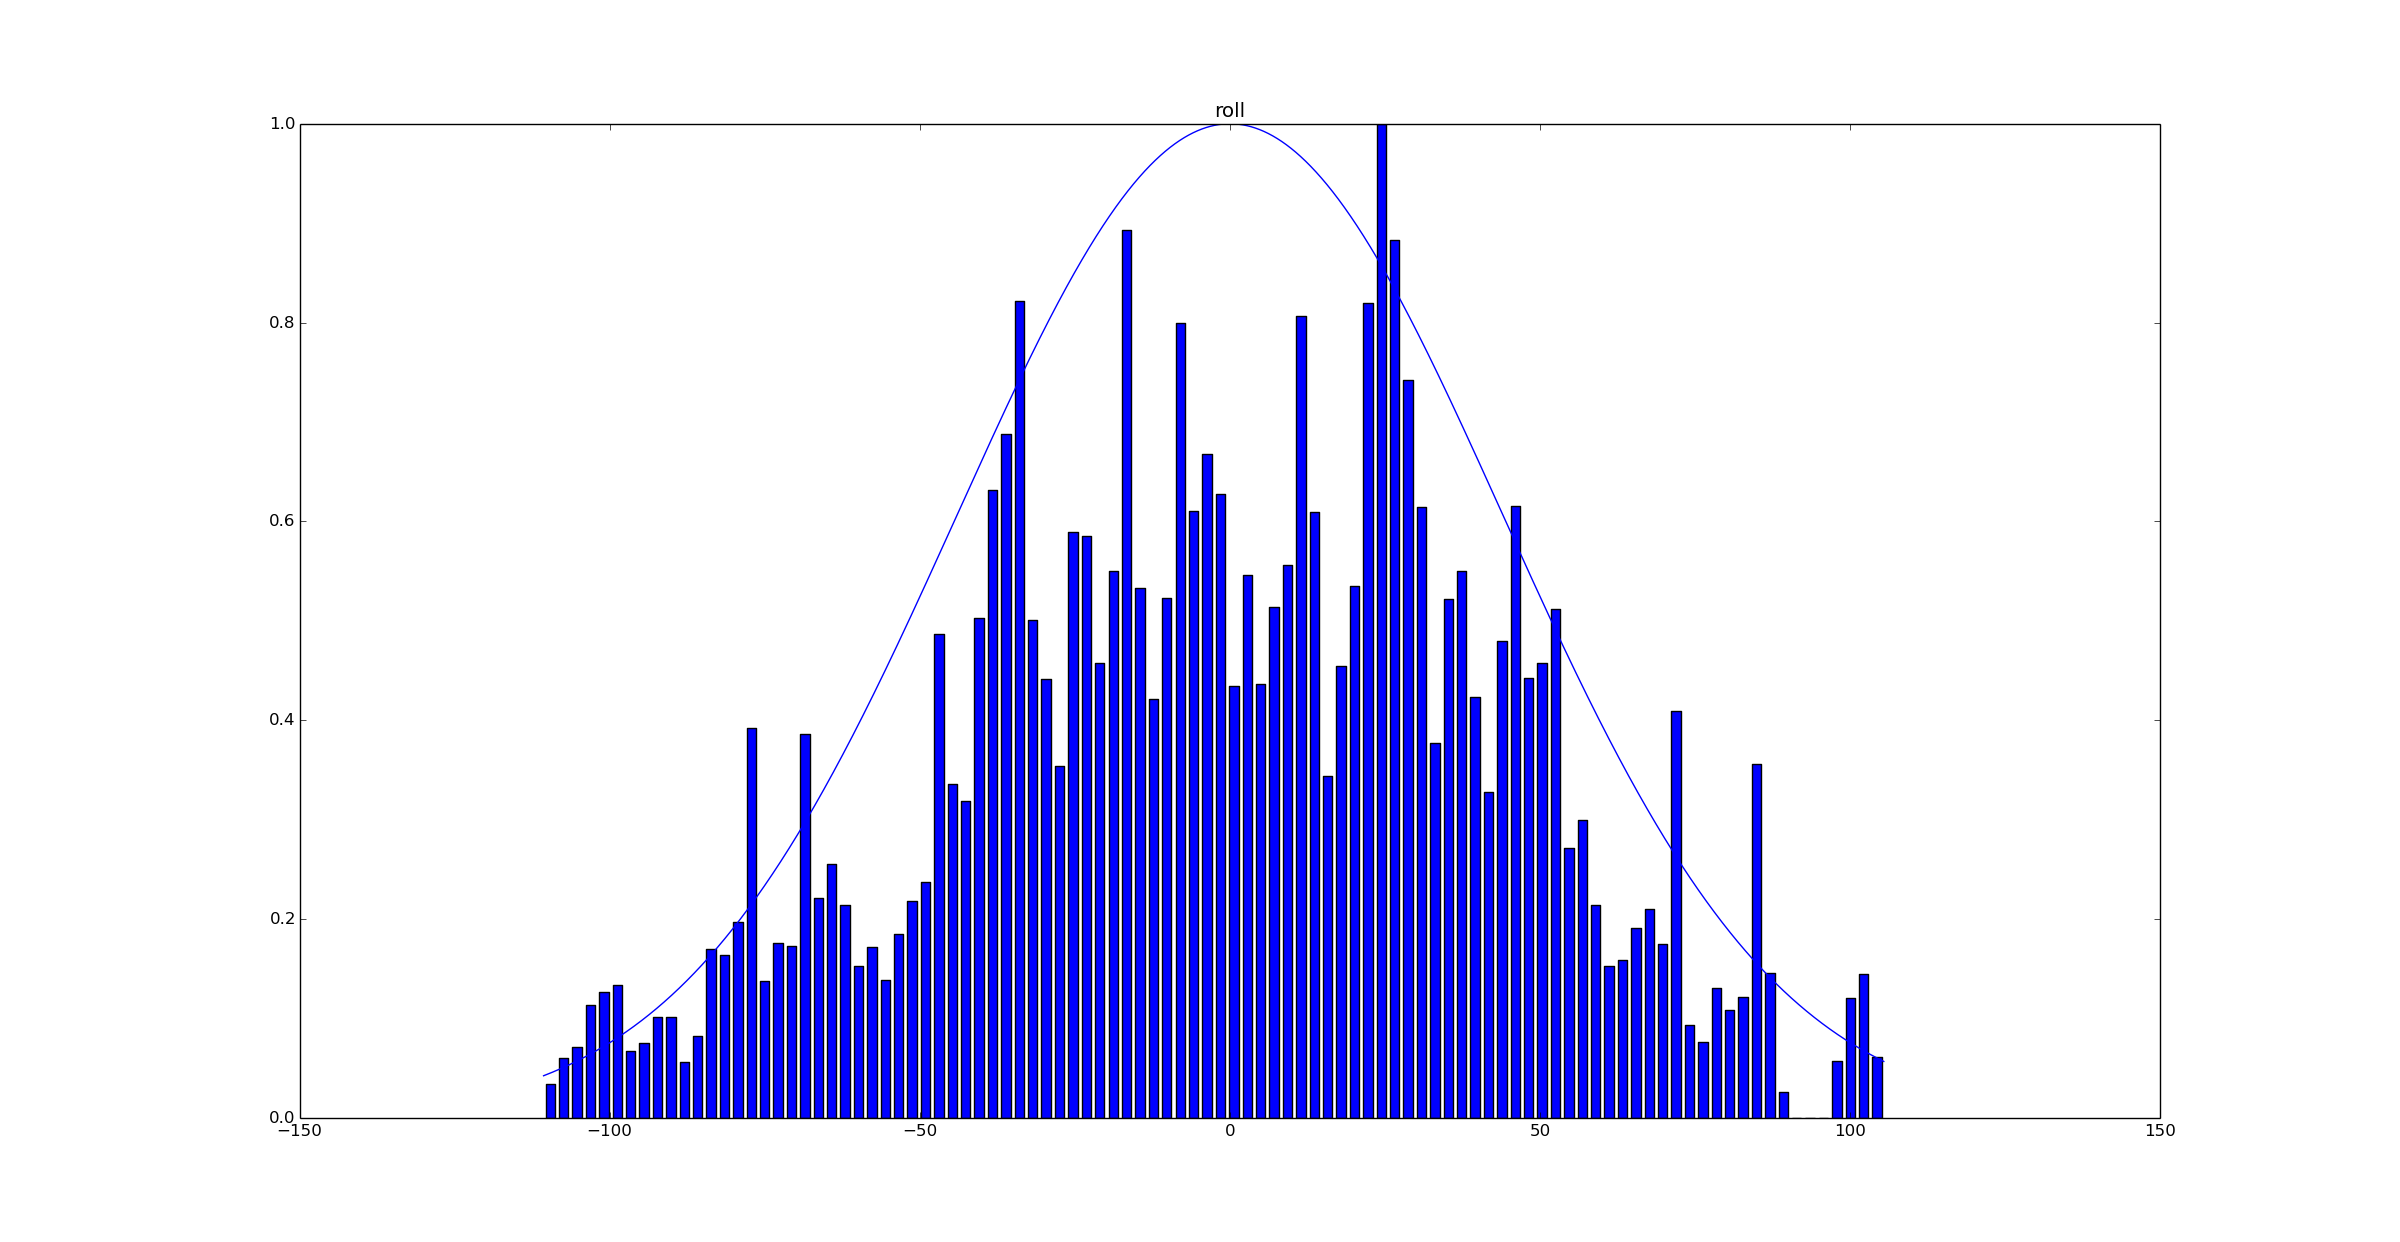
\includegraphics[clip, trim = 120 0 120 0, width=\textwidth]{figures/chapter3/norm_roll}
     \caption{$\mu = \ang{0.251}$, $\sigma = \ang{3.27}$.}
  \label{fig:norm-roll}
  \end{subfigure}

  \begin{subfigure}{0.48\textwidth}
     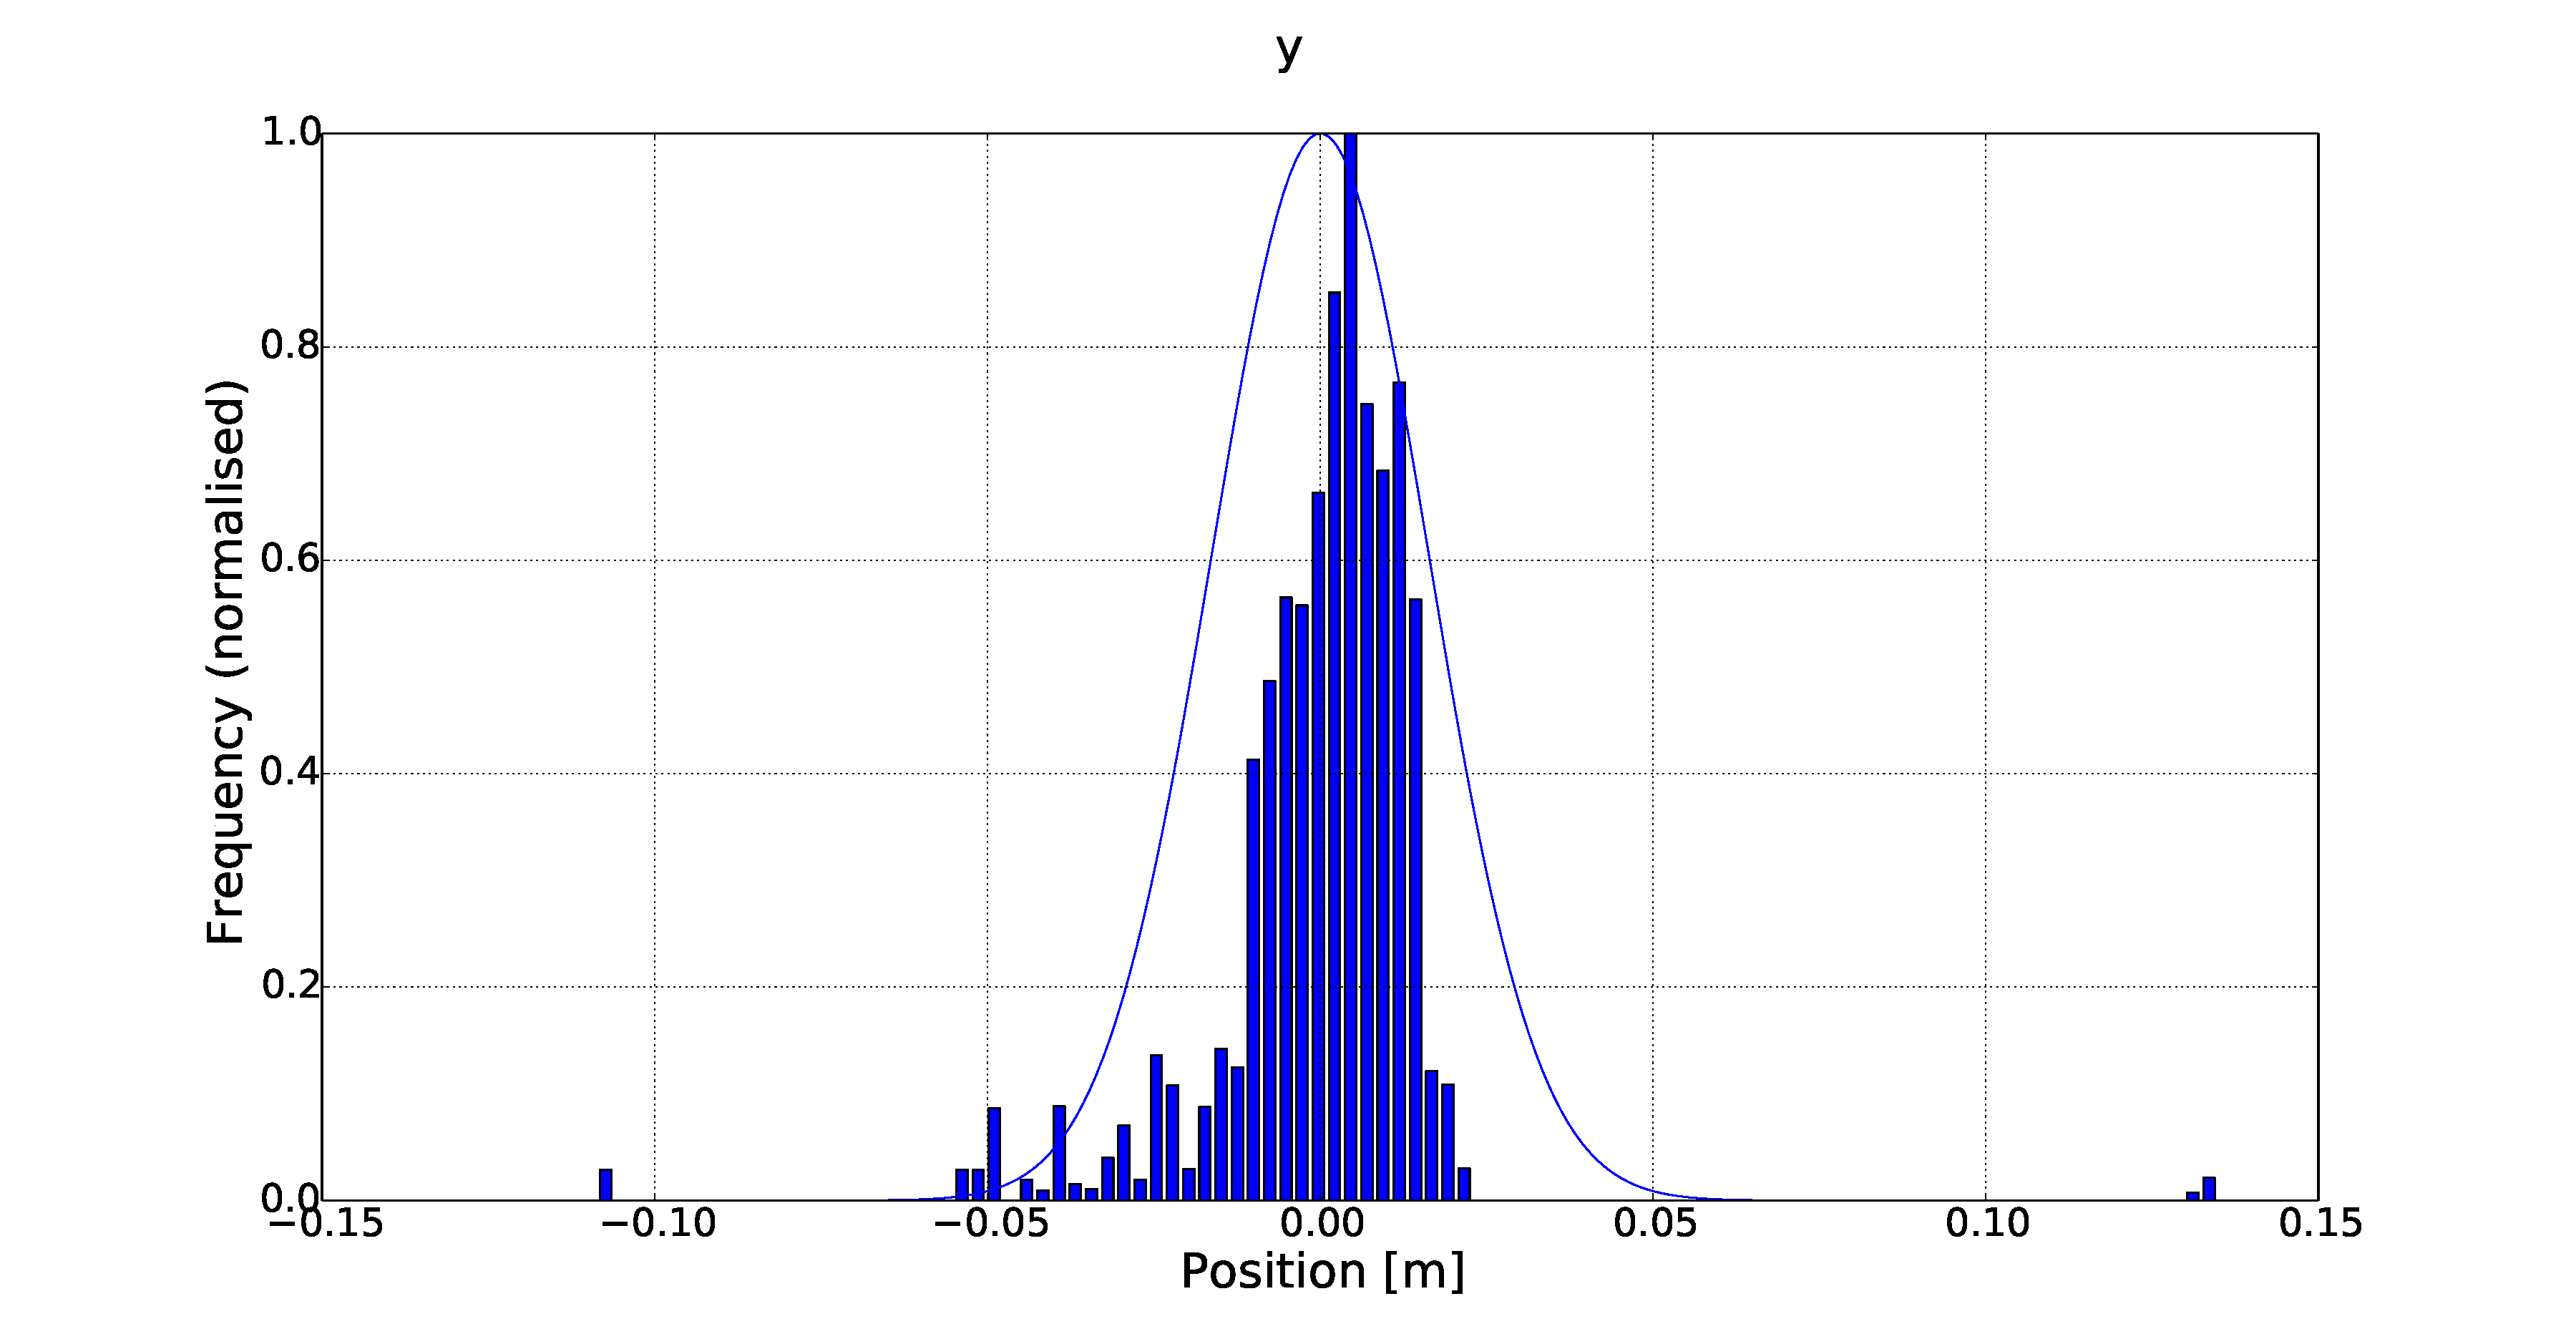
\includegraphics[clip, trim = 120 0 120 0, width=\textwidth]{figures/chapter3/norm_y}
     \caption{$\mu = \SI{0.207}{\mm}$, $\sigma = \SI{12.6}{\mm}$.}
  \label{fig:norm-y}
  \end{subfigure}
~
  \begin{subfigure}{0.48\textwidth}
     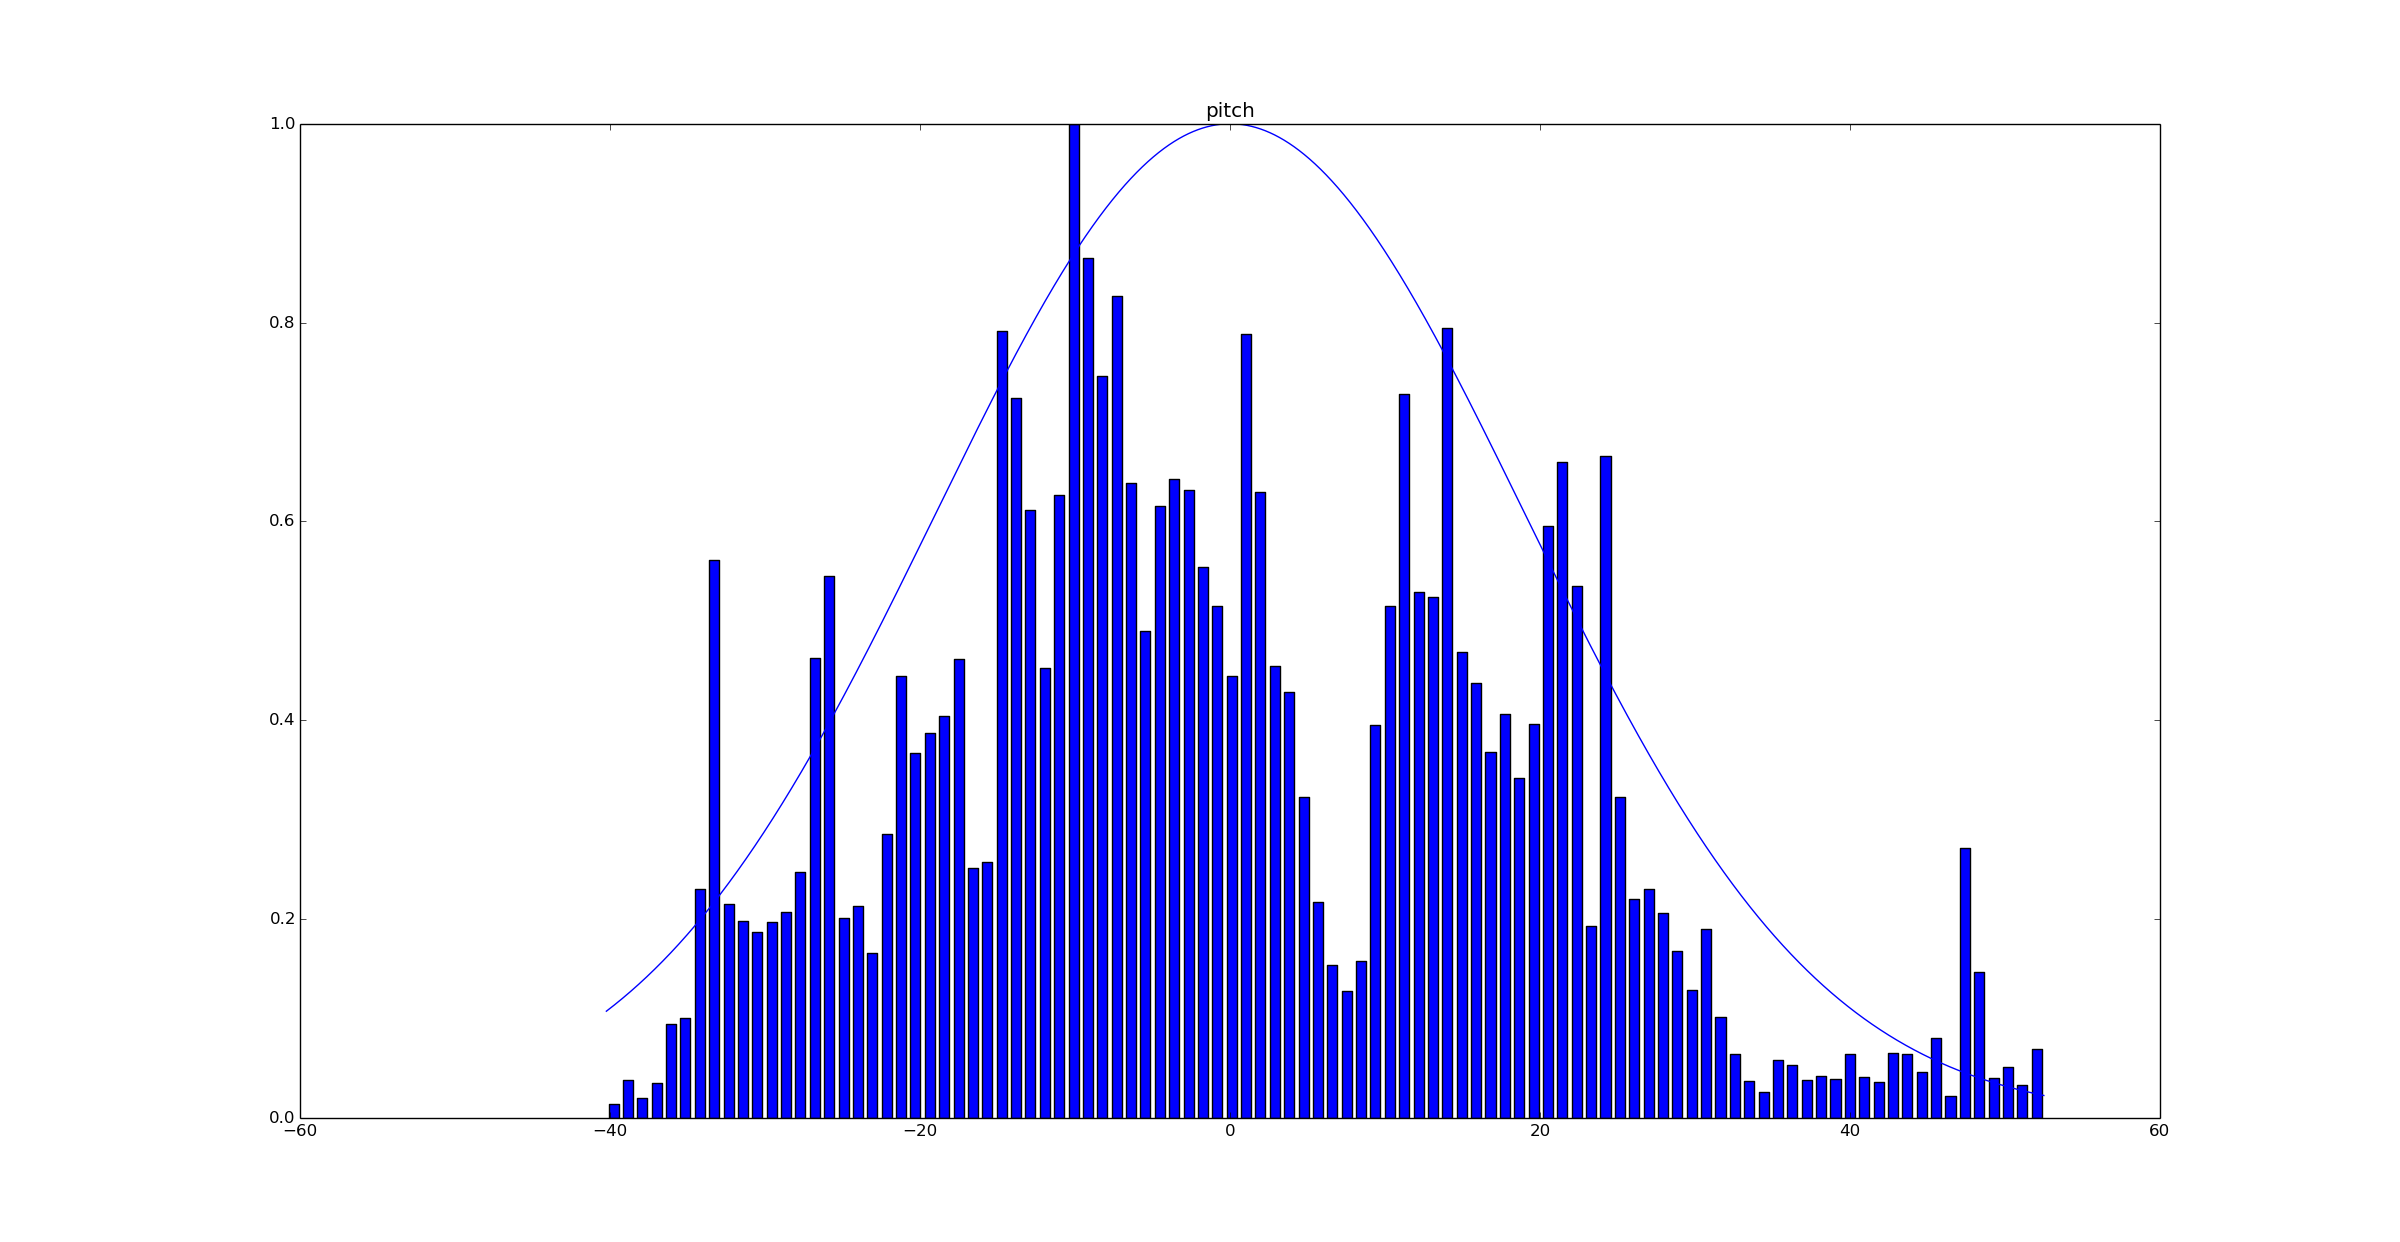
\includegraphics[clip, trim = 120 0 120 0, width=\textwidth]{figures/chapter3/norm_pitch}
     \caption{$\mu = \ang{0.914}$, $\sigma = \ang{5.99}$.}
  \label{fig:norm-pitch}
  \end{subfigure}

  \begin{subfigure}{0.48\textwidth}
     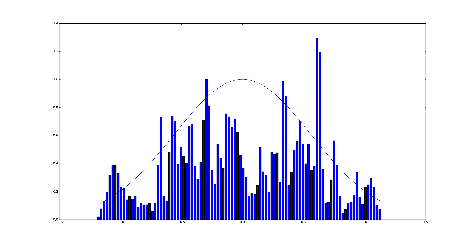
\includegraphics[clip, trim = 120 0 120 0, width=\textwidth]{figures/chapter3/norm_z}
     \caption{$\mu = \SI{-0.253}{\mm}$, $\sigma = \SI{20.8}{\mm}$.}
  \label{fig:norm-z}
  \end{subfigure}
~
\begin{subfigure}{0.48\textwidth}
     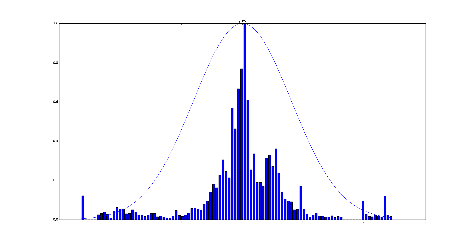
\includegraphics[clip, trim = 120 0 120 0, width=\textwidth]{figures/chapter3/norm_yaw}
     \caption{$\mu = \ang{0.320}$, $\sigma = \ang{8.11}$. }
  \label{fig:norm-yaw}
  \end{subfigure}
  \caption[Frequency histograms of the error data in each dimension.]{Frequency histograms of the error data in each dimension. Each dimension's mean value ($\mu$) and standard deviation ($\sigma$) is given in the captions. }
  \label{fig:err-norm}
\end{figure*}

From Figure~\ref{fig:err-norm} it can be seen that all the plots are roughly centred around zero and are very nearly normally distributed. The $x$ dimension displays the largest standard deviation of $\SI{32.2}{\mm}$ followed by the $z$ dimension. This implies that the $x$ dimension's estimates are the least accurate. However, upon closer inspection of Figure~\ref{fig:chap3-err-norm-x}, it can be argued that the $x$ dimension's error is uniformly distributed and not normally distributed like the other dimensions are. This would make the standard deviation an invalid measure of error. The standard deviations of the other dimensions are within the range that was expected of the system. 

In all, the frequency histogram and normal distribution plots of the errors in Figure~\ref{fig:err-norm} show that the assumption made in Equation~\ref{eq:chap3-eq2-offset} (that the errors are distributed around zero) is indeed a valid one. Furthermore, with the exception of the $x$ dimension, the error data looks to be roughly normally distributed allowing other statistical tools to be used on the data set. 

\subsection{Optimum Focal Lengths and Offset}

As a result of the focal length and offset optimisation procedure, the optimal focal lengths, $\hat{f}_x$ and $\hat{f}_y$, were found to be 694 and 704 respectively after 15 iterations of the algorithm. This is approximately the 700 which was determined by the calibration toolbox. Note that these units are given in camera pixel units and not millimetres. The optimal offset, $\bar{\bm{P}}$, was found to be 

\begin{equation}
  \label{eq:chap3-offset-value}
  \bar{\bm{P}} = 
  \begin{bmatrix}
    \SI{283.8}{\mm} & \SI{56.16}{\mm} & \SI{-57.44}{\mm} & \ang{179.8} & \ang{-1.305} & \ang{-178.8}
  \end{bmatrix}^T.
\end{equation}
The values in $\bar{\bm{P}}$ contain any constant error bias as well as marker placement errors that may have been introduced to the Vicon test during the measurement process. The large offsets of $\pm\ang{180}$ in the $roll$ and $yaw$ dimensions can be explained by the differing axis orientations of the CVS camera and Vicon systems, where the axes needed to be rotated to coincide with one another. This indicates that the offset was correctly calculated and was working as expected. The relatively large offset in the $x$ dimension was surprising initially, since this indicated that there was a large constant level of error bias introduced to the $x$ dimension's measurements. However, this would make sense if the CVS's camera was placed approximately $\SI{280}{\mm}$ from the Vicon's axis centre. It turns out this was indeed the case. 

All of the above produce an error two-norm of approximately 1.01 (normalised), compared to the original 1.15 (normalised), showing an overall reduction in the error vector magnitude. The optimal focal lengths are fairly similar to the focal lengths given by OpenCV's calibration procedure, which is within the range that was expected. Figures~\ref{fig:estimate-x} to~\ref{fig:estimate-yaw} show the results of the Vicon measurements compared to the original and improved CVS measurements in all six dimensions.

\begin{figure}
  \centering
  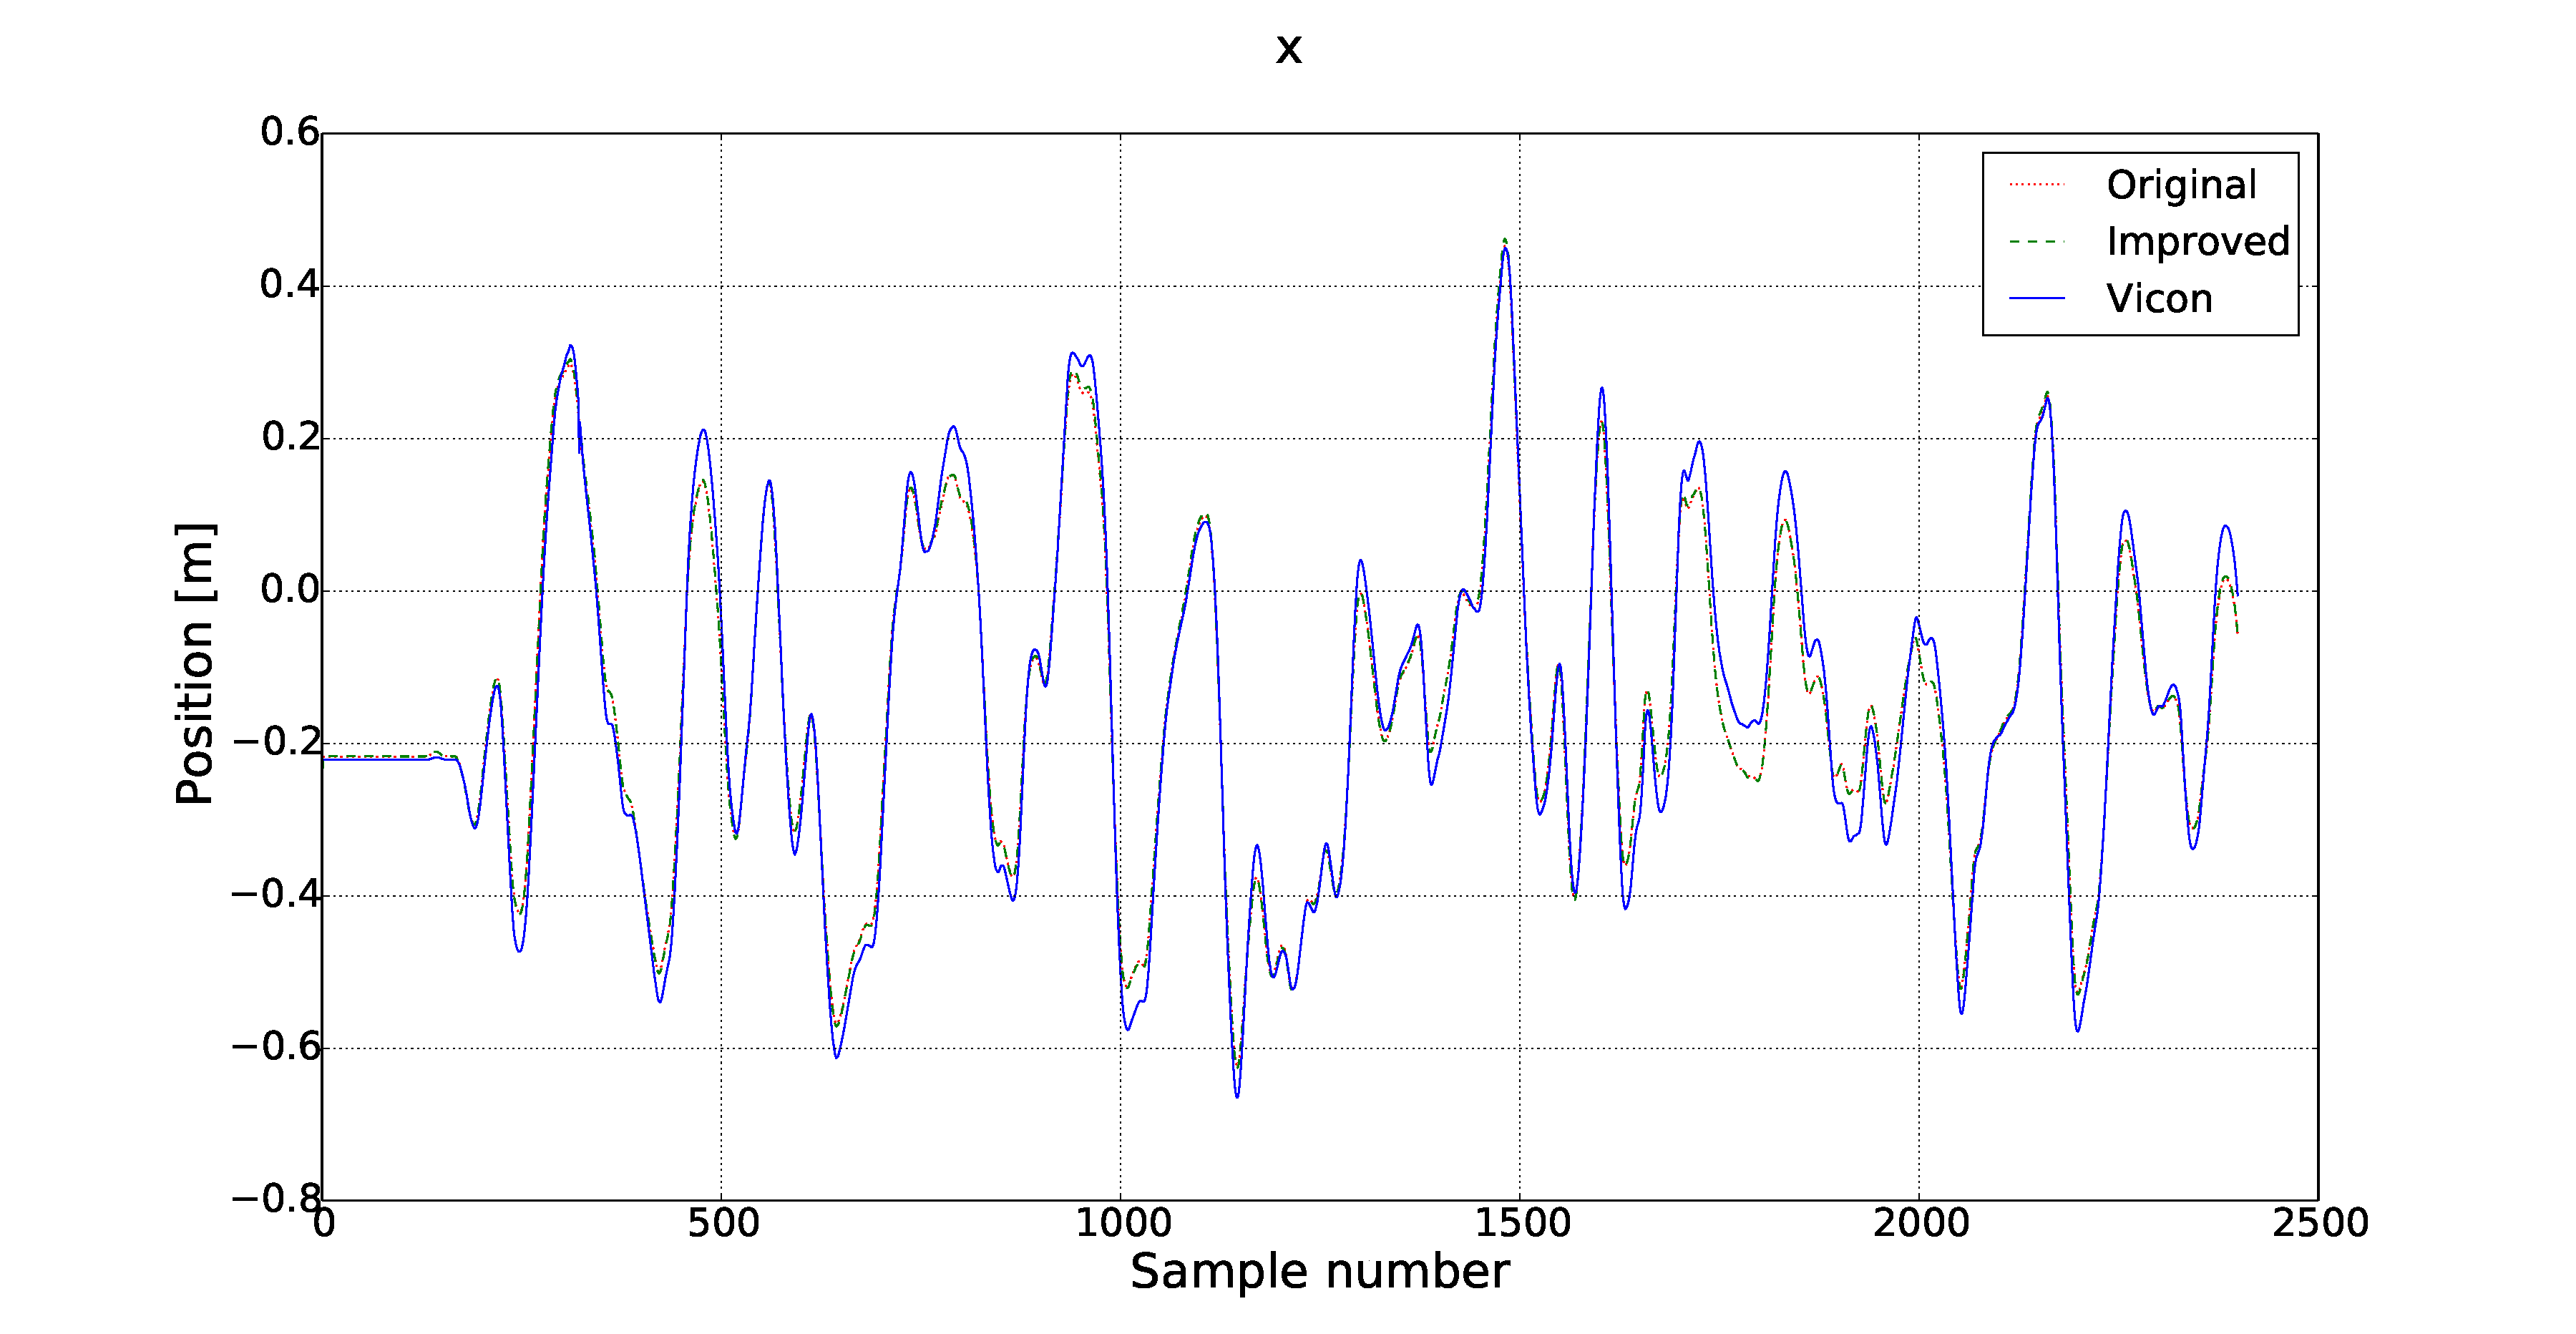
\includegraphics[clip, trim = 100 0 140 0, width=\textwidth]{figures/chapter3/x}
  \caption{Plot comparing the Vicon, original and improved CVS measurements in the $x$ dimension.}
  \label{fig:estimate-x}
\end{figure}
\begin{figure}
  \centering
  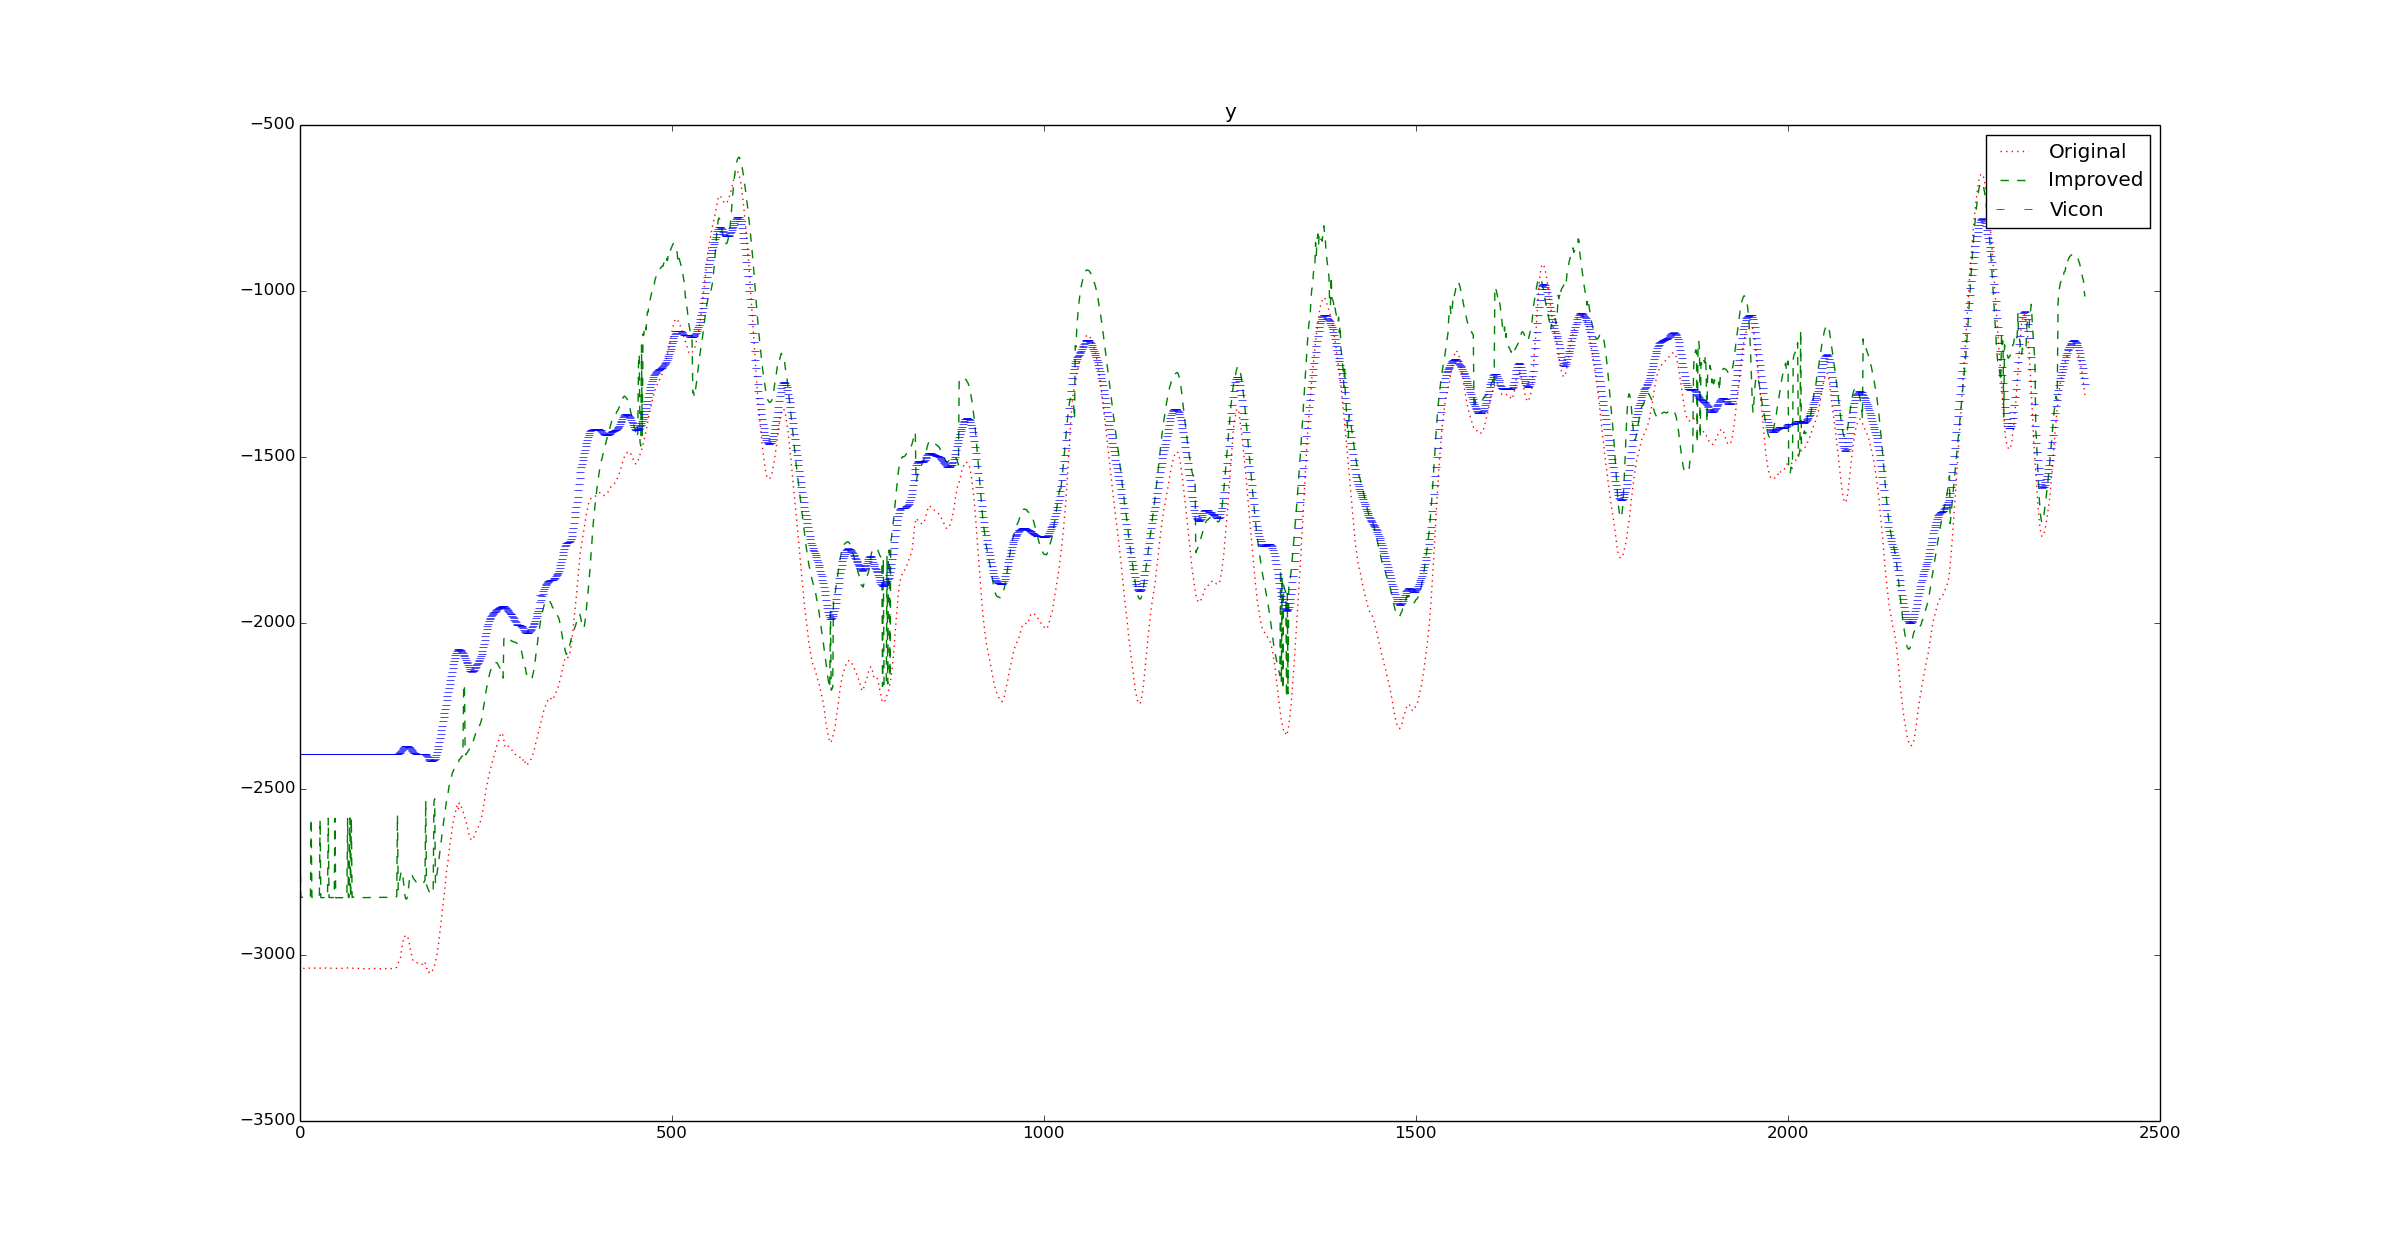
\includegraphics[clip, trim = 100 0 140 0, width=\textwidth]{figures/chapter3/y}
  \caption{Plot comparing the Vicon, original and improved CVS measurements in the $y$ dimension.}
\end{figure}
\begin{figure}
  \centering
  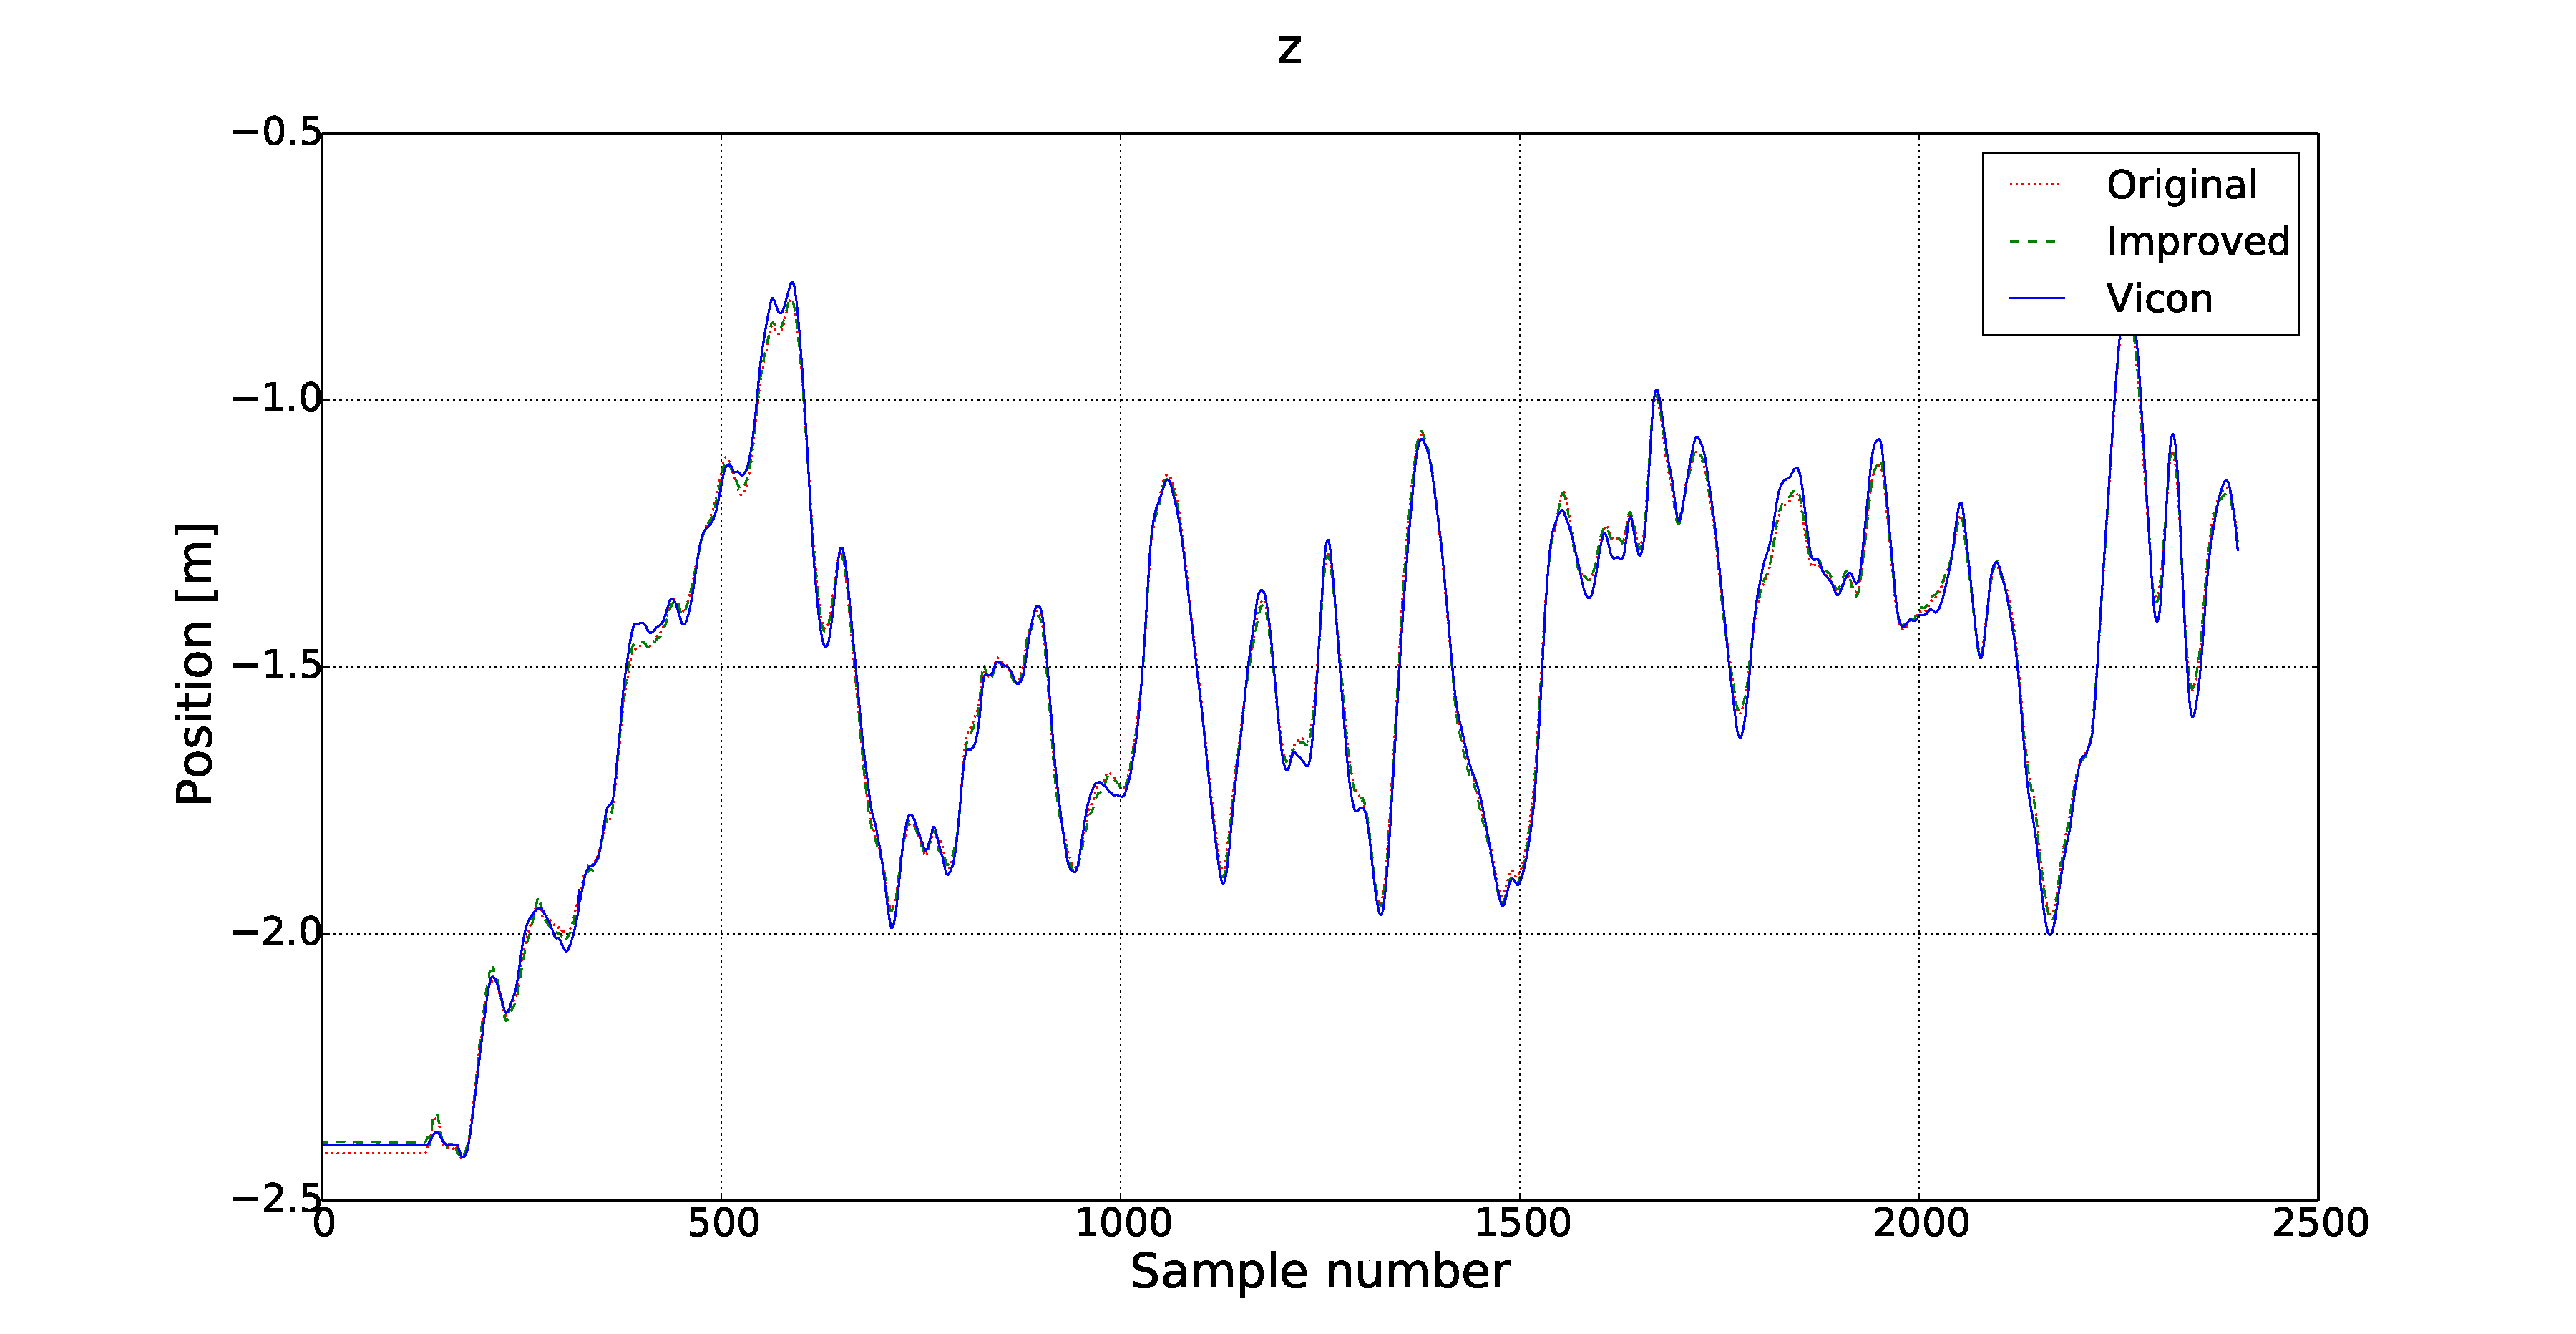
\includegraphics[clip, trim = 100 0 140 0, width=\textwidth]{figures/chapter3/z}
  \caption{Plot comparing the Vicon, original and improved CVS measurements in the $z$ dimension.}
\end{figure}
\begin{figure}
  \centering
  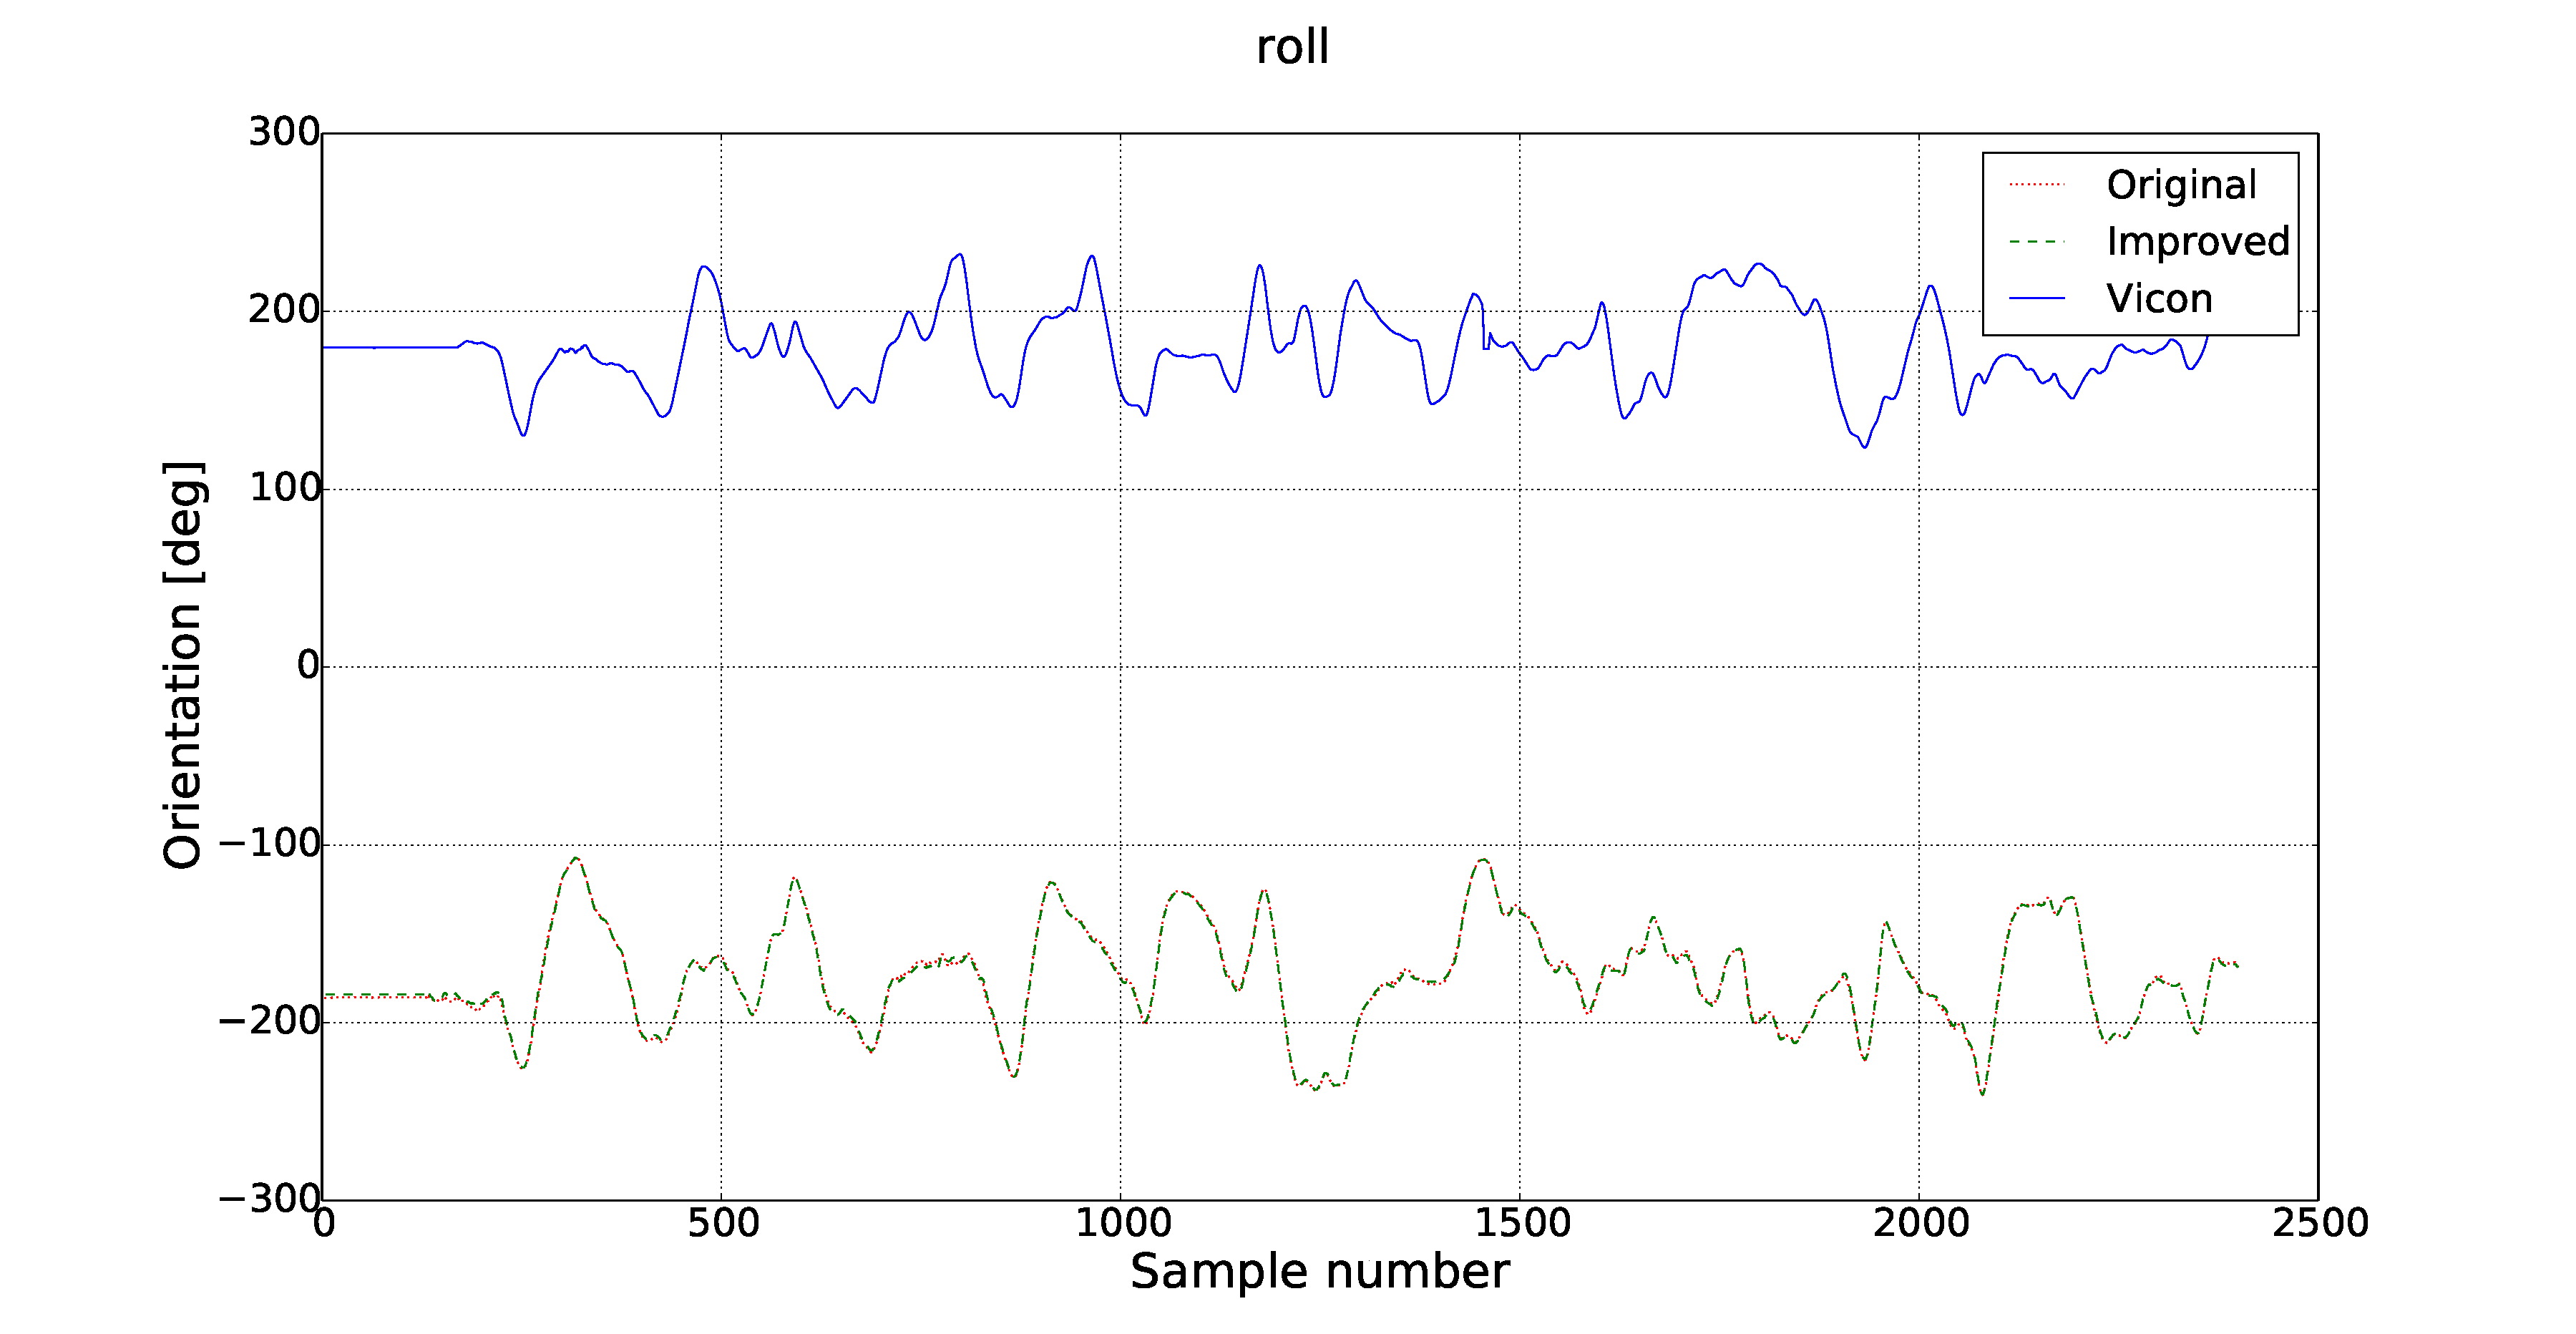
\includegraphics[clip, trim = 100 0 140 0, width=\textwidth]{figures/chapter3/roll}
  \caption{Plot comparing the Vicon, original and improved CVS measurements in the $roll$ dimension.}
\end{figure}
\begin{figure}
  \centering
  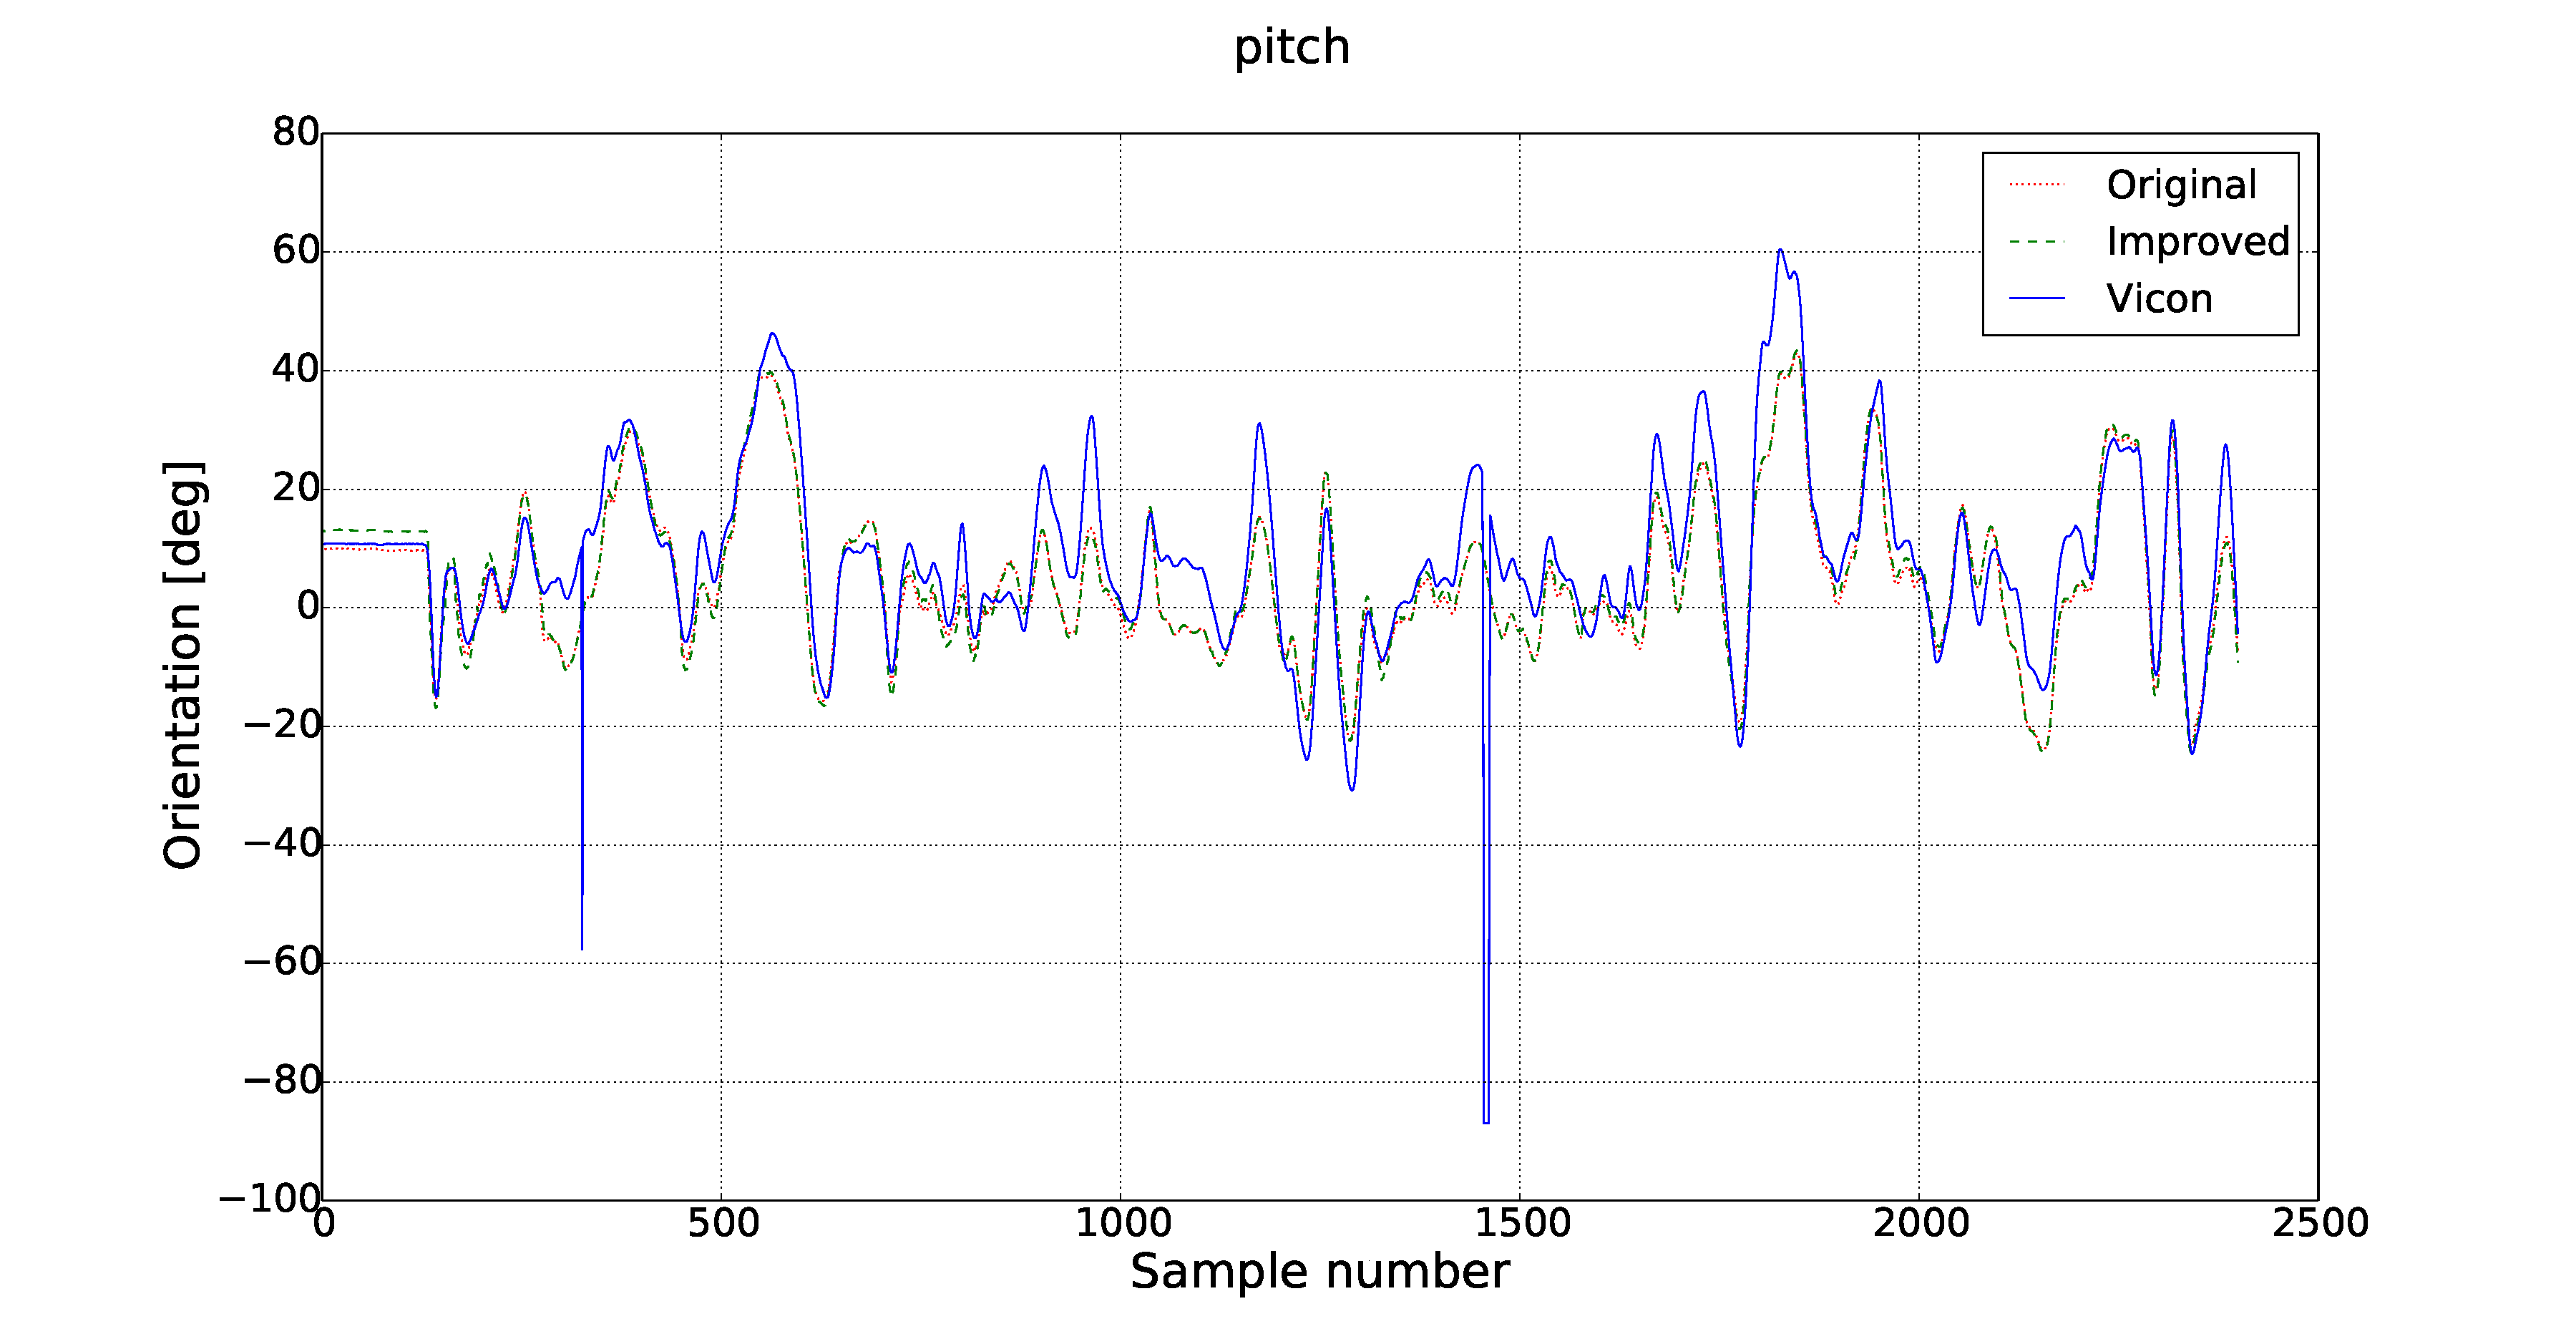
\includegraphics[clip, trim = 100 0 140 0, width=\textwidth]{figures/chapter3/pitch}
  \caption{Plot comparing the Vicon, original and improved CVS measurements in the $pitch$ dimension.}
\end{figure}
\begin{figure}
  \centering
  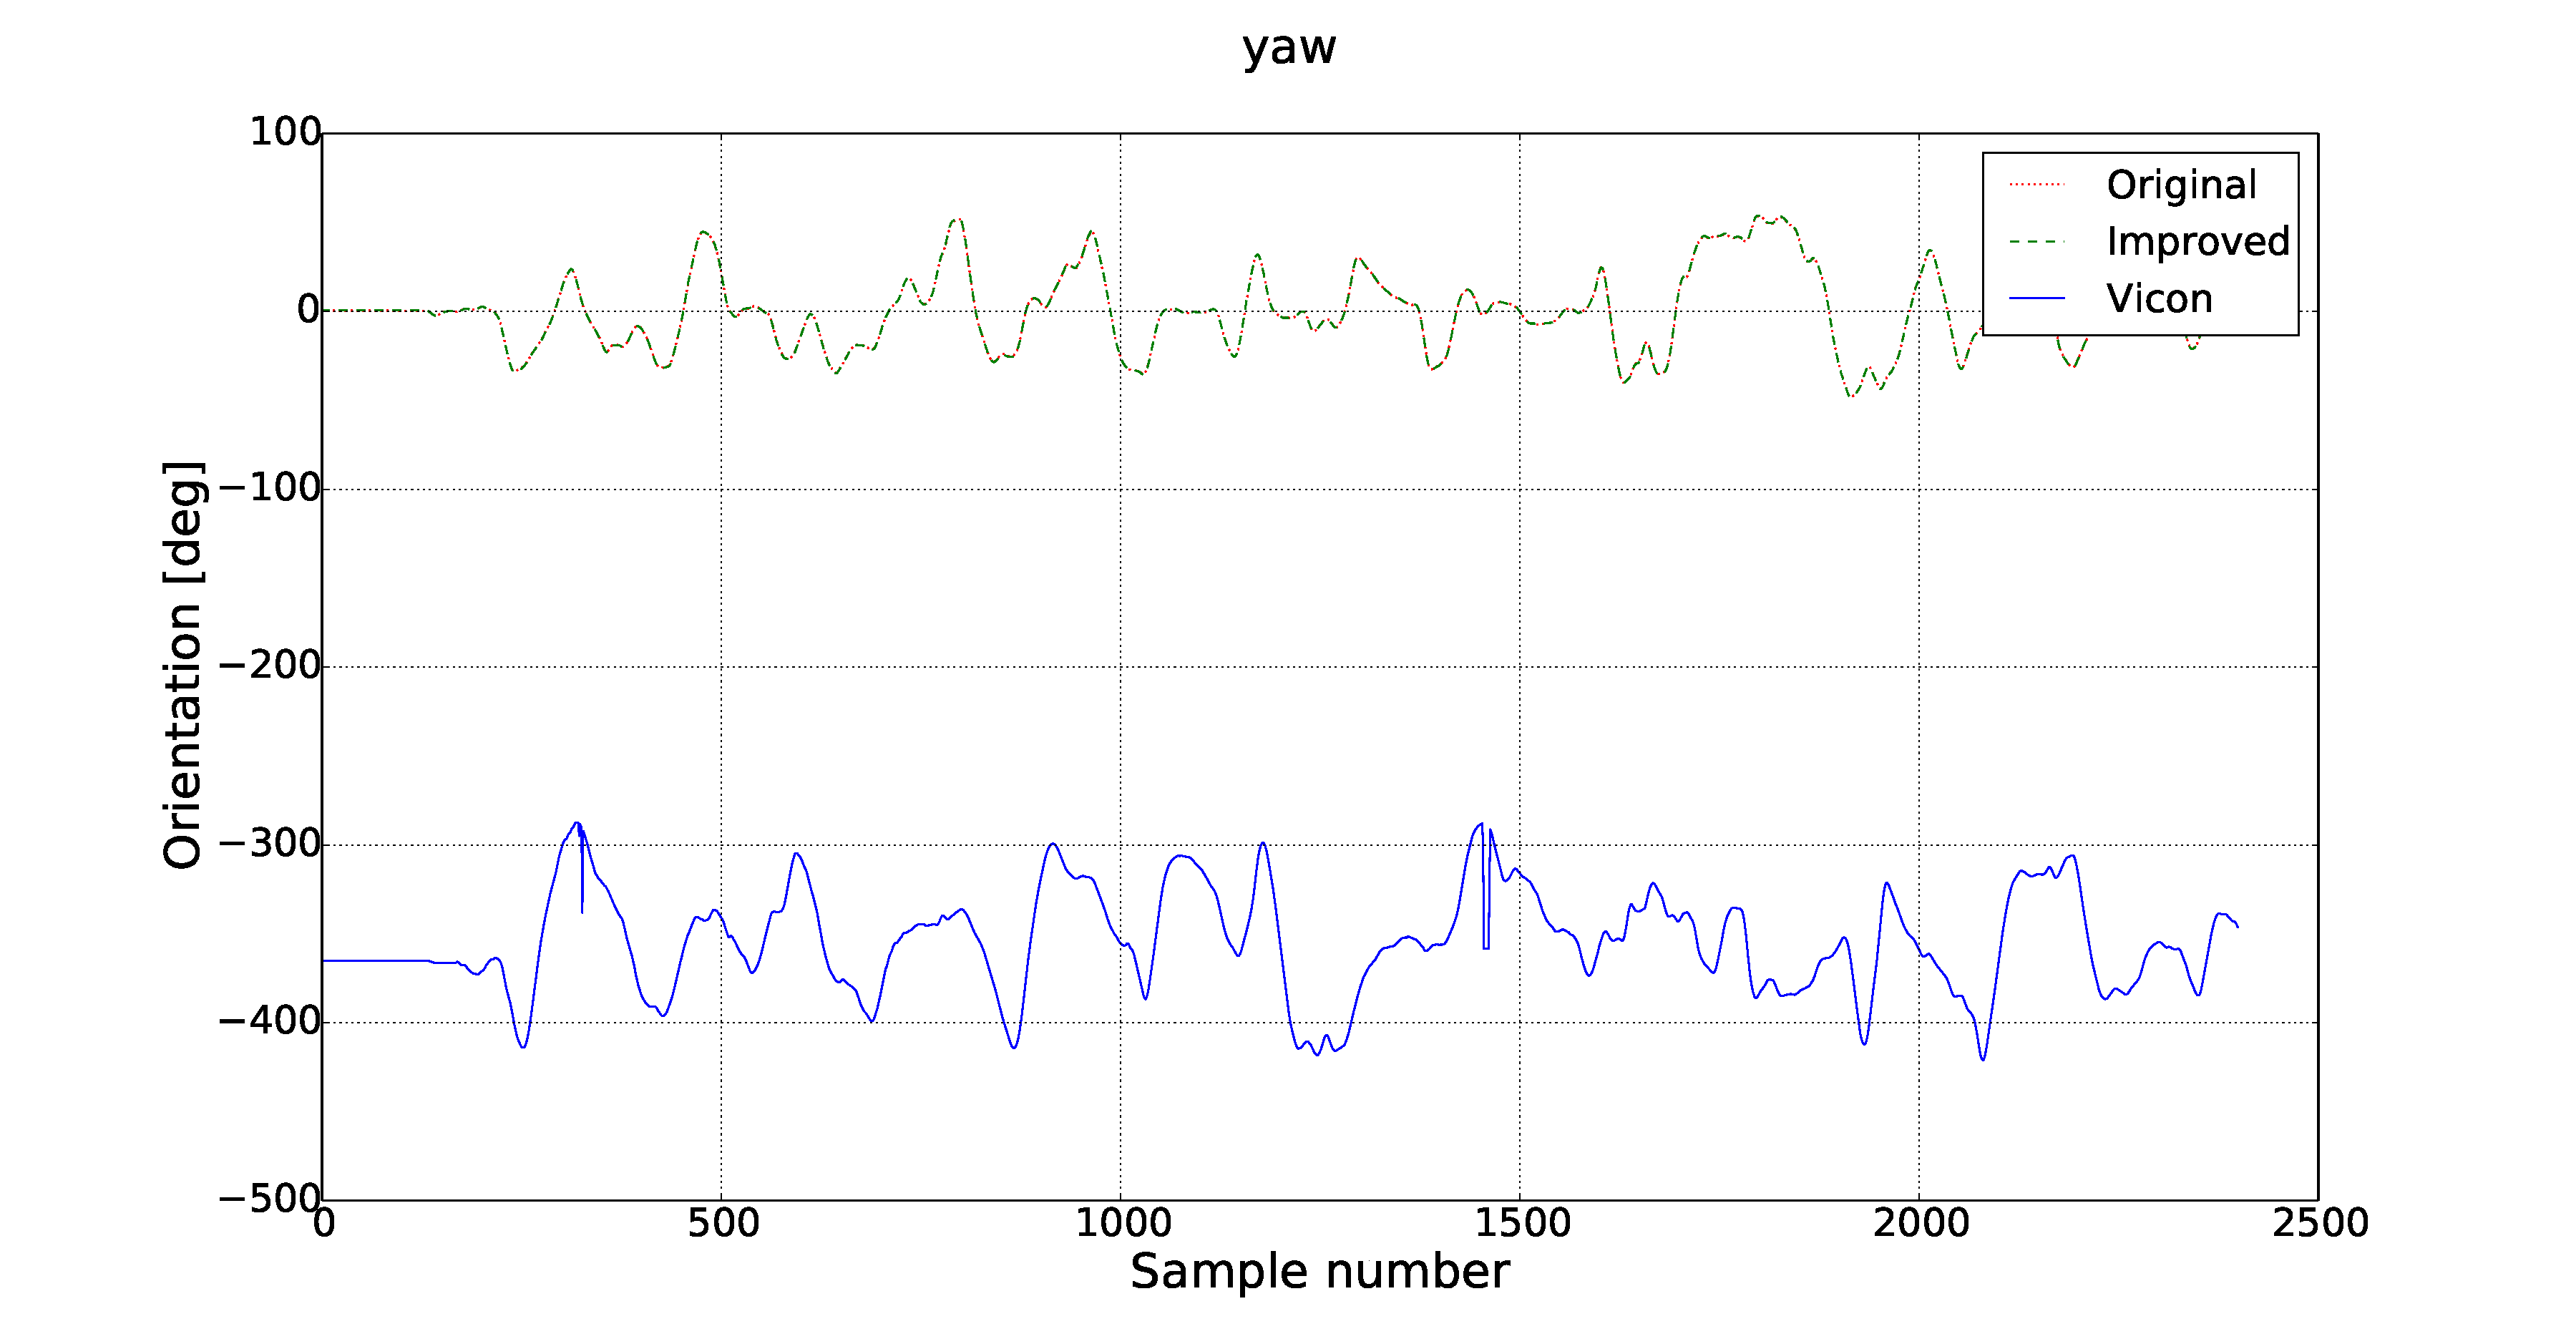
\includegraphics[clip, trim = 100 0 140 0, width=\textwidth]{figures/chapter3/yaw}
  \caption{Plot comparing the Vicon, original and improved CVS measurements in the $yaw$ dimension.}
  \label{fig:estimate-yaw}
\end{figure}

It can be seen that there is some improvement in all of the dimensions. However, in some cases the improvement in one section of the data set is negated by worse estimates in another. This can be attributed to the optimisation process, where an improvement at timeframe $t_i$ in the $x$ dimension, for example, may lead to a worse estimate at time $t_i$ in the $roll$ dimension. However, as the reduction in the two-norm magnitude of the error proves, there is an overall reduction in the error with the optimised data set. It can therefore be concluded that the optimisation procedure did indeed function as expected, producing a focal length combination which led to a more accurate pose estimate from the CVS. 

\subsection{Computer Vision System Accuracy}

Determining the accuracy of a multi-dimensional data model is often a complex task, but since it was found that the error $\bm{\epsilon}$ is normally distributed about zero, it is possible to use the covariance matrix to check the interdimensional variance and dependence. If the off-diagonal elements of the covariance matrix are sufficiently small relative to the diagonal elements, it can be assumed that the dimensions are strong enough independent of one another. The covariance matrix, $\Sigma$, is given by Equation~\ref{eq:covariance-matrix}. 

\setlength{\arraycolsep}{2pt}
\footnotesize
\begin{equation}
  \label{eq:covariance-matrix}
  \Sigma = 
  \begin{bmatrix}
    \bm{1.05\e{-3}}  &  2.10\e{-4}       &  8.91\e{-6}       &  4.64\e{-2}       &  4.14\e{-2}      &  2.06\e{-2}       \\
    2.10\e{-4}       &  \bm{1.60\e{-4}}  &  7.31\e{-5}       &  9.12\e{-3}       &  3.30\e{-2}      & -1.66\e{-2}       \\
    8.91\e{-4}       &  7.31\e{-5}       &  \bm{4.32\e{-4}}  & -2.39\e{-3}       &  3.25\e{-2}      & -8.08\e{-3}       \\
    4.64\e{-2}       &  9.11\e{-3}       & -2.39\e{-3}       &  \bm{-1.07\e{1}}  &  7.22\e{0}       &  1.26\e{0}        \\
    4.14\e{-2}       &  3.30\e{-2}       &  3.34\e{-2}       &  7.22\e{0}        &  \bm{3.59\e{1}}  &  2.91\e{0}        \\
    2.06\e{-2}       &  1.66\e{-2}       & -8.08\e{-3}       &  1.26\e{0}        &  2.91\e{0}       &  \bm{6.59\e{1}}   \\
  \end{bmatrix}
  \end{equation}
\normalsize

The matrix $\Sigma$ displays large off-diagonal elements, indicating that there is strong interdimensionally dependant relationships. This dependence is further demonstrated when examining the change in a dimension's error with respect to the other dimensions, demonstrated by the contour plots of Figure~\ref{fig:err-contour}. 

\begin{figure*}
  \centering
  \begin{subfigure}{0.48\textwidth}
    \begin{subfigure}{\textwidth}
      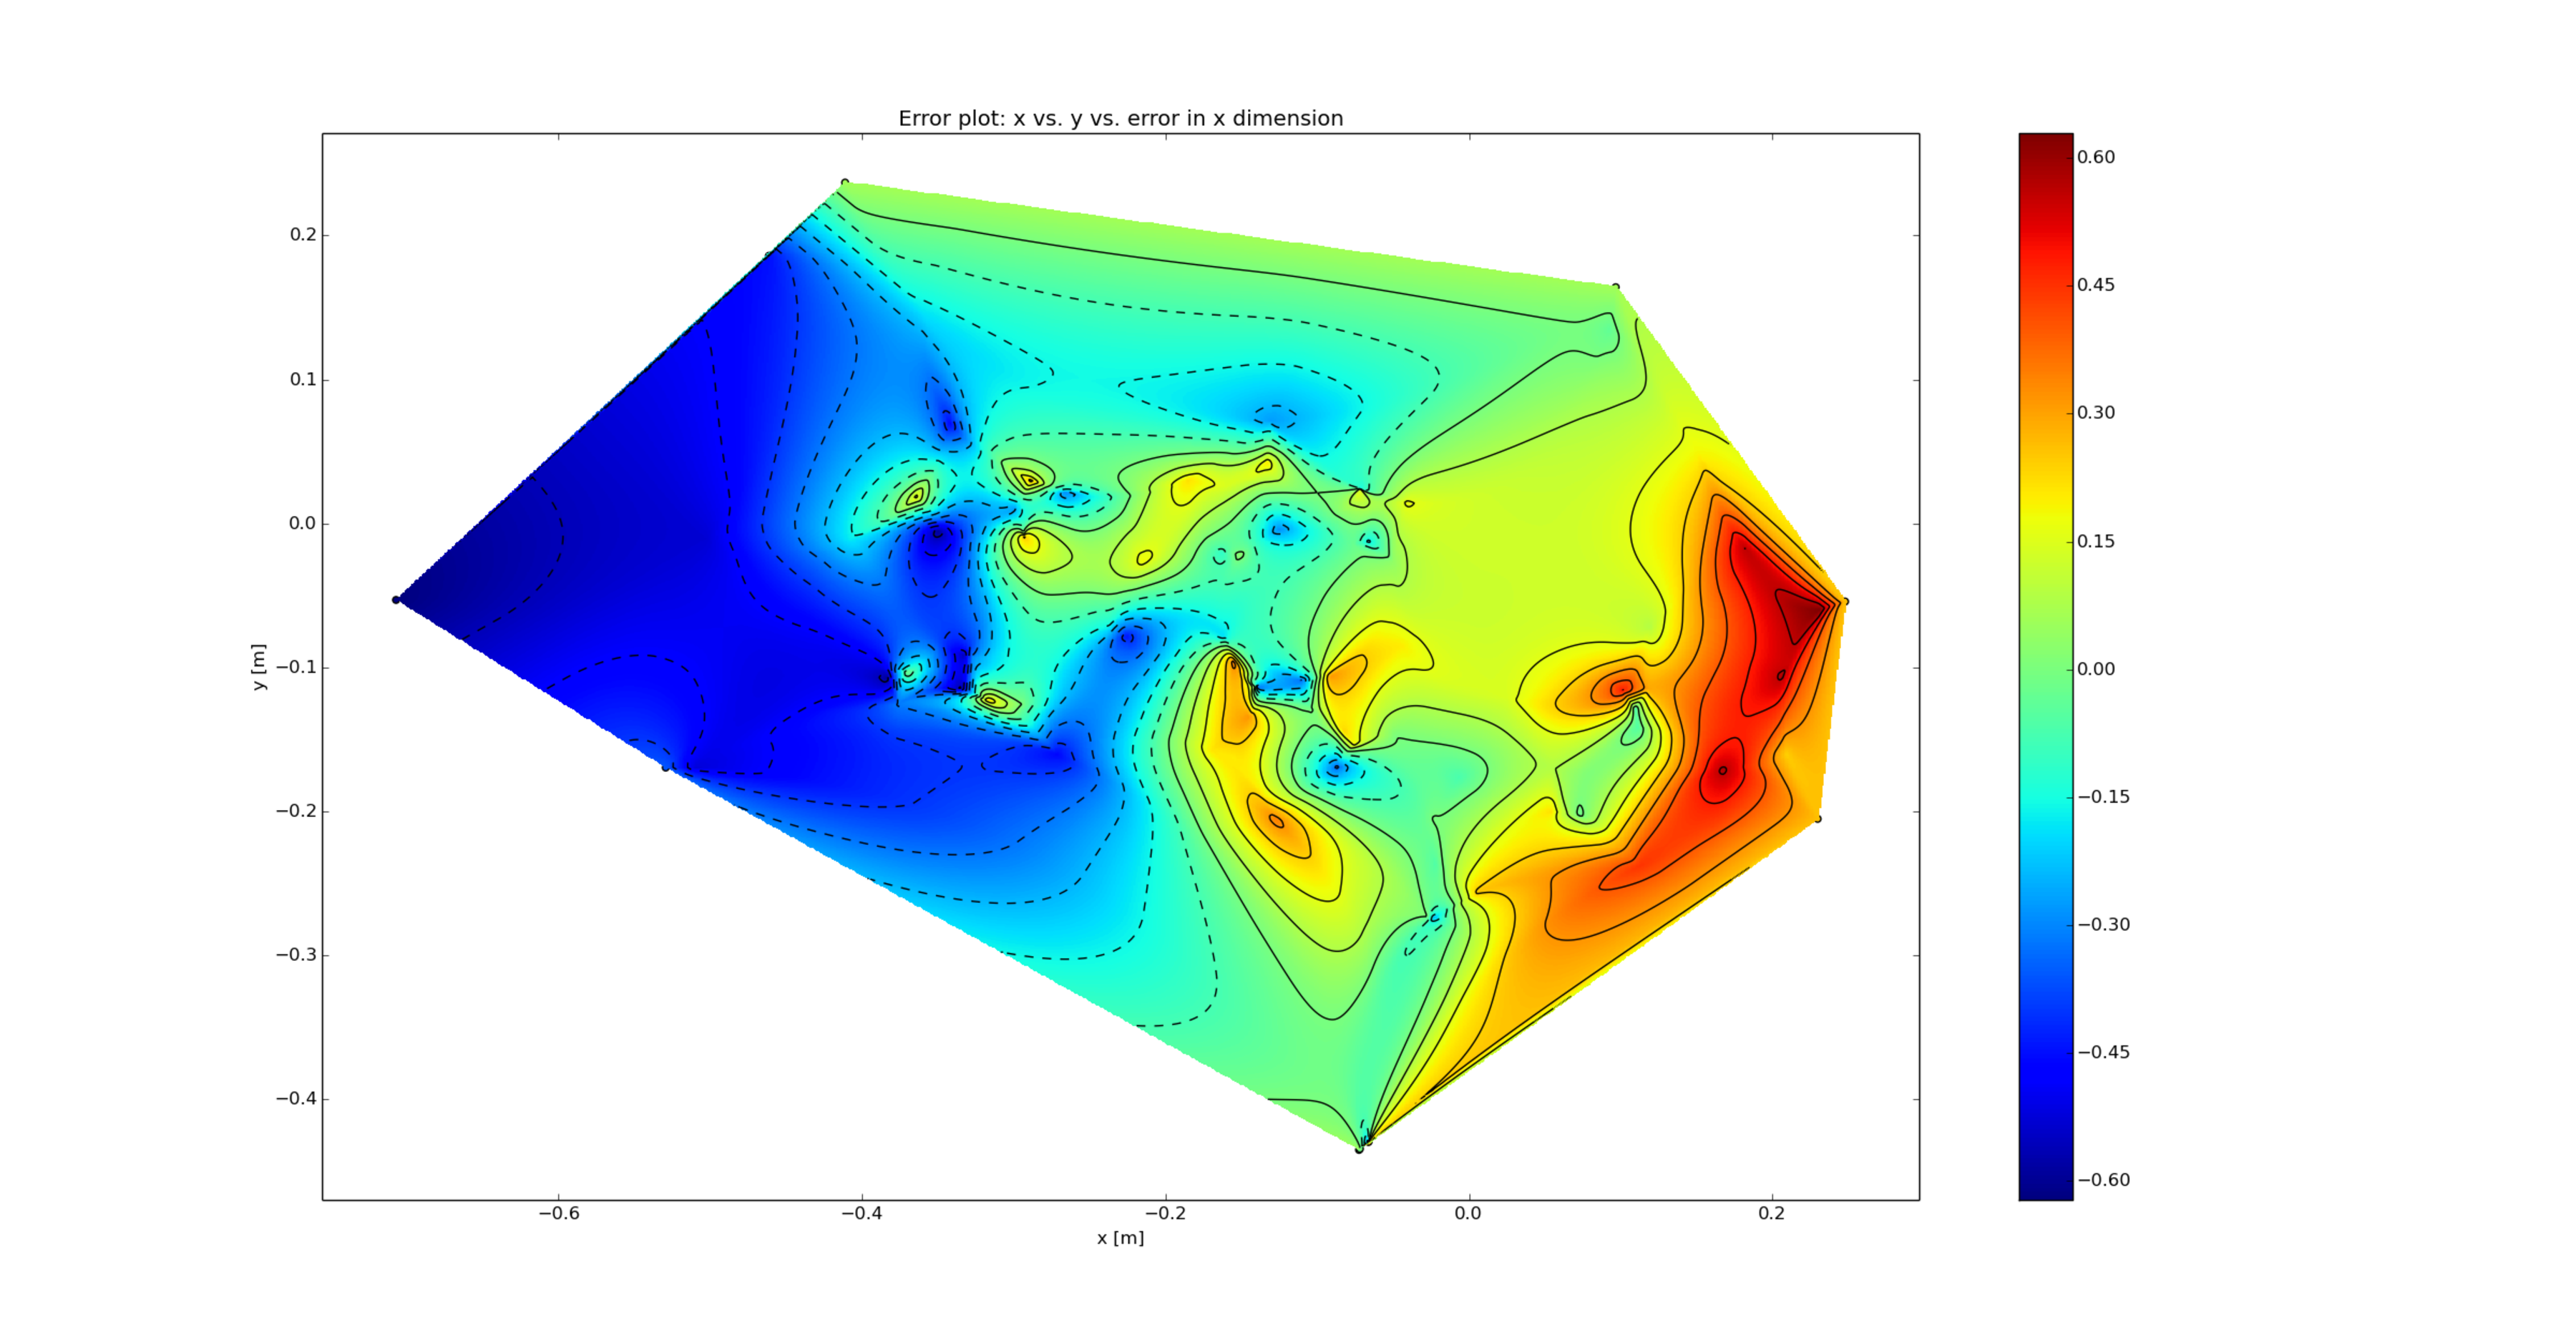
\includegraphics[clip, trim = 20 0 150 0, width=\textwidth]{figures/chapter3/contour_x}
    \end{subfigure}
    \begin{subfigure}{\textwidth}
      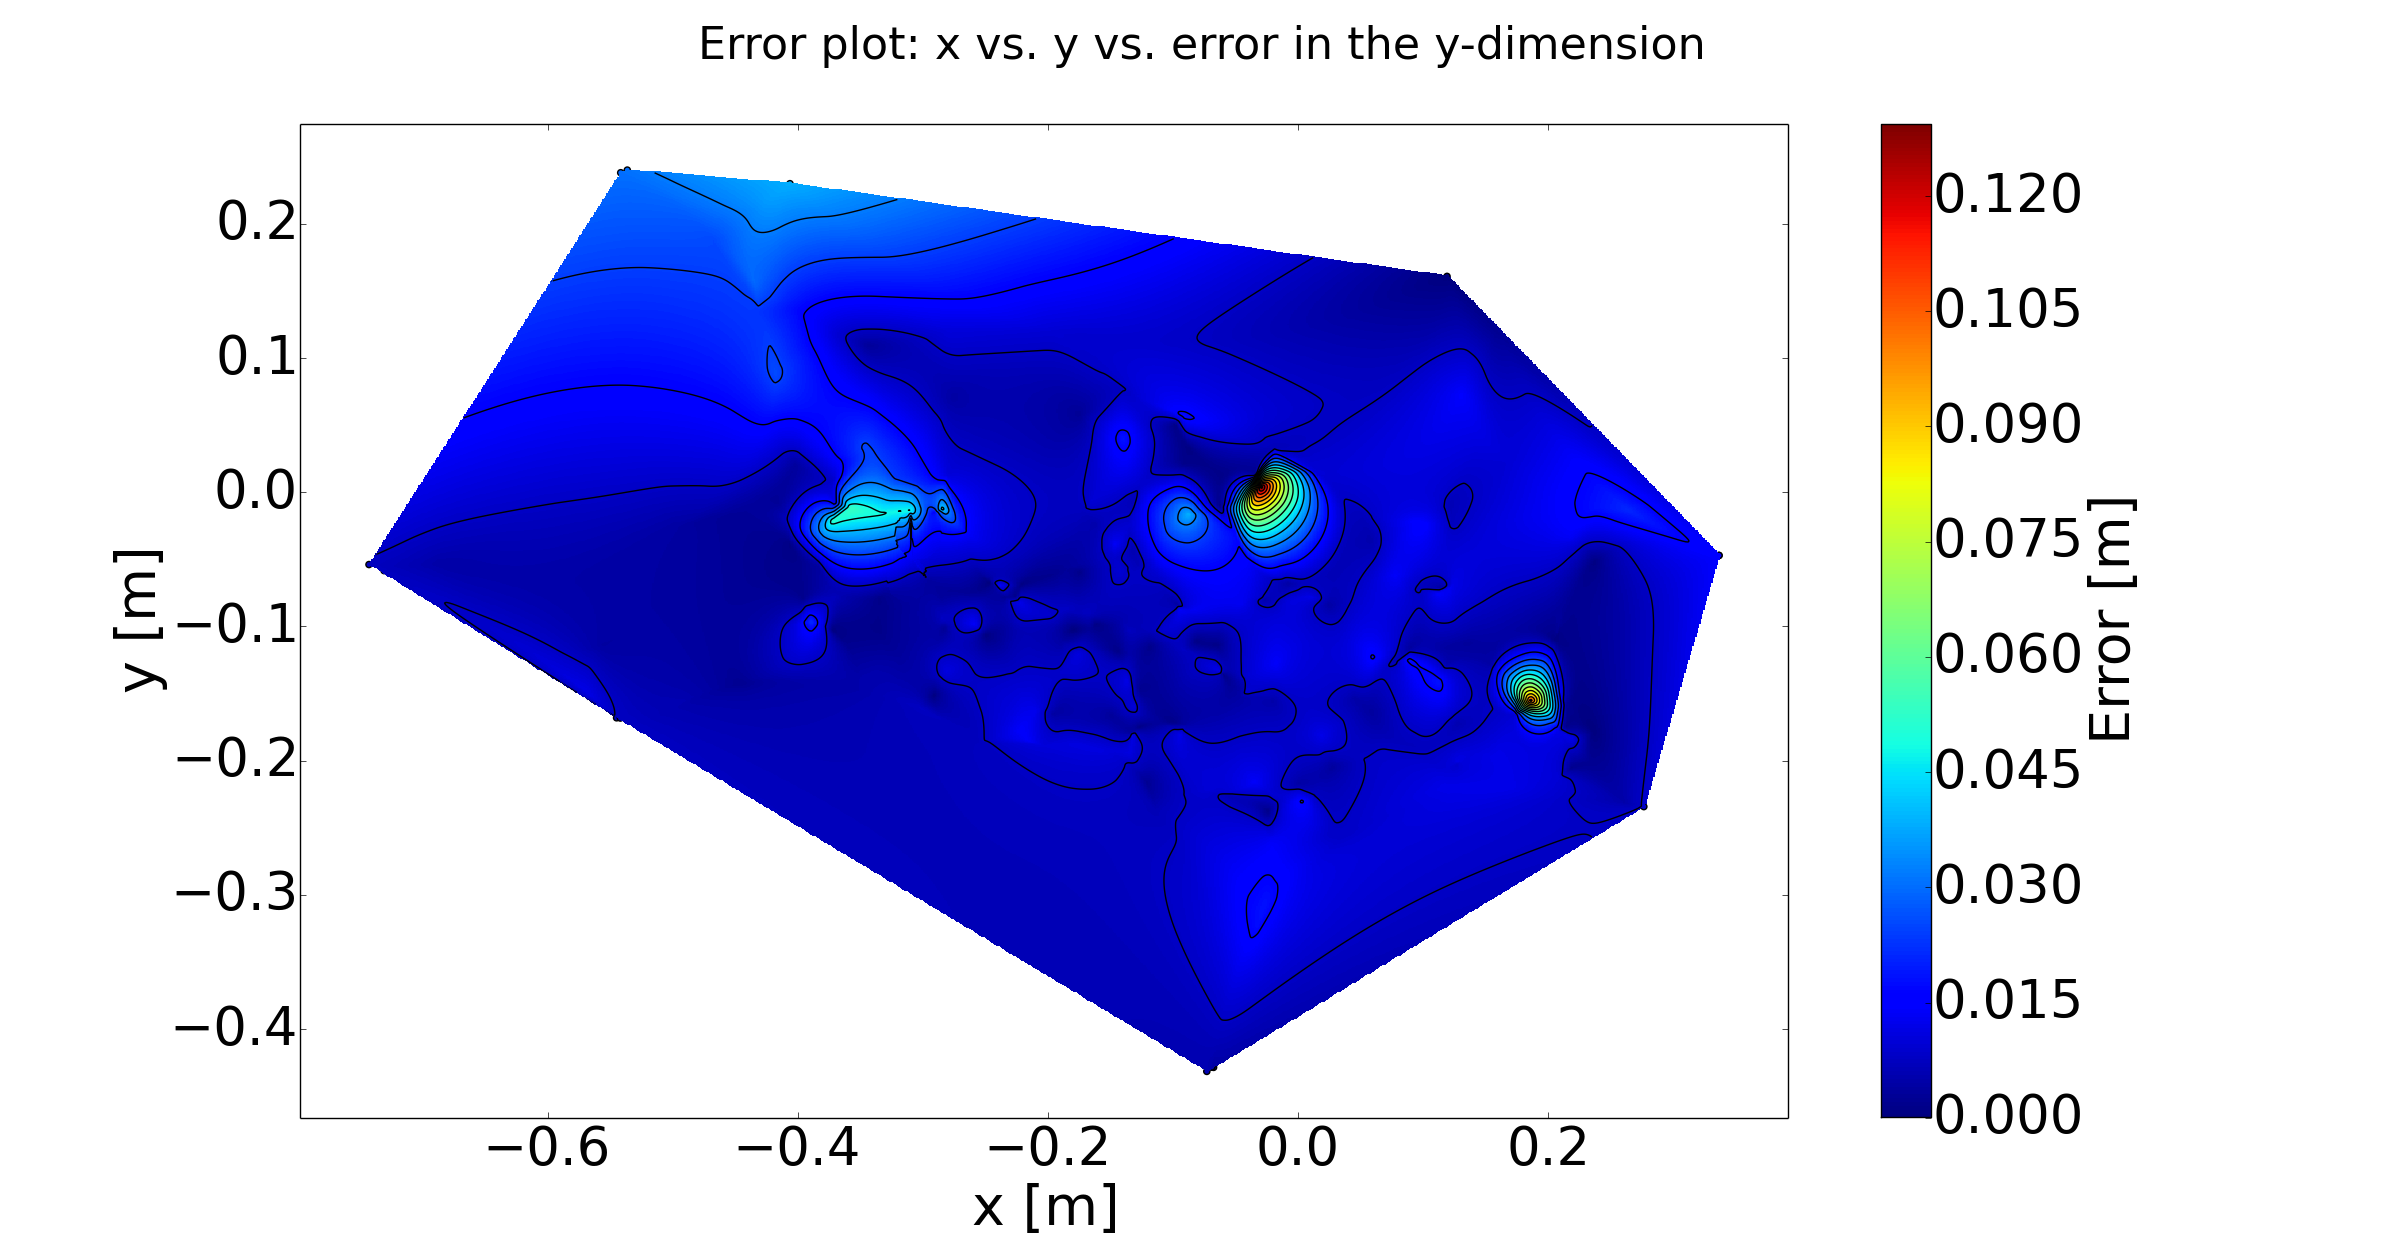
\includegraphics[clip, trim = 20 0 150 0, width=\textwidth]{figures/chapter3/contour_y}
    \end{subfigure}
    \begin{subfigure}{\textwidth}
      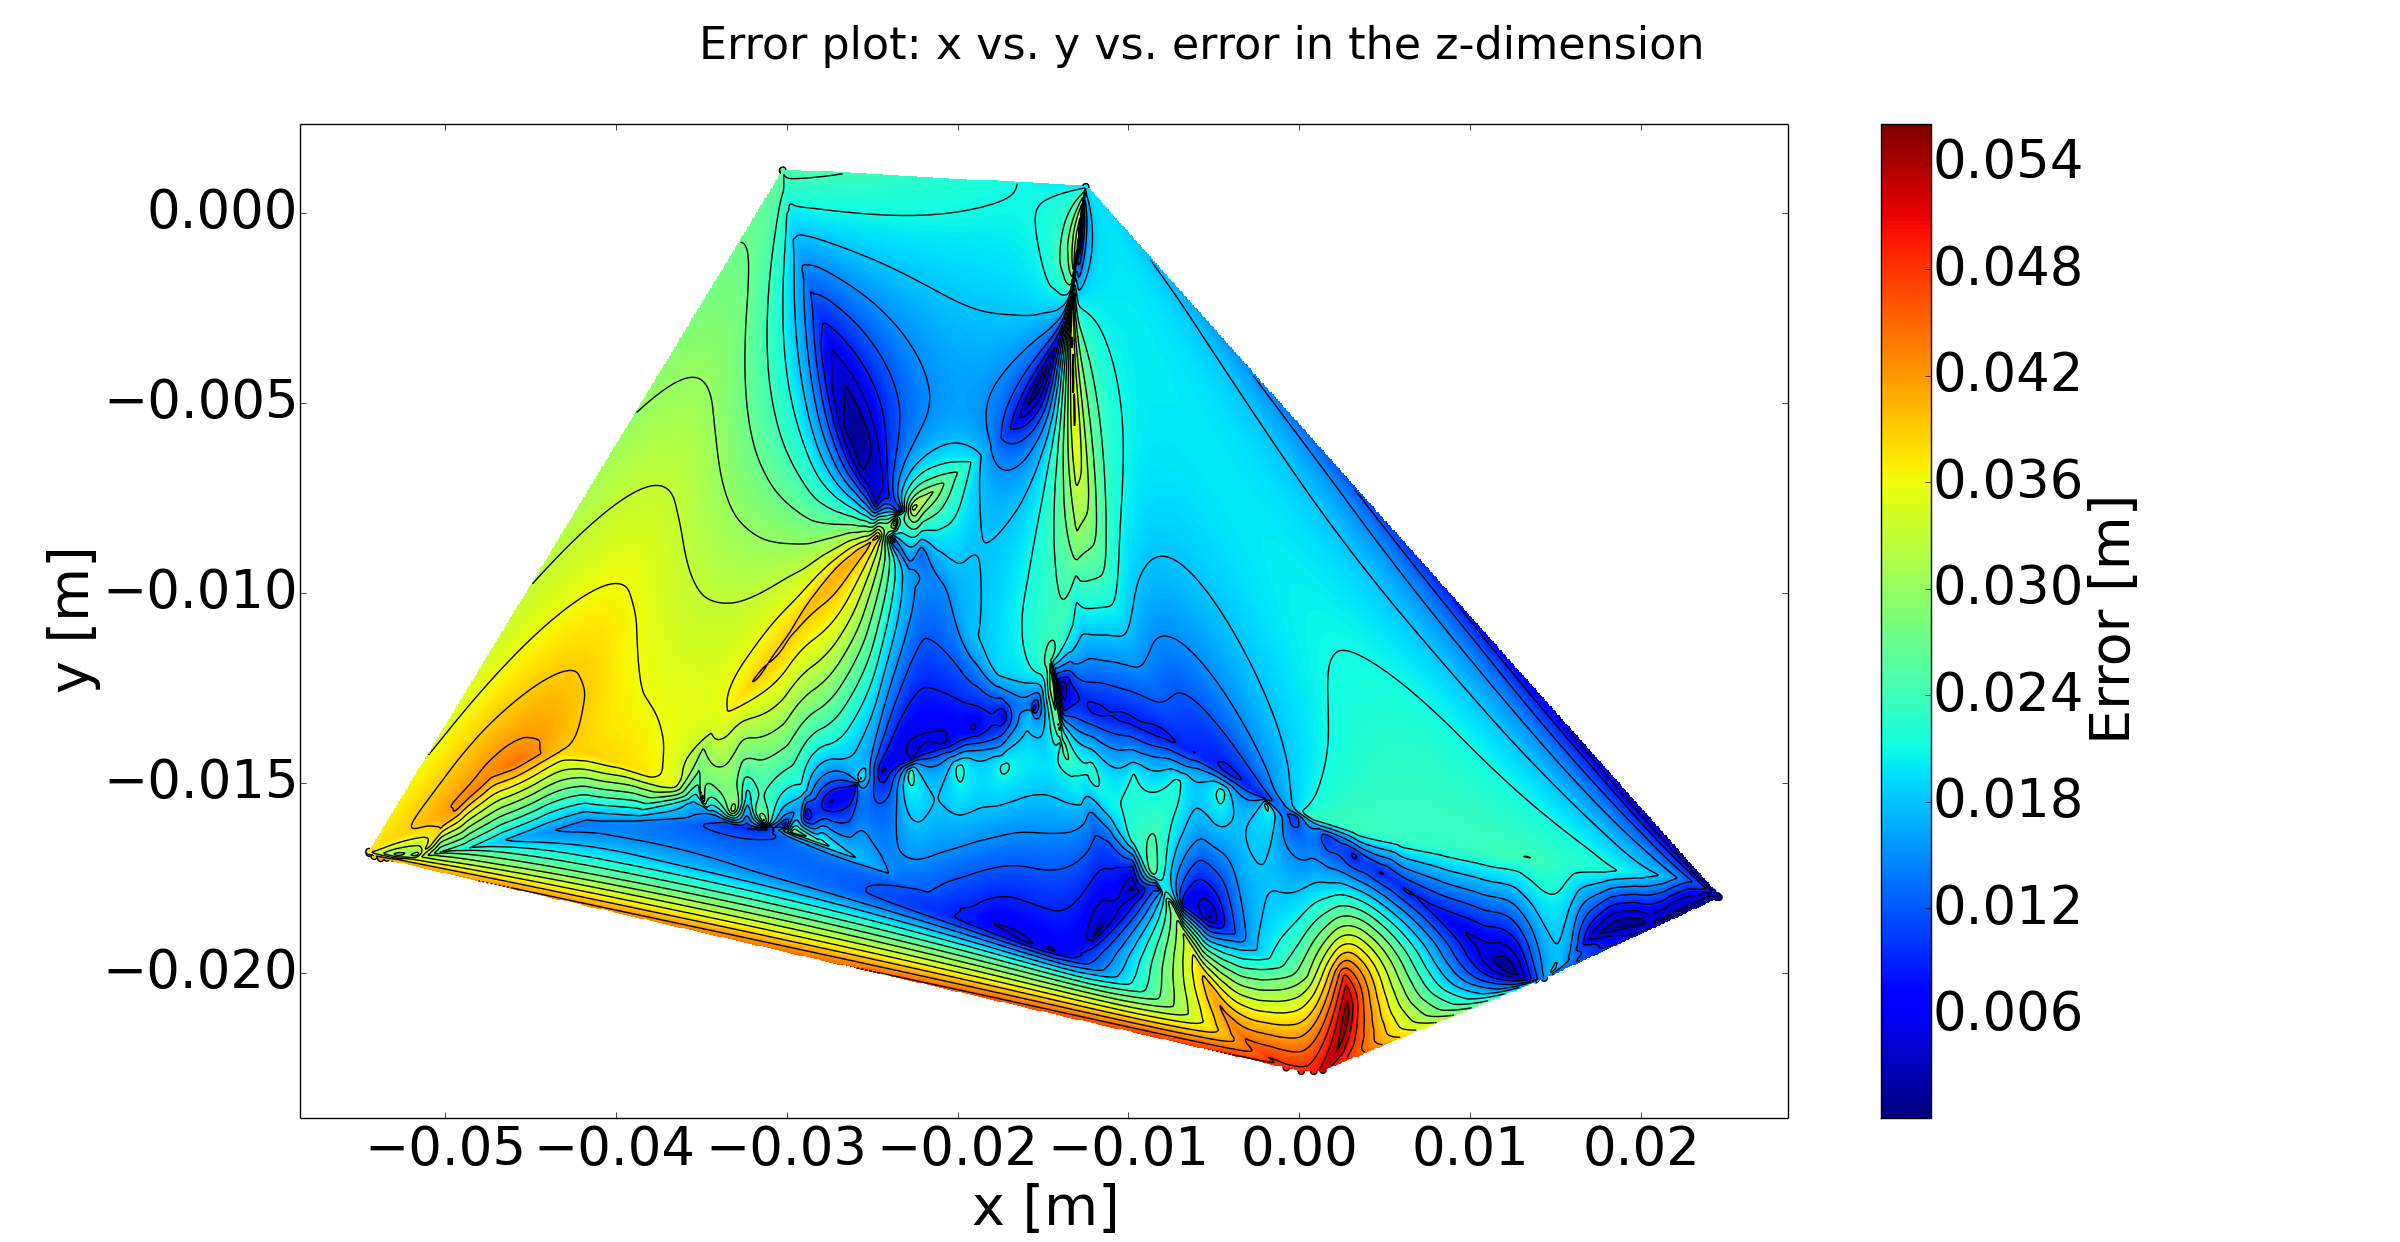
\includegraphics[clip, trim = 20 0 150 0, width=\textwidth]{figures/chapter3/contour_z}
    \end{subfigure}
    \caption{Error contour plots for the position dimensions. Units in m.}
  \end{subfigure}
  ~
  \begin{subfigure}{0.48\textwidth}
    \begin{subfigure}{\textwidth}
      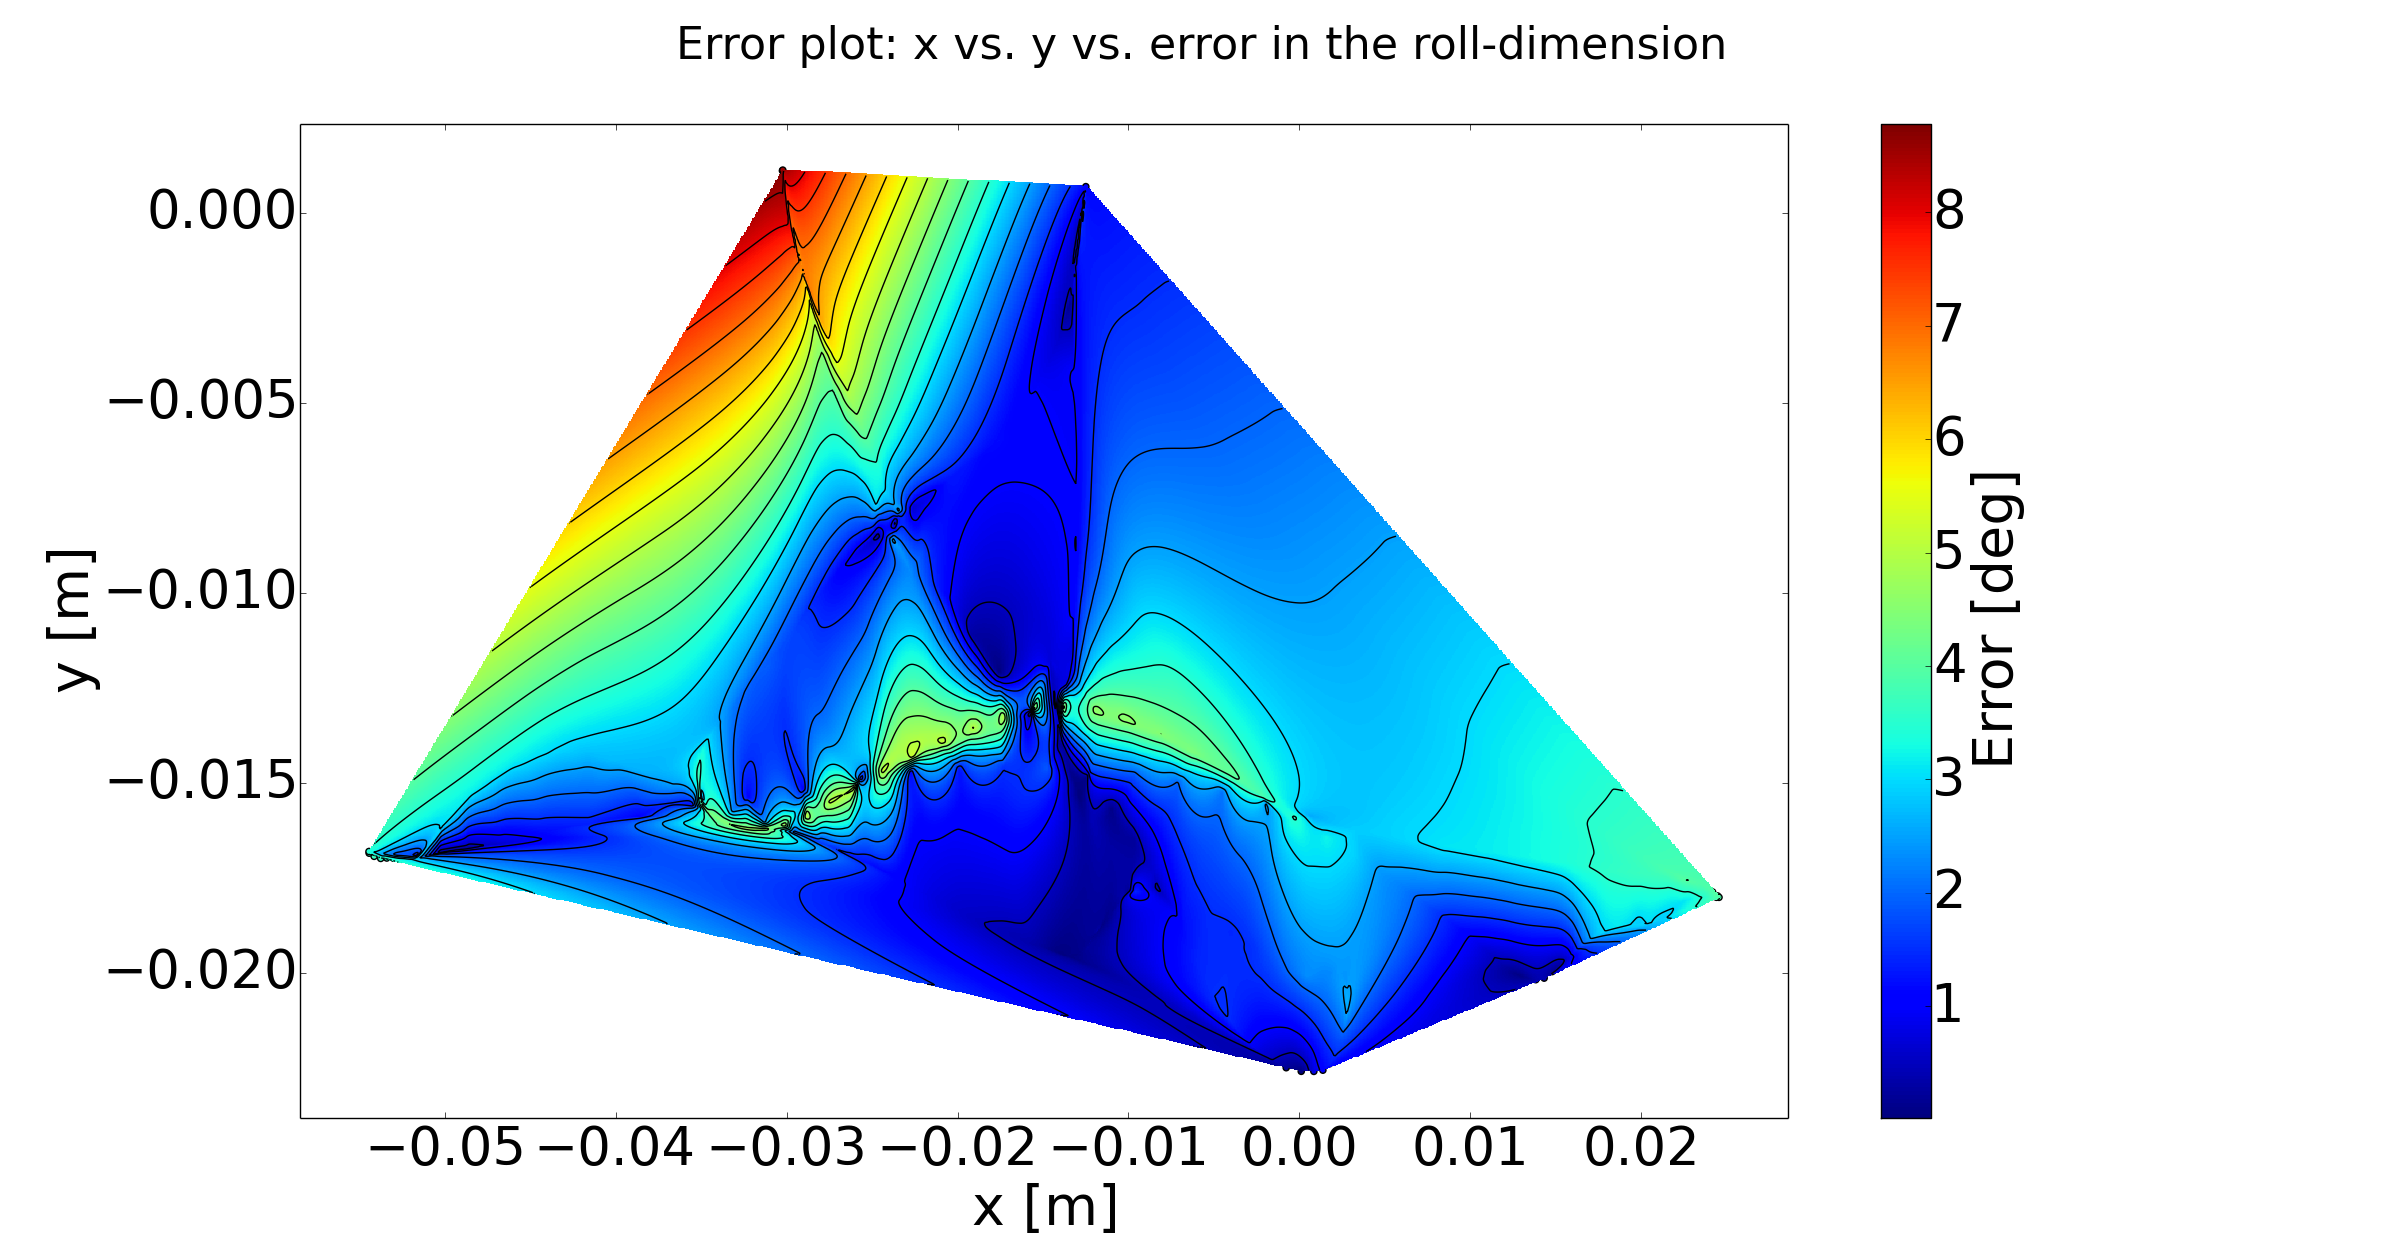
\includegraphics[clip, trim = 20 0 150 0, width=\textwidth]{figures/chapter3/contour_roll}
    \end{subfigure}
    \begin{subfigure}{\textwidth}
      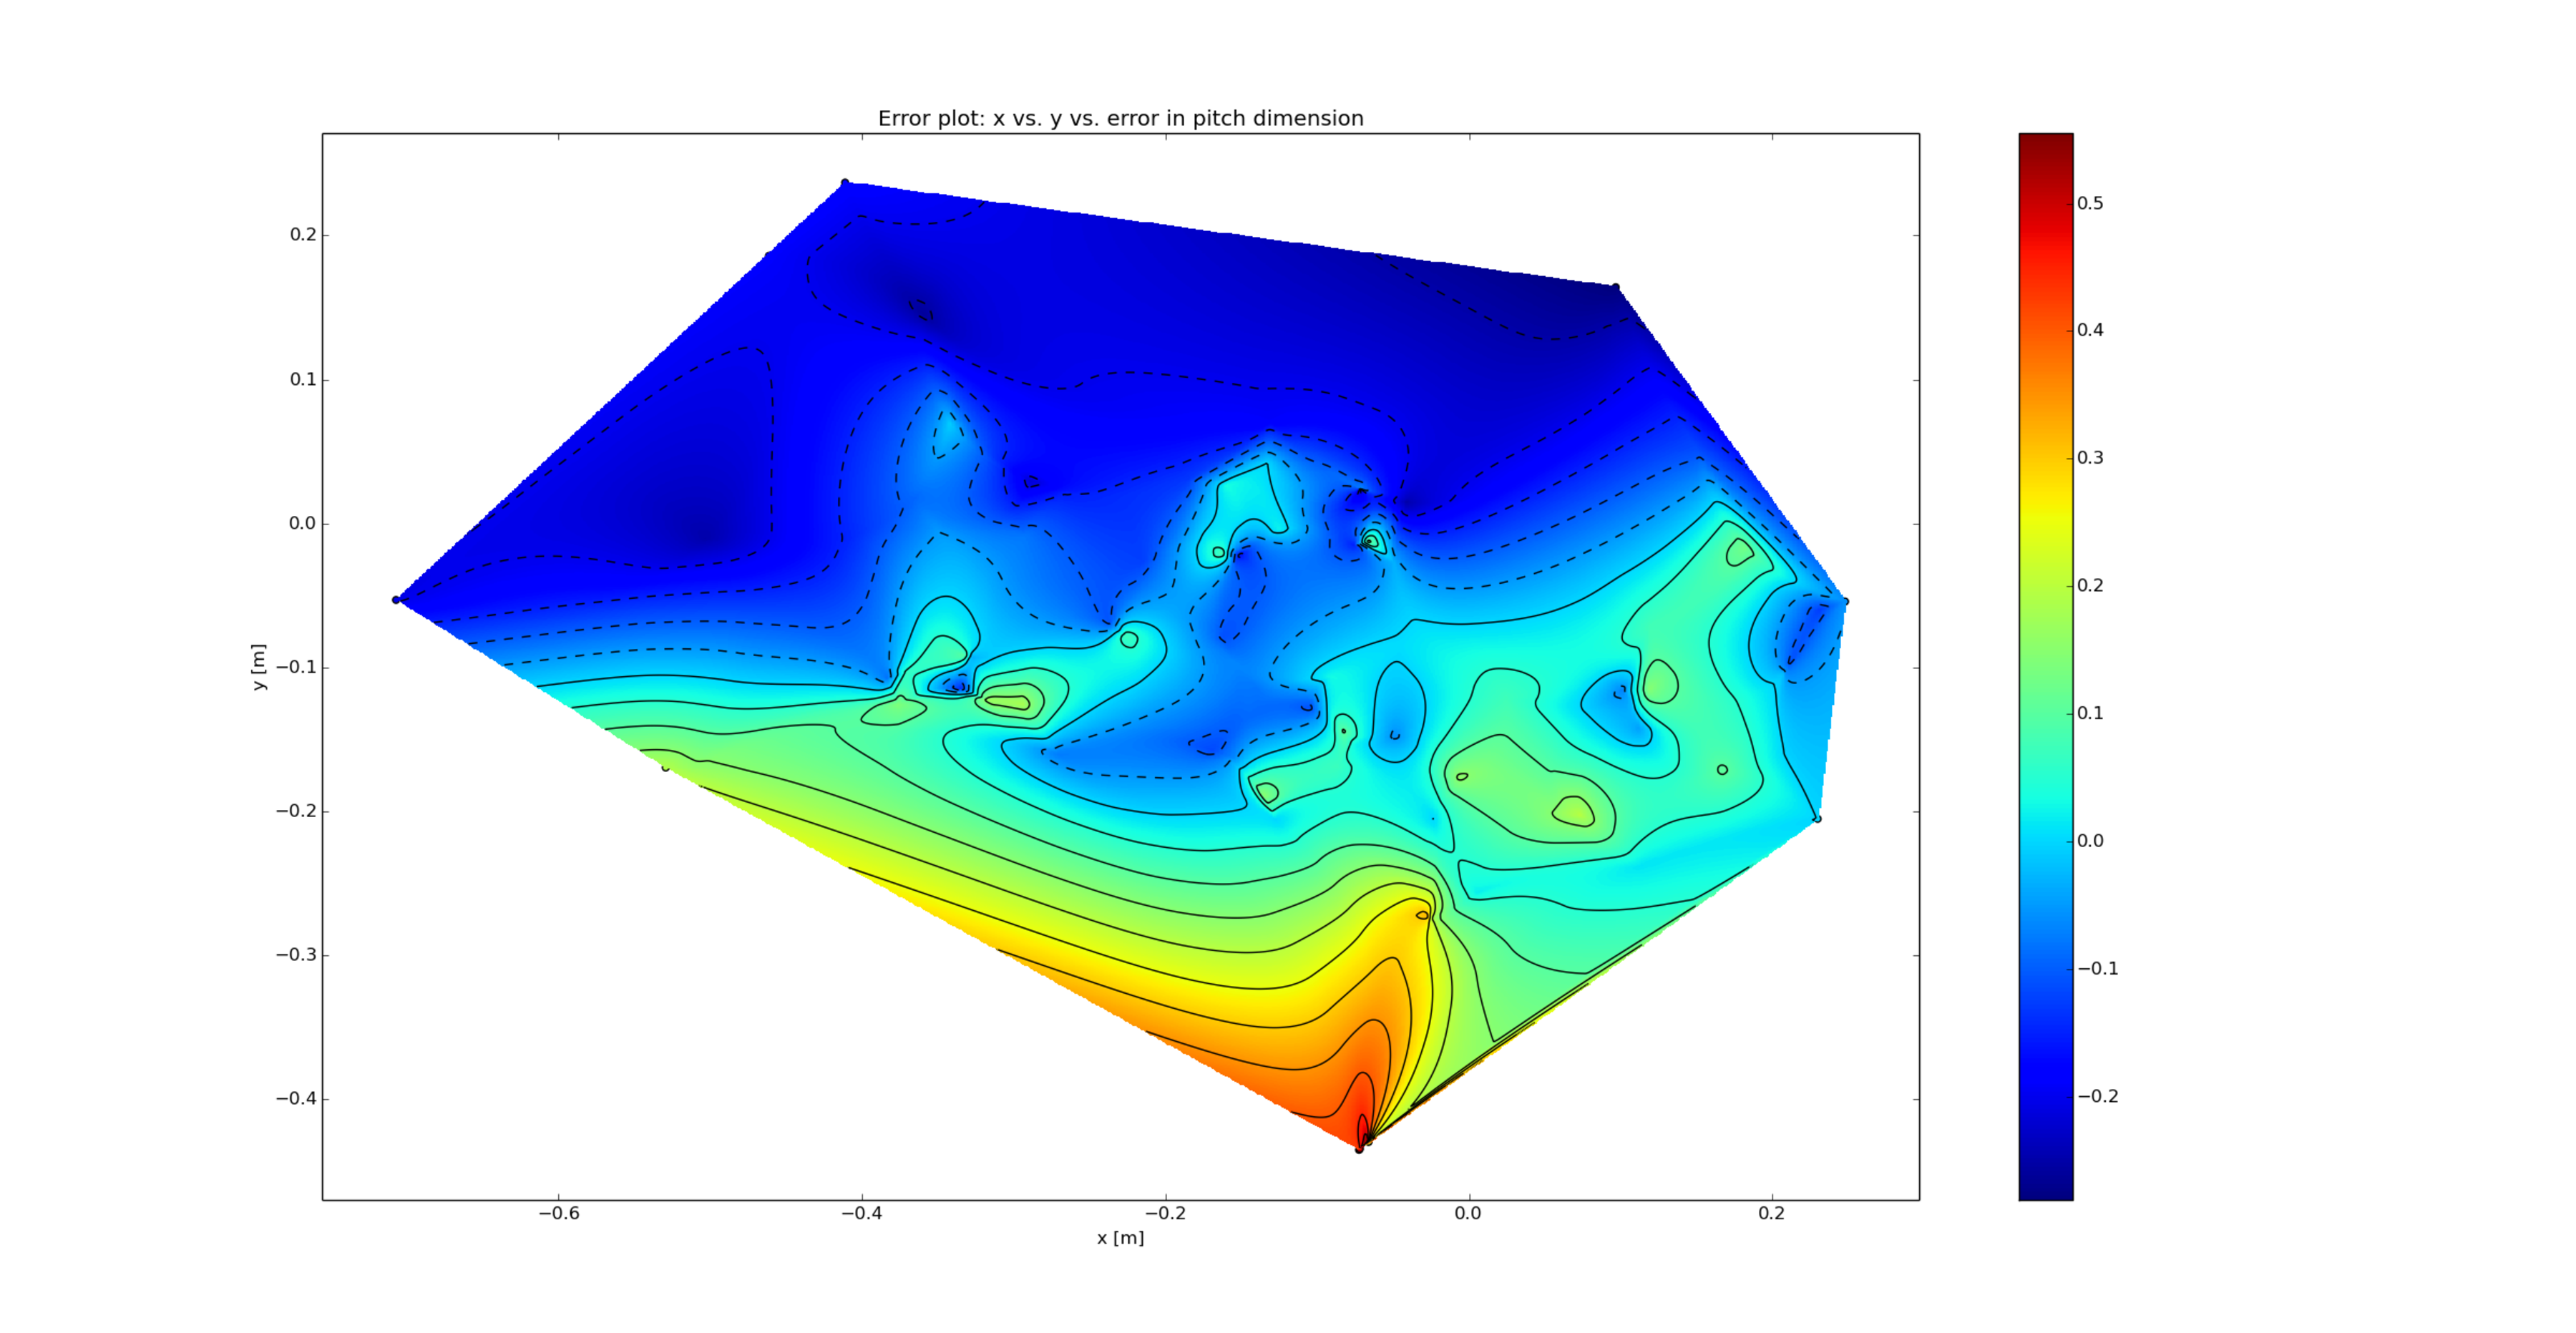
\includegraphics[clip, trim = 20 0 150 0, width=\textwidth]{figures/chapter3/contour_pitch}
    \end{subfigure}
    \begin{subfigure}{\textwidth}
      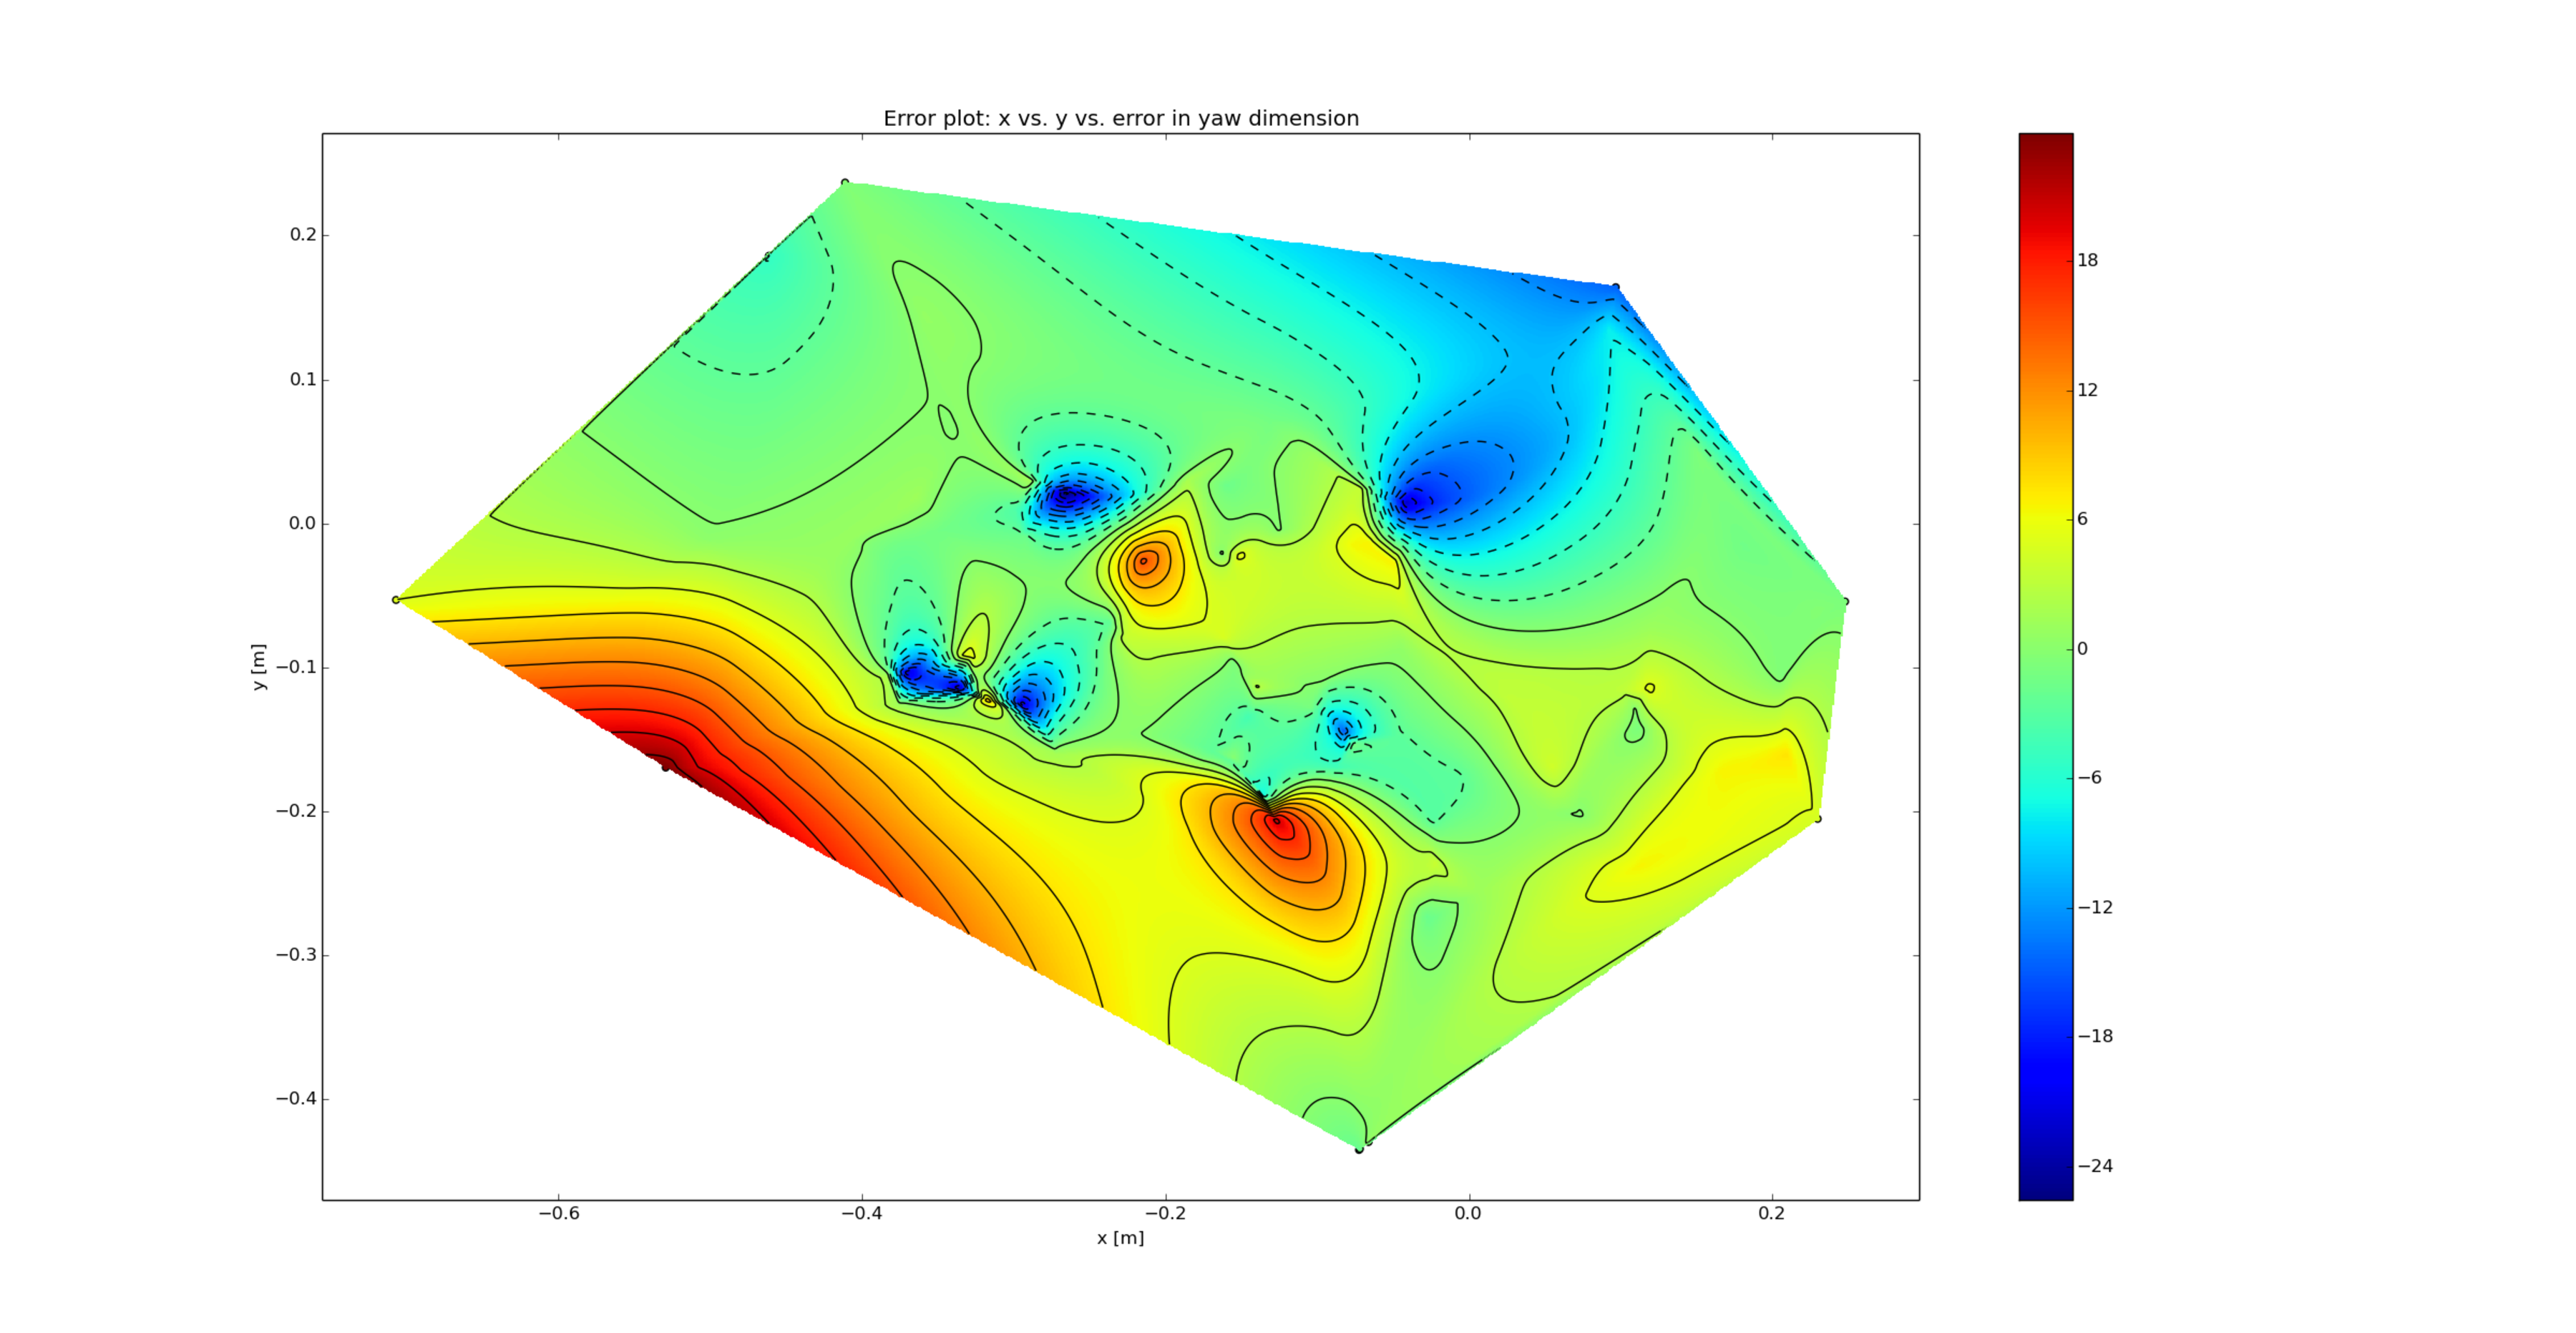
\includegraphics[clip, trim = 20 0 150 0, width=\textwidth]{figures/chapter3/contour_yaw}
    \end{subfigure}
    \caption{Error contour plots for the orientation dimensions. Units in \textdegree.}
  \end{subfigure}
  \caption[A collection of contour plots of the position and orientation vectors relative to one another]{A collection of contour plots of the position and orientation vectors relative to one another.}
  \label{fig:err-contour}
\end{figure*}

It can be seen from Figure~\ref{fig:err-contour} that the error in a dimension varies when the two other pose dimensions change. There are also multiple peaks, indicating that the error data is very complex. 

These plots, as well as the covariance matrix $\Sigma$, show that there is no clear indication on the CVS's accuracy, since it is a function of the pose of the calibration board relative to the CVS's camera. 

\section{Conclusion}

In this chapter, the design and layout of a computer vision measurement system (CVS) was discussed. The system consists of hardware and software components and the details of both were discussed. The system was tested in an indoor measurement facility to determine its measurement accuracy. With the ground-truth measurements produced by this indoor system, it was possible to optimise the intrinsic camera parameters and improve the accuracy of the CVS's pose measurement data.

The CVS's pose measurement error is not constant over all of the poses and it is therefore necessary to model this error as a function of the calibration board's pose relative to the CVS's camera. 
